% Options for packages loaded elsewhere
% Options for packages loaded elsewhere
\PassOptionsToPackage{unicode}{hyperref}
\PassOptionsToPackage{hyphens}{url}
\PassOptionsToPackage{dvipsnames,svgnames,x11names}{xcolor}
%
\documentclass[
  french,
  letterpaper,
]{report}
\usepackage{xcolor}
\usepackage{amsmath,amssymb}
\setcounter{secnumdepth}{5}
\usepackage{iftex}
\ifPDFTeX
  \usepackage[T1]{fontenc}
  \usepackage[utf8]{inputenc}
  \usepackage{textcomp} % provide euro and other symbols
\else % if luatex or xetex
  \usepackage{unicode-math} % this also loads fontspec
  \defaultfontfeatures{Scale=MatchLowercase}
  \defaultfontfeatures[\rmfamily]{Ligatures=TeX,Scale=1}
\fi
\usepackage{lmodern}
\ifPDFTeX\else
  % xetex/luatex font selection
\fi
% Use upquote if available, for straight quotes in verbatim environments
\IfFileExists{upquote.sty}{\usepackage{upquote}}{}
\IfFileExists{microtype.sty}{% use microtype if available
  \usepackage[]{microtype}
  \UseMicrotypeSet[protrusion]{basicmath} % disable protrusion for tt fonts
}{}
\makeatletter
\@ifundefined{KOMAClassName}{% if non-KOMA class
  \IfFileExists{parskip.sty}{%
    \usepackage{parskip}
  }{% else
    \setlength{\parindent}{0pt}
    \setlength{\parskip}{6pt plus 2pt minus 1pt}}
}{% if KOMA class
  \KOMAoptions{parskip=half}}
\makeatother
% Make \paragraph and \subparagraph free-standing
\makeatletter
\ifx\paragraph\undefined\else
  \let\oldparagraph\paragraph
  \renewcommand{\paragraph}{
    \@ifstar
      \xxxParagraphStar
      \xxxParagraphNoStar
  }
  \newcommand{\xxxParagraphStar}[1]{\oldparagraph*{#1}\mbox{}}
  \newcommand{\xxxParagraphNoStar}[1]{\oldparagraph{#1}\mbox{}}
\fi
\ifx\subparagraph\undefined\else
  \let\oldsubparagraph\subparagraph
  \renewcommand{\subparagraph}{
    \@ifstar
      \xxxSubParagraphStar
      \xxxSubParagraphNoStar
  }
  \newcommand{\xxxSubParagraphStar}[1]{\oldsubparagraph*{#1}\mbox{}}
  \newcommand{\xxxSubParagraphNoStar}[1]{\oldsubparagraph{#1}\mbox{}}
\fi
\makeatother


\usepackage{longtable,booktabs,array}
\usepackage{calc} % for calculating minipage widths
% Correct order of tables after \paragraph or \subparagraph
\usepackage{etoolbox}
\makeatletter
\patchcmd\longtable{\par}{\if@noskipsec\mbox{}\fi\par}{}{}
\makeatother
% Allow footnotes in longtable head/foot
\IfFileExists{footnotehyper.sty}{\usepackage{footnotehyper}}{\usepackage{footnote}}
\makesavenoteenv{longtable}
\usepackage{graphicx}
\makeatletter
\newsavebox\pandoc@box
\newcommand*\pandocbounded[1]{% scales image to fit in text height/width
  \sbox\pandoc@box{#1}%
  \Gscale@div\@tempa{\textheight}{\dimexpr\ht\pandoc@box+\dp\pandoc@box\relax}%
  \Gscale@div\@tempb{\linewidth}{\wd\pandoc@box}%
  \ifdim\@tempb\p@<\@tempa\p@\let\@tempa\@tempb\fi% select the smaller of both
  \ifdim\@tempa\p@<\p@\scalebox{\@tempa}{\usebox\pandoc@box}%
  \else\usebox{\pandoc@box}%
  \fi%
}
% Set default figure placement to htbp
\def\fps@figure{htbp}
\makeatother


% definitions for citeproc citations
\NewDocumentCommand\citeproctext{}{}
\NewDocumentCommand\citeproc{mm}{%
  \begingroup\def\citeproctext{#2}\cite{#1}\endgroup}
\makeatletter
 % allow citations to break across lines
 \let\@cite@ofmt\@firstofone
 % avoid brackets around text for \cite:
 \def\@biblabel#1{}
 \def\@cite#1#2{{#1\if@tempswa , #2\fi}}
\makeatother
\newlength{\cslhangindent}
\setlength{\cslhangindent}{1.5em}
\newlength{\csllabelwidth}
\setlength{\csllabelwidth}{3em}
\newenvironment{CSLReferences}[2] % #1 hanging-indent, #2 entry-spacing
 {\begin{list}{}{%
  \setlength{\itemindent}{0pt}
  \setlength{\leftmargin}{0pt}
  \setlength{\parsep}{0pt}
  % turn on hanging indent if param 1 is 1
  \ifodd #1
   \setlength{\leftmargin}{\cslhangindent}
   \setlength{\itemindent}{-1\cslhangindent}
  \fi
  % set entry spacing
  \setlength{\itemsep}{#2\baselineskip}}}
 {\end{list}}
\usepackage{calc}
\newcommand{\CSLBlock}[1]{\hfill\break\parbox[t]{\linewidth}{\strut\ignorespaces#1\strut}}
\newcommand{\CSLLeftMargin}[1]{\parbox[t]{\csllabelwidth}{\strut#1\strut}}
\newcommand{\CSLRightInline}[1]{\parbox[t]{\linewidth - \csllabelwidth}{\strut#1\strut}}
\newcommand{\CSLIndent}[1]{\hspace{\cslhangindent}#1}

\ifLuaTeX
\usepackage[bidi=basic]{babel}
\else
\usepackage[bidi=default]{babel}
\fi
% get rid of language-specific shorthands (see #6817):
\let\LanguageShortHands\languageshorthands
\def\languageshorthands#1{}


\setlength{\emergencystretch}{3em} % prevent overfull lines

\providecommand{\tightlist}{%
  \setlength{\itemsep}{0pt}\setlength{\parskip}{0pt}}



 


\usepackage{multirow}
\usepackage{longtable}
\makeatletter
\@ifpackageloaded{tcolorbox}{}{\usepackage[skins,breakable]{tcolorbox}}
\@ifpackageloaded{fontawesome5}{}{\usepackage{fontawesome5}}
\definecolor{quarto-callout-color}{HTML}{909090}
\definecolor{quarto-callout-note-color}{HTML}{0758E5}
\definecolor{quarto-callout-important-color}{HTML}{CC1914}
\definecolor{quarto-callout-warning-color}{HTML}{EB9113}
\definecolor{quarto-callout-tip-color}{HTML}{00A047}
\definecolor{quarto-callout-caution-color}{HTML}{FC5300}
\definecolor{quarto-callout-color-frame}{HTML}{acacac}
\definecolor{quarto-callout-note-color-frame}{HTML}{4582ec}
\definecolor{quarto-callout-important-color-frame}{HTML}{d9534f}
\definecolor{quarto-callout-warning-color-frame}{HTML}{f0ad4e}
\definecolor{quarto-callout-tip-color-frame}{HTML}{02b875}
\definecolor{quarto-callout-caution-color-frame}{HTML}{fd7e14}
\makeatother
\makeatletter
\@ifpackageloaded{bookmark}{}{\usepackage{bookmark}}
\makeatother
\makeatletter
\@ifpackageloaded{caption}{}{\usepackage{caption}}
\AtBeginDocument{%
\ifdefined\contentsname
  \renewcommand*\contentsname{Table des matières}
\else
  \newcommand\contentsname{Table des matières}
\fi
\ifdefined\listfigurename
  \renewcommand*\listfigurename{Liste des Figures}
\else
  \newcommand\listfigurename{Liste des Figures}
\fi
\ifdefined\listtablename
  \renewcommand*\listtablename{Liste des Tables}
\else
  \newcommand\listtablename{Liste des Tables}
\fi
\ifdefined\figurename
  \renewcommand*\figurename{Figure}
\else
  \newcommand\figurename{Figure}
\fi
\ifdefined\tablename
  \renewcommand*\tablename{Table}
\else
  \newcommand\tablename{Table}
\fi
}
\@ifpackageloaded{float}{}{\usepackage{float}}
\floatstyle{ruled}
\@ifundefined{c@chapter}{\newfloat{codelisting}{h}{lop}}{\newfloat{codelisting}{h}{lop}[chapter]}
\floatname{codelisting}{Listing}
\newcommand*\listoflistings{\listof{codelisting}{Liste des Listings}}
\makeatother
\makeatletter
\makeatother
\makeatletter
\@ifpackageloaded{caption}{}{\usepackage{caption}}
\@ifpackageloaded{subcaption}{}{\usepackage{subcaption}}
\makeatother
\usepackage{bookmark}
\IfFileExists{xurl.sty}{\usepackage{xurl}}{} % add URL line breaks if available
\urlstyle{same}
\hypersetup{
  pdftitle={Campagne 2025 des Observatoires ruraux d'Alaotra et Marovoay},
  pdfauthor={Veromanitra Ramizason, Bezaka Rivolala, Thierry Razanakoto, Holimalala Randriamanampisoa, Florent Bédécarrats},
  pdflang={fr},
  colorlinks=true,
  linkcolor={blue},
  filecolor={Maroon},
  citecolor={Blue},
  urlcolor={Blue},
  pdfcreator={LaTeX via pandoc}}


\title{Campagne 2025 des Observatoires ruraux d'Alaotra et Marovoay}
\usepackage{etoolbox}
\makeatletter
\providecommand{\subtitle}[1]{% add subtitle to \maketitle
  \apptocmd{\@title}{\par {\large #1 \par}}{}{}
}
\makeatother
\subtitle{Rapport consolidé d'enquêtes}
\author{Veromanitra Ramizason, Bezaka Rivolala, Thierry Razanakoto,
Holimalala Randriamanampisoa, Florent Bédécarrats}
\date{2026-03-15}
\begin{document}
\maketitle

\renewcommand*\contentsname{Table des matières}
{
\hypersetup{linkcolor=}
\setcounter{tocdepth}{2}
\tableofcontents
}

\bookmarksetup{startatroot}

\chapter*{Introduction}\label{introduction}
\addcontentsline{toc}{chapter}{Introduction}

\markboth{Introduction}{Introduction}

\begin{figure}[H]

{\centering \pandocbounded{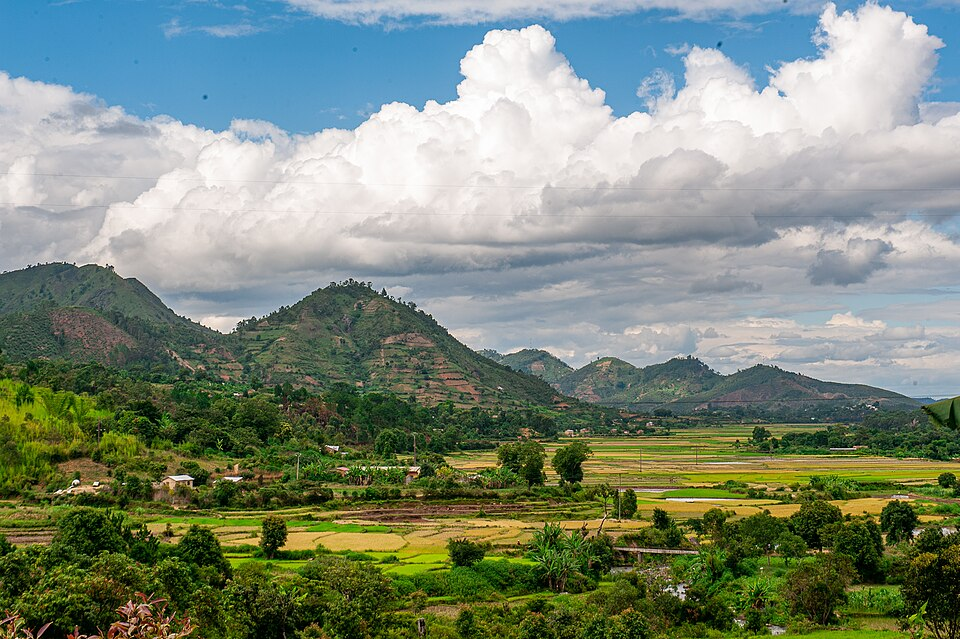
\includegraphics[keepaspectratio]{images/cover.jpg}}

}

\caption{Rizière dans la région d'Alaotra Mangoro. Photo : Leja Mitarika
/ NJProduction,
\href{https://creativecommons.org/licenses/by-sa/4.0/}{CC BY-SA 4.0},
via
\href{https://commons.wikimedia.org/wiki/File:Rizi\%C3\%A8re_d\%27alaotra_Mangoro.jpg}{Wikimedia
Commons}.}

\end{figure}%

Ce document présente le traitement et l'analyse des données des
observatoires ruraux d'Alaotra et de Marovoay pour la campagne 2025. La
période de référence s'étend d'octobre 2024 à septembre 2025. Ces
données ont été récoltées afin d'étudier l'évaluation d'impact de la
conservation sur les conditions de vie des ménages aux alentours des
aires protégées.

\begin{tcolorbox}[enhanced jigsaw, colframe=quarto-callout-note-color-frame, colback=white, titlerule=0mm, colbacktitle=quarto-callout-note-color!10!white, toptitle=1mm, opacitybacktitle=0.6, title=\textcolor{quarto-callout-note-color}{\faInfo}\hspace{0.5em}{Confidentialité statistique}, left=2mm, leftrule=.75mm, bottomtitle=1mm, coltitle=black, arc=.35mm, rightrule=.15mm, bottomrule=.15mm, toprule=.15mm, opacityback=0, breakable]

Par souci de confidentialité, les cellules de tableaux reposant sur un
effectif inférieur à 5 observations sont supprimées et remplacées par la
mention « \textless{} 5 ». Les fichiers téléchargeables par site
appliquent la même règle.

\end{tcolorbox}

Au préalable, une analyse exploratoire des données est essentielle avec
les étapes suivantes :

\begin{itemize}
\item
  le chargement des données ;
\item
  la vérification de la complétude des données ;
\item
  l'apurement des données ;
\item
  les analyses descriptives des données.
\end{itemize}

Brèves historiques des OR: 1995-2015

Description d'Alaotra

Description de Marovoay

Pour cette année 2025, deux observatoires ruraux ont fait l'objet
d'enquête auprès des ménages ruraux.

Hameaux pour Alaotra : Hameaux pour Marovoay : Madiromiongana, Bepako,
Maroala, Ampijoroa

Nombres de ménages enquêtés :

\bookmarksetup{startatroot}

\chapter{Description de l'enquête}\label{description-de-lenquuxeate}

\begin{tcolorbox}[enhanced jigsaw, colframe=quarto-callout-warning-color-frame, colback=white, titlerule=0mm, colbacktitle=quarto-callout-warning-color!10!white, toptitle=1mm, opacitybacktitle=0.6, title=\textcolor{quarto-callout-warning-color}{\faExclamationTriangle}\hspace{0.5em}{Travail de vérification en cours}, left=2mm, leftrule=.75mm, bottomtitle=1mm, coltitle=black, arc=.35mm, rightrule=.15mm, bottomrule=.15mm, toprule=.15mm, opacityback=0, breakable]

Les résultats présentés ci-dessous sont provisoires, et sont
susceptibles de faire l'objet de corrections.

\end{tcolorbox}

\section{Contexte et objectifs}\label{contexte-et-objectifs}

Les Observatoires Ruraux (OR) de Madagascar sont un dispositif d'enquête
longitudinale auprès de ménages ruraux, mis en place à partir de 1995
dans le cadre du réseau des observatoires ruraux coordonné par l'IRD et
l'INSTAT, puis le Ministère de l'agriculture. Deux OR font l'objet de
cette campagne d'enquête en 2025 :

\begin{itemize}
\tightlist
\item
  \textbf{Alaotra}, situé dans la région Alaotra-Mangoro, dans les
  districts d'Ambatondrazaka et d'Amparafaravola. L'Alaotra est le
  premier grenier à riz de Madagascar, caractérisé par de vastes plaines
  irriguées et des périmètres aménagés.
\item
  \textbf{Marovoay} , situé dans la région Boeny, dans le district de
  Marovoay. Marovoay constitue le deuxième pôle rizicole du pays, avec
  une production reposant sur l'irrigation par les eaux du fleuve
  Betsiboka.
\end{itemize}

\textbf{Marovoay.} L'observatoire de Marovoay est situé dans la plaine
alluviale du fleuve Betsiboka, au nord-ouest de Madagascar. La zone
d'enquête s'organise autour de quatre fokontany --- Ampijoroa et Maroala
sur la rive gauche, Bepako et Madiromiongana sur la rive droite ---
séparés par le fleuve. La proximité du Parc national d'Ankarafantsika,
dont les limites ont été étendues en 2002, confère à cette zone un
intérêt particulier pour l'étude des interactions entre conservation et
développement rural. L'économie locale repose principalement sur la
riziculture irriguée, complétée par l'élevage bovin et les cultures de
rente.

\textbf{Alaotra.} L'observatoire de l'Alaotra se situe dans la cuvette
du lac Alaotra, le plus grand lac de Madagascar, au centre-est de l'île.
La zone d'enquête couvre sept fokontany répartis dans les districts
d'Ambatondrazaka et d'Amparafaravola : Avaradrano, Feramanga Atsimo et
Mangabe au sud du lac, Analamiranga, Maritampona, Ambohidrony et
Ambatomanga à l'ouest. Le lac Alaotra est une nouvelle aire protégée
établie temporairement en 2007, puis définitivement en 2015. Il est
entouré de marais et de zones humides qui abritent des espèces
endémiques. Premier bassin rizicole du pays, la région est aussi
caractérisée par une pression foncière croissante et une dynamique de
déforestation des bassins versants.

Ces deux observatoires ont été enquêtés de manière régulière entre 1995
et 2014 (Marovoay) et 1999 et 2014 (Alaotra), avec une seule
interruption l'année 2009 en raison de la crise politique qui a secoué
le pays. La campagne 2025, réalisée par le projet BETSAKA, renoue avec
ce suivi après une interruption de plus de dix ans. L'enquête conserve
les instruments et la méthodologie des campagnes antérieures, tout en
reprenant des ajustements faits dans le cadre de l'observatoire du Makay
en 2022 et 2024, et en les adaptant au contexte actuel.

\begin{quote}
Introduire ici un paragraphe qui liste les modifications introduites
pour cette campagne : allègement du questionnaire, modules développés
pour le Makay qui ont été repris, nouveau formulaire de consentement
éclairé\ldots{}
\end{quote}

La période de référence couvre les douze mois précédant l'interview,
soit du 1\textsuperscript{er} octobre 2024 au 30 septembre 2025.

\emph{Note méthodologique.} Après plus de dix ans d'interruption (la
dernière campagne régulière date de 2014), la reconstitution du panel de
ménages constitue un défi majeur. Le suivi longitudinal est affecté par
l'attrition (décès, migration, éclatement des ménages), ce qui a conduit
à compléter le panel historique par un nouveau tirage aléatoire. Les
comparaisons inter-temporelles doivent donc être interprétées avec
prudence, en tenant compte de ce renouvellement partiel de
l'échantillon. Un chapitre d'approfondissement est consacré à cette
question, voir Chapitre~\ref{sec-representativite}.

\section{Méthodologie}\label{muxe9thodologie}

L'enquête reprend le protocole des campagnes antérieures des
Observatoires Ruraux. Le questionnaire ménage couvre l'ensemble des
dimensions socio-économiques : démographie, habitat, activités agricoles
et non agricoles, foncier, revenus, sécurité alimentaire, environnement
et événements climatiques.

Les unités d'observation sont les ménages résidant dans les hameaux
échantillonnés. L'échantillon de 2025 vise à reconstituer autant que
possible le panel de ménages suivis lors des campagnes précédentes,
complété par de nouveaux ménages en remplacement de ceux ayant quitté la
zone ou disparus.

Les enquêteurs ont été formés par les superviseurs avant le déploiement
sur le terrain. La saisie des données a été réalisée à l'aide de masques
de saisie dédiés.

\begin{tcolorbox}[enhanced jigsaw, colframe=quarto-callout-note-color-frame, colback=white, titlerule=0mm, colbacktitle=quarto-callout-note-color!10!white, toptitle=1mm, opacitybacktitle=0.6, title=\textcolor{quarto-callout-note-color}{\faInfo}\hspace{0.5em}{Note}, left=2mm, leftrule=.75mm, bottomtitle=1mm, coltitle=black, arc=.35mm, rightrule=.15mm, bottomrule=.15mm, toprule=.15mm, opacityback=0, breakable]

Le protocole éthique de l'enquête a fait l'objet d'une approbation. Il
est présenté en annexe du rapport.

\end{tcolorbox}

\section{Localisation des sites
enquêtés}\label{localisation-des-sites-enquuxeatuxe9s}

Les coordonnées GPS des hameaux enquêtés ont été relevées lors de la
campagne. La carte ci-dessous présente la localisation approximative de
chaque fokontany, calculée comme le centroïde des hameaux qui le
composent. Les deux observatoires se situent dans le nord-ouest
(Marovoay) et le centre-est (Alaotra) de Madagascar.

\begin{figure}[H]

{\centering \pandocbounded{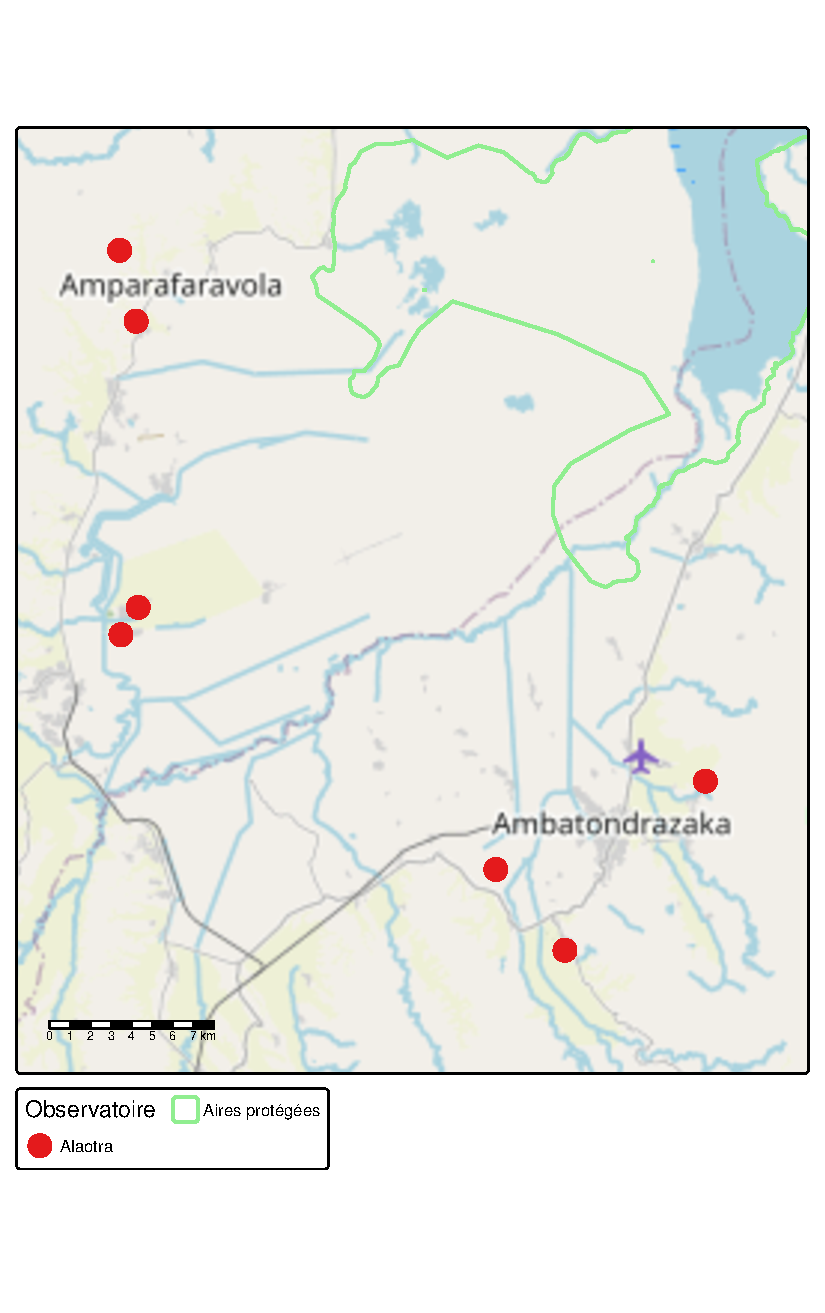
\includegraphics[keepaspectratio]{01_description_files/figure-pdf/carte_sites-1.pdf}}

}

\caption{Localisation approximative des fokontany enquêtés (centroïde
des hameaux)}

\end{figure}%

\section{Ménages enquêtés}\label{muxe9nages-enquuxeatuxe9s}

Au total, 1026 ménages ont été enquêtés : 519 à Marovoay et 507 à
Alaotra. Voir Table~\ref{tbl-men-obs}.

\begin{table}

\caption{\label{tbl-men-obs}Répartition des ménages et des individus
selon les observatoires}

\centering{

\fontsize{12.0pt}{14.0pt}\selectfont
\begin{tabular*}{\linewidth}{@{\extracolsep{\fill}}lrrrr}
\toprule
Observatoire & Ménages & Individus & \% ménages & \% individus \\ 
\midrule\addlinespace[2.5pt]
Marovoay & 519 & 2 297 & 50.6 & 53.8 \\ 
Alaotra & 507 & 1 975 & 49.4 & 46.2 \\ 
{\bfseries {Ensemble}} & {\bfseries {1 026}} & {\bfseries {4 272}} & {\bfseries {100.0}} & {\bfseries {100.0}} \\ 
\bottomrule
\end{tabular*}
\begin{minipage}{\linewidth}
\textbf{Source : Enquête auprès des OR 2025}\\
\end{minipage}

}

\end{table}%

\subsection{Dénombrement et taux de
sondage}\label{duxe9nombrement-et-taux-de-sondage}

Le dénombrement préalable à l'enquête a recensé l'ensemble des ménages
résidant dans les hameaux échantillonnés. Le
Table~\ref{tbl-denombrement} confronte le nombre de ménages dénombrés au
nombre de ménages effectivement enquêtés. Le taux de sondage global est
de l'ordre de 18 \%.

\begin{table}

\caption{\label{tbl-denombrement}Dénombrement et taux de sondage par
observatoire}

\centering{

\fontsize{12.0pt}{14.0pt}\selectfont
\begin{tabular*}{\linewidth}{@{\extracolsep{\fill}}lrrrr}
\toprule
Observatoire & Toits dénombrés & Ménages dénombrés & Ménages enquêtés & Taux de sondage (\%) \\ 
\midrule\addlinespace[2.5pt]
Alaotra & 6 142 & 6 210 & 507 & 8.2 \\ 
Marovoay & 2 370 & 2 506 & 519 & 20.7 \\ 
\bottomrule
\end{tabular*}
\begin{minipage}{\linewidth}
\textbf{Source : Synthèse Dénombrement OR 2025 \& Enquête auprès des OR 2025}\\
\end{minipage}

}

\end{table}%

\subsection{Répartition par hameau}\label{ruxe9partition-par-hameau}

Le Table~\ref{tbl-men-hameau} détaille le nombre de ménages enquêtés
dans chacun des hameaux, regroupés par site au sein de chaque
observatoire.

\begin{table}

\caption{\label{tbl-men-hameau}Répartition des ménages enquêtés par
hameau}

\centering{

\fontsize{12.0pt}{14.0pt}\selectfont
\begin{tabular*}{\linewidth}{@{\extracolsep{\fill}}lrr}
\toprule
Hameau & Ménages & \% obs. \\ 
\midrule\addlinespace[2.5pt]
\multicolumn{3}{l}{{\bfseries {Alaotra}}} \\[2.5pt] 
\midrule\addlinespace[2.5pt]
Avaradrano & 90 & 17.8 \\ 
Feramanga Atsimo & 89 & 17.6 \\ 
Mangabe & 73 & 14.4 \\ 
Ambatomanga & 68 & 13.4 \\ 
Ambodivoara & 58 & 11.4 \\ 
Ambohidrony & 52 & 10.3 \\ 
Analamiranga & 46 & 9.1 \\ 
Ambatoharanana & 31 & 6.1 \\ 
{\bfseries {Ensemble}} & {\bfseries {507}} & {\bfseries {100.0}} \\ 
\midrule\addlinespace[2.5pt]
\multicolumn{3}{l}{{\bfseries {Marovoay}}} \\[2.5pt] 
\midrule\addlinespace[2.5pt]
Ampijoroa & 143 & 27.6 \\ 
Madiromiongana & 137 & 26.4 \\ 
Bepako & 123 & 23.7 \\ 
Maroala & 116 & 22.4 \\ 
{\bfseries {Ensemble}} & {\bfseries {519}} & {\bfseries {100.0}} \\ 
\bottomrule
\end{tabular*}
\begin{minipage}{\linewidth}
\textbf{Source : Enquête auprès des OR 2025}\\
\end{minipage}

}

\end{table}%

\section{Déroulement de l'enquête}\label{duxe9roulement-de-lenquuxeate}

\subsection{Période de collecte}\label{puxe9riode-de-collecte}

Les entretiens se sont déroulés entre début octobre et mi-novembre 2025.
Un entretien isolé a été réalisé à Marovoay le 3 septembre ; il est
exclu du chronogramme ci-dessous qui ne retient que les dates à partir
du 1\textsuperscript{er} octobre 2025. Le Figure~\ref{fig-chronogramme}
présente l'évolution cumulée du nombre d'entretiens réalisés.

\begin{figure}

\centering{

\pandocbounded{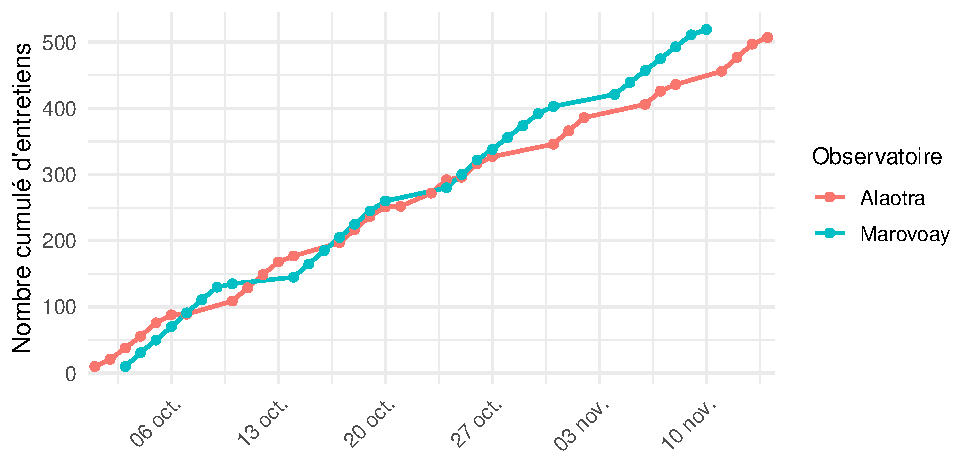
\includegraphics[keepaspectratio]{01_description_files/figure-pdf/fig-chronogramme-1.pdf}}

}

\caption{\label{fig-chronogramme}Fréquences cumulées des entretiens par
observatoire (à partir du 1er octobre 2025)}

\end{figure}%

\begin{table}

\caption{\label{tbl-periode}Période de collecte par observatoire}

\centering{

\fontsize{12.0pt}{14.0pt}\selectfont
\begin{tabular*}{\linewidth}{@{\extracolsep{\fill}}lrrrr}
\toprule
Observatoire & Début & {\bfseries {Fin}} & Jours d'enquête & Ménages \\ 
\midrule\addlinespace[2.5pt]
Alaotra & 1 October 2025 & 14 November 2025 & 32 & 507 \\ 
Marovoay & 3 October 2025 & 10 November 2025 & 30 & 518 \\ 
\bottomrule
\end{tabular*}
\begin{minipage}{\linewidth}
\textbf{Source : Enquête auprès des OR 2025}\\
\end{minipage}

}

\end{table}%

\subsection{Équipe d'enquête}\label{uxe9quipe-denquuxeate}

L'enquête a mobilisé 20 enquêteurs (10 par observatoire), encadrés par 6
superviseurs (3 par observatoire). La saisie des questionnaires a été
assurée par 4 opérateurs. Le Figure~\ref{fig-enqueteurs} présente le
nombre de questionnaires réalisés par chaque enquêteur (identifié par un
code anonyme).

\begin{figure}

\centering{

\pandocbounded{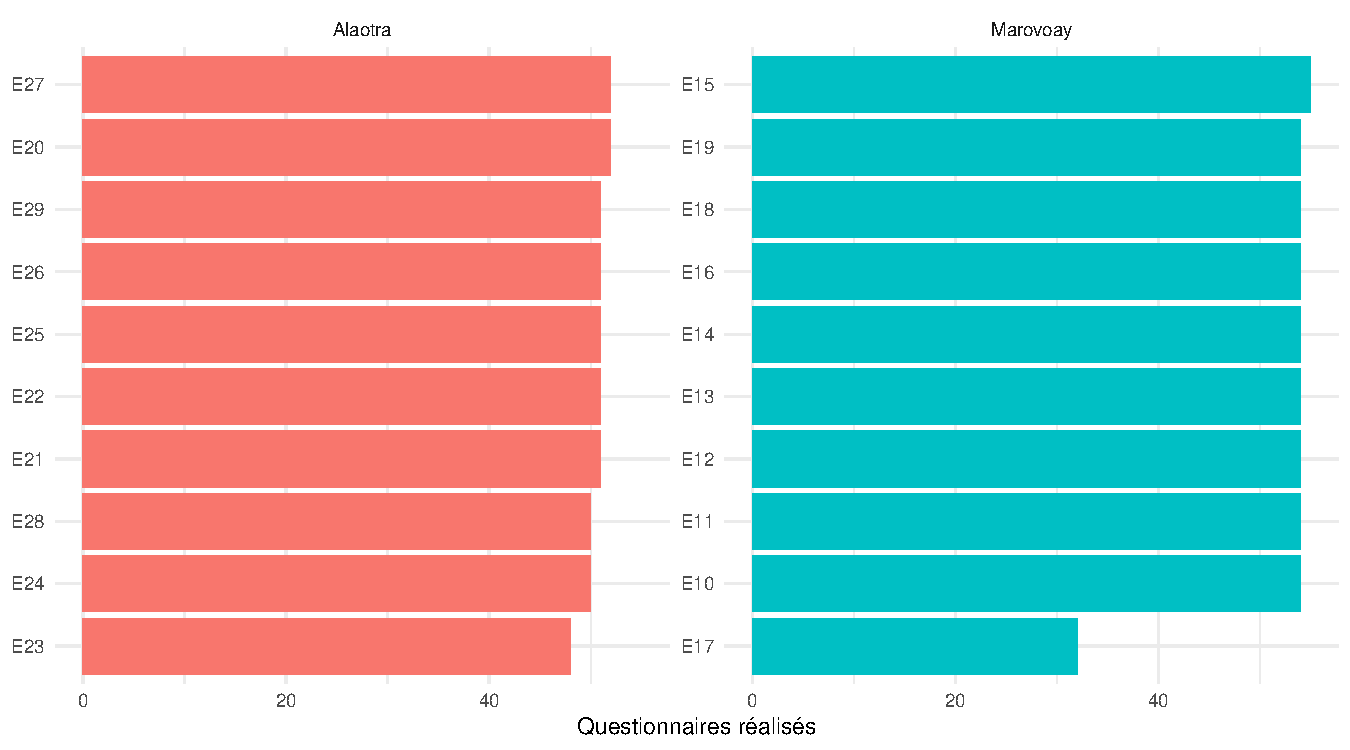
\includegraphics[keepaspectratio]{01_description_files/figure-pdf/fig-enqueteurs-1.pdf}}

}

\caption{\label{fig-enqueteurs}Nombre de questionnaires par enquêteur et
observatoire}

\end{figure}%

\begin{table}

\caption{\label{tbl-superviseurs}Nombre de questionnaires supervisés par
superviseur}

\centering{

\fontsize{12.0pt}{14.0pt}\selectfont
\begin{tabular*}{\linewidth}{@{\extracolsep{\fill}}lrr}
\toprule
{\bfseries {Superviseur}} & {\bfseries {Alaotra}} & {\bfseries {Marovoay}} \\ 
\midrule\addlinespace[2.5pt]
S01 & 172 & 86 \\ 
S02 & 166 & 217 \\ 
S03 & 169 & 216 \\ 
\bottomrule
\end{tabular*}
\begin{minipage}{\linewidth}
\textbf{Source : Enquête auprès des OR 2025}\\
\end{minipage}

}

\end{table}%

\begin{table}

\caption{\label{tbl-saisie}Nombre de questionnaires saisis par opérateur
de saisie}

\centering{

\fontsize{12.0pt}{14.0pt}\selectfont
\begin{tabular*}{\linewidth}{@{\extracolsep{\fill}}lr}
\toprule
Opérateur & {\bfseries {Questionnaires}} \\ 
\midrule\addlinespace[2.5pt]
OP01 & 252 \\ 
OP02 & 255 \\ 
OP03 & 260 \\ 
OP04 & 259 \\ 
\bottomrule
\end{tabular*}
\begin{minipage}{\linewidth}
\textbf{Source : Enquête auprès des OR 2025}\\
\end{minipage}

}

\end{table}%

\bookmarksetup{startatroot}

\chapter{Caractéristiques socio-démographiques des
ménages}\label{caractuxe9ristiques-socio-duxe9mographiques-des-muxe9nages}

Le ménage est l'unité de base de l'enquête. Cette section décrit la
composition des ménages, les caractéristiques des chefs de ménage et de
leurs membres, ainsi que l'évolution de ces indicateurs.

\begin{tcolorbox}[enhanced jigsaw, colframe=quarto-callout-warning-color-frame, colback=white, titlerule=0mm, colbacktitle=quarto-callout-warning-color!10!white, toptitle=1mm, opacitybacktitle=0.6, title=\textcolor{quarto-callout-warning-color}{\faExclamationTriangle}\hspace{0.5em}{Travail de vérification en cours}, left=2mm, leftrule=.75mm, bottomtitle=1mm, coltitle=black, arc=.35mm, rightrule=.15mm, bottomrule=.15mm, toprule=.15mm, opacityback=0, breakable]

Les résultats présentés ci-dessous sont provisoires, et sont
susceptibles de faire l'objet de corrections.

\end{tcolorbox}

\textbf{Marovoay.} À Marovoay, la structure des ménages est marquée par
l'hétérogénéité des stratégies économiques et des structures familiales.
La proximité de la ville de Marovoay et de la route nationale RN4
reliant Antananarivo à Mahajanga facilite les échanges et influence les
activités non agricoles des ménages.

\textbf{Alaotra.} Dans l'Alaotra, la riziculture irriguée constitue le
socle de l'économie domestique, et la taille des exploitations rizicoles
influence directement la structure et les revenus des ménages. Les
fokontany proches des périmètres irrigués (Avaradrano, Feramanga Atsimo)
présentent des profils économiques distincts de ceux situés en
périphérie de la cuvette (Analamiranga, Maritampona), où la dépendance
au riz pluvial et à l'élevage est plus marquée.

\emph{Note technique.} Les indicateurs démographiques présentés dans
cette section sont calculés à partir du fichier ménage
(\texttt{res\_deb}) et du fichier des membres (\texttt{res\_m\_a}). La
classification des activités principales s'appuie sur une nomenclature
sectorielle inspirée de la CITI Rév. 4. Les effectifs inférieurs à cinq
sont masqués par souci de confidentialité statistique. Les comparaisons
entre les deux observatoires doivent tenir compte de la différence de
taille des échantillons et de la structure spatiale des zones enquêtées.

\section{Description des ménages}\label{description-des-muxe9nages}

L'enquête a permis de recenser 4272 individus répartis dans 1026 ménages
au sein des deux observatoires.

\textbf{Alaotra.} La taille moyenne des ménages s'établit à 3.9
personnes.

\textbf{Marovoay.} La taille moyenne des ménages s'établit à 4.4
personnes.

\subsection{Taille des ménages par
observatoire}\label{taille-des-muxe9nages-par-observatoire}

\begin{table}

\caption{\label{tbl-men-obs}Taille moyenne des ménages par observatoire}

\centering{

\fontsize{12.0pt}{14.0pt}\selectfont
\begin{tabular*}{\linewidth}{@{\extracolsep{\fill}}lr}
\toprule
Observatoire & Taille moyenne \\ 
\midrule\addlinespace[2.5pt]
Alaotra & 3.90 \\ 
Marovoay & 4.43 \\ 
\bottomrule
\end{tabular*}
\begin{minipage}{\linewidth}
\textbf{Source : Enquête auprès des OR 2025}\\
\end{minipage}

}

\end{table}%

\subsection{Taille des ménages par hameau et par
observatoire}\label{taille-des-muxe9nages-par-hameau-et-par-observatoire}

\begin{table}
\caption*{
{\fontsize{20}{25}\selectfont  Taille moyenne des ménages par hameau et selon l'observatoire\fontsize{12}{15}\selectfont }
} 
\fontsize{12.0pt}{14.0pt}\selectfont
\begin{tabular*}{\linewidth}{@{\extracolsep{\fill}}lr}
\toprule
Hameau & Taille moyenne \\ 
\midrule\addlinespace[2.5pt]
\multicolumn{2}{l}{{\bfseries {Alaotra}}} \\[2.5pt] 
\midrule\addlinespace[2.5pt]
Ambatoharanana & 4.03 \\ 
Analamiranga & 3.98 \\ 
Ambodivoara & 3.86 \\ 
Ambohidrony & 3.81 \\ 
Ambatomanga & 4.03 \\ 
Mangabe & 4.03 \\ 
Avaradrano & 3.76 \\ 
Feramanga Atsimo & 3.81 \\ 
\midrule\addlinespace[2.5pt]
\multicolumn{2}{l}{{\bfseries {Marovoay}}} \\[2.5pt] 
\midrule\addlinespace[2.5pt]
Ampijoroa & 4.81 \\ 
Maroala & 4.70 \\ 
Madiromiongana & 3.86 \\ 
Bepako & 4.35 \\ 
\bottomrule
\end{tabular*}
\begin{minipage}{\linewidth}
\textbf{Source : Enquête auprès des OR 2025}\\
\end{minipage}
\end{table}

\subsection{Structure par âge}\label{structure-par-uxe2ge}

La structure démographique des ménages enquêtés révèle une population
jeune. Cette distribution, caractéristique des populations rurales
malgaches, implique un fort taux de dépendance.

\textbf{Alaotra.} 37 \% des individus ont moins de 15 ans. La population
en âge de travailler (15--64 ans) représente 57.9 \%, tandis que les
personnes de 65 ans et plus ne constituent que 5.1 \%.

\textbf{Marovoay.} 40.7 \% des individus ont moins de 15 ans. La
population en âge de travailler (15--64 ans) représente 54.7 \%, tandis
que les personnes de 65 ans et plus ne constituent que 4.6 \%.

\subsubsection{Au niveau des
observatoires}\label{au-niveau-des-observatoires}

\begin{table}
\caption*{
{\fontsize{20}{25}\selectfont  Répartition des membres du ménage par tranche d'âge\fontsize{12}{15}\selectfont }
} 
\fontsize{12.0pt}{14.0pt}\selectfont
\begin{tabular*}{\linewidth}{@{\extracolsep{\fill}}lrr}
\toprule
Tranche d'âge & Effectif & \% \\ 
\midrule\addlinespace[2.5pt]
\multicolumn{3}{l}{{\bfseries {Alaotra}}} \\[2.5pt] 
\midrule\addlinespace[2.5pt]
0-10 ans & 551 & 27.9 \\ 
11-20 ans & 407 & 20.6 \\ 
21-30 ans & 322 & 16.3 \\ 
31-40 ans & 232 & 11.8 \\ 
41-50 ans & 177 & 9.0 \\ 
51-60 ans & 143 & 7.2 \\ 
61-70 ans & 88 & 4.5 \\ 
71 ans et plus & 53 & 2.7 \\ 
\midrule\addlinespace[2.5pt]
\multicolumn{3}{l}{{\bfseries {Marovoay}}} \\[2.5pt] 
\midrule\addlinespace[2.5pt]
0-10 ans & 679 & 29.6 \\ 
11-20 ans & 542 & 23.6 \\ 
21-30 ans & 355 & 15.5 \\ 
31-40 ans & 222 & 9.7 \\ 
41-50 ans & 193 & 8.4 \\ 
51-60 ans & 146 & 6.4 \\ 
61-70 ans & 124 & 5.4 \\ 
71 ans et plus & 36 & 1.6 \\ 
\bottomrule
\end{tabular*}
\begin{minipage}{\linewidth}
\textbf{Source : Enquête auprès des OR 2025}\\
\end{minipage}
\end{table}

\begin{figure}[H]

{\centering \pandocbounded{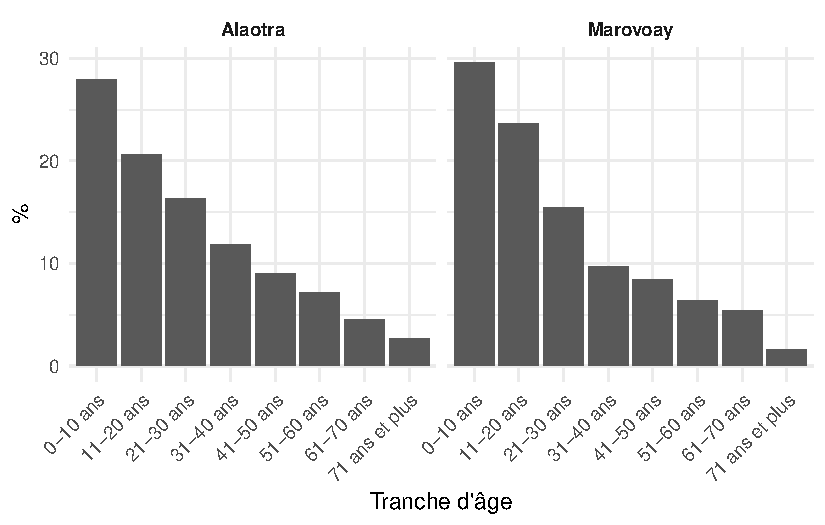
\includegraphics[keepaspectratio]{02_structure_menages_files/figure-pdf/fig_age_obs-1.pdf}}

}

\caption{Répartition des membres des ménages par tranche d'âge selon les
observatoires}

\end{figure}%

\begin{figure}[H]

{\centering \pandocbounded{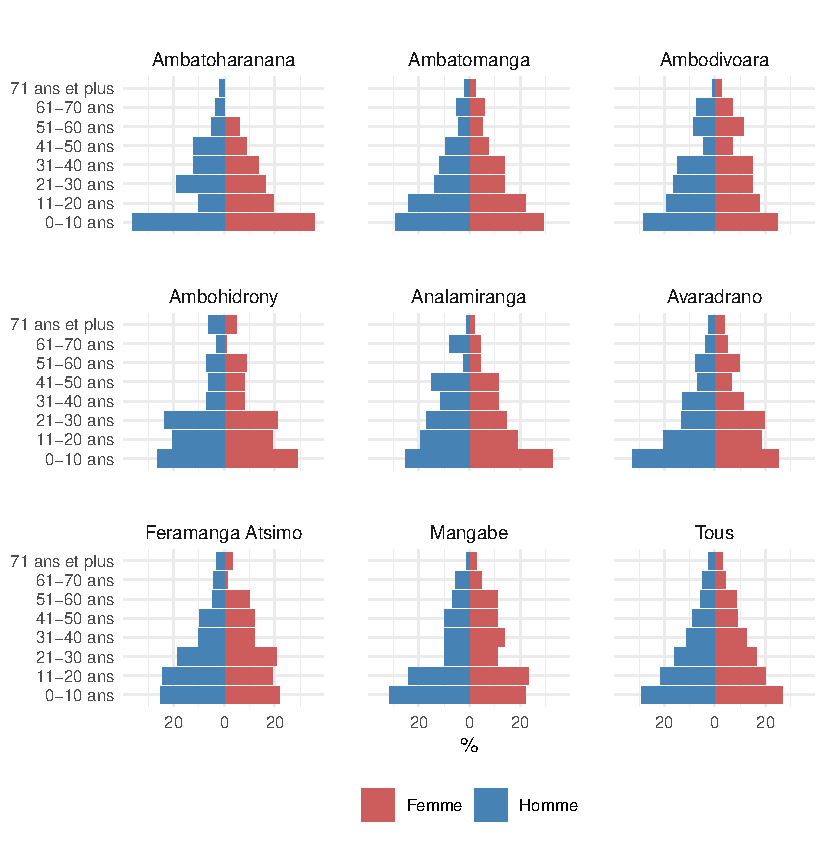
\includegraphics[keepaspectratio]{02_structure_menages_files/figure-pdf/fig_pyramide-1.pdf}}

}

\caption{Pyramide des âges des membres des ménages enquêtés par
observatoire}

\end{figure}%

\subsection{Origine des CM et
conjoints}\label{origine-des-cm-et-conjoints}

L'origine géographique des chefs de ménage et de leurs conjoints
renseigne sur les dynamiques migratoires et le degré d'ancrage local des
familles. La classification distingue les \emph{tompon-tany}
(autochtones), les \emph{zana-tany} (nés sur place de parents migrants),
les \emph{valivotaka} (migrants installés durablement) et les
\emph{mpihavy} (arrivants récents). La répartition de ces catégories
diffère sensiblement entre les deux observatoires.

\begin{table}
\caption*{
{\fontsize{20}{25}\selectfont  Origine des chefs de ménage et conjoints par observatoire\fontsize{12}{15}\selectfont } \\ 
{\fontsize{14}{17}\selectfont  Effectifs et pourcentages\fontsize{12}{15}\selectfont }
} 
\fontsize{12.0pt}{14.0pt}\selectfont
\begin{tabular*}{\linewidth}{@{\extracolsep{\fill}}lrrrr}
\toprule
 & \multicolumn{2}{c}{Chefs de ménage} & \multicolumn{2}{c}{Conjoints} \\ 
\cmidrule(lr){2-3} \cmidrule(lr){4-5}
Origine & N & \% & N & \% \\ 
\midrule\addlinespace[2.5pt]
\multicolumn{5}{l}{{\bfseries {Alaotra}}} \\[2.5pt] 
\midrule\addlinespace[2.5pt]
Mpihavy & 52 & 10.3 & 61 & 16.4 \\ 
Tompon-tany & 338 & 66.8 & 210 & 56.5 \\ 
Valivotaka & 26 & 5.1 & 28 & 7.5 \\ 
Zana-tany & 90 & 17.8 & 73 & 19.6 \\ 
\midrule\addlinespace[2.5pt]
\multicolumn{5}{l}{{\bfseries {Marovoay}}} \\[2.5pt] 
\midrule\addlinespace[2.5pt]
Mpihavy & 42 & 8.1 & 52 & 13.8 \\ 
Tompon-tany & 202 & 39.0 & 141 & 37.5 \\ 
Valivotaka & 70 & 13.5 & 43 & 11.4 \\ 
Zana-tany & 204 & 39.4 & 140 & 37.2 \\ 
\bottomrule
\end{tabular*}
\begin{minipage}{\linewidth}
\textbf{Source : Enquête auprès des OR 2025}\\
\end{minipage}
\end{table}

\pandocbounded{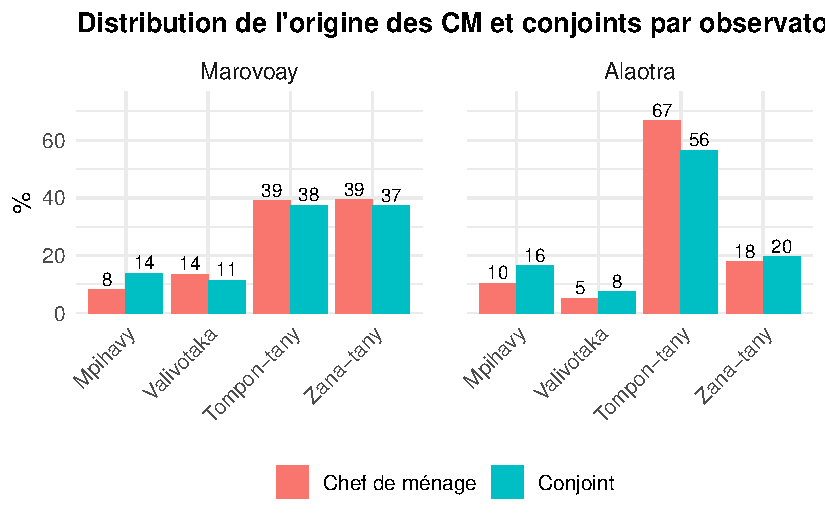
\includegraphics[keepaspectratio]{02_structure_menages_files/figure-pdf/fig_origine-1.pdf}}

\subsection{Région d'origine}\label{ruxe9gion-dorigine}

La provenance régionale des CM et conjoints qui ne sont pas natifs de la
localité permet d'identifier les principaux bassins migratoires
alimentant chaque observatoire.

\begin{table}
\caption*{
{\fontsize{20}{25}\selectfont  Région d'origine des CM et conjoints\fontsize{12}{15}\selectfont } \\ 
{\fontsize{14}{17}\selectfont  Effectifs et pourcentages\fontsize{12}{15}\selectfont }
} 
\fontsize{12.0pt}{14.0pt}\selectfont
\begin{tabular*}{\linewidth}{@{\extracolsep{\fill}}rrrrr}
\toprule
 & \multicolumn{2}{c}{Chefs de ménage} & \multicolumn{2}{c}{Conjoints} \\ 
\cmidrule(lr){2-3} \cmidrule(lr){4-5}
Région & N & \% & N & \% \\ 
\midrule\addlinespace[2.5pt]
\multicolumn{5}{l}{{\bfseries {Alaotra}}} \\[2.5pt] 
\midrule\addlinespace[2.5pt]
1 & 15 & 15.6 & 14 & 13.3 \\ 
2 & 21 & 21.9 & 34 & 32.4 \\ 
3 & 60 & 62.5 & 57 & 54.3 \\ 
\midrule\addlinespace[2.5pt]
\multicolumn{5}{l}{{\bfseries {Marovoay}}} \\[2.5pt] 
\midrule\addlinespace[2.5pt]
1 & 10 & 7.2 & 7 & 6.4 \\ 
2 & 5 & 3.6 & 21 & 19.1 \\ 
3 & 123 & 89.1 & 82 & 74.5 \\ 
\bottomrule
\end{tabular*}
\begin{minipage}{\linewidth}
\textbf{Source : Enquête auprès des OR 2025}\\
\end{minipage}
\end{table}

\pandocbounded{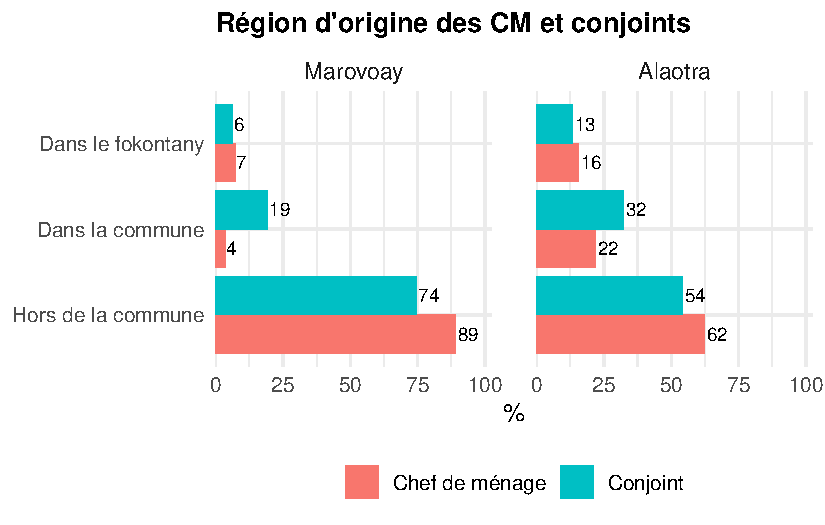
\includegraphics[keepaspectratio]{02_structure_menages_files/figure-pdf/fig_homeland-1.pdf}}

\subsection{Raison d'installation}\label{raison-dinstallation}

Les raisons d'installation des CM et conjoints non originaires du lieu
éclairent les motivations migratoires. Elles distinguent notamment les
installations liées au mariage de celles motivées par les opportunités
économiques (travail agricole ou non agricole).

\begin{table}
\caption*{
{\fontsize{20}{25}\selectfont  Raison d'implantation des CM et conjoints par observatoire\fontsize{12}{15}\selectfont } \\ 
{\fontsize{14}{17}\selectfont  Effectifs et pourcentages\fontsize{12}{15}\selectfont }
} 
\fontsize{12.0pt}{14.0pt}\selectfont
\begin{tabular*}{\linewidth}{@{\extracolsep{\fill}}lrrrr}
\toprule
 & \multicolumn{2}{c}{Chefs de ménage} & \multicolumn{2}{c}{Conjoints} \\ 
\cmidrule(lr){2-3} \cmidrule(lr){4-5}
Raison & N & \% & N & \% \\ 
\midrule\addlinespace[2.5pt]
\multicolumn{5}{l}{{\bfseries {Alaotra}}} \\[2.5pt] 
\midrule\addlinespace[2.5pt]
Autre raison & 0 & 0.0 & 0 & 0.0 \\ 
Mariage & 51 & 10.1 & 113 & 30.5 \\ 
Natif & 371 & 73.3 & 216 & 58.2 \\ 
Travail agricole & 46 & 9.1 & 25 & 6.7 \\ 
Travail non agricole & 35 & 6.9 & 15 & 4.0 \\ 
\midrule\addlinespace[2.5pt]
\multicolumn{5}{l}{{\bfseries {Marovoay}}} \\[2.5pt] 
\midrule\addlinespace[2.5pt]
Autre raison & 0 & 0.0 & 0 & 0.0 \\ 
Mariage & 19 & 3.7 & 82 & 21.8 \\ 
Natif & 373 & 71.9 & 234 & 62.2 \\ 
Travail agricole & 81 & 15.6 & 37 & 9.8 \\ 
Travail non agricole & 43 & 8.3 & 21 & 5.6 \\ 
\bottomrule
\end{tabular*}
\begin{minipage}{\linewidth}
\textbf{Source : Enquête auprès des OR 2025}\\
\end{minipage}
\end{table}

\pandocbounded{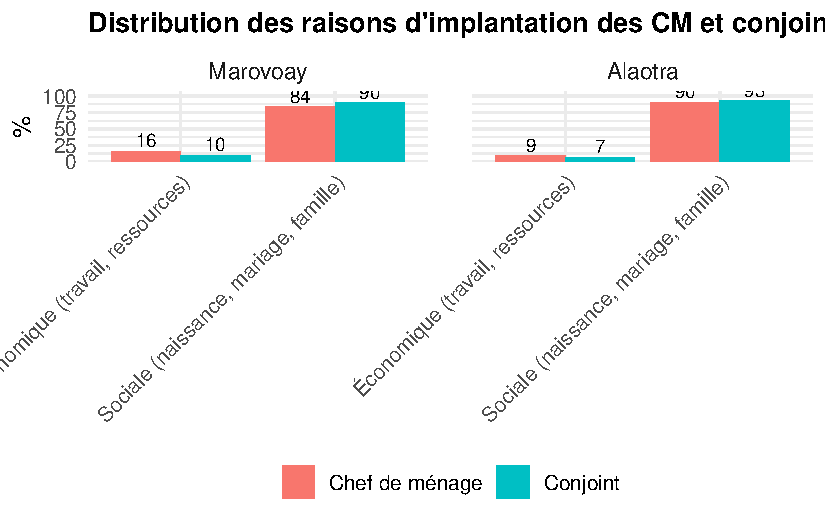
\includegraphics[keepaspectratio]{02_structure_menages_files/figure-pdf/fig_raison-1.pdf}}

\section{Caractéristiques des chefs de
ménages}\label{caractuxe9ristiques-des-chefs-de-muxe9nages}

Le profil des chefs de ménage (CM) est décrit ci-dessous.

\textbf{Alaotra.} 78.3 \% des CM sont des hommes, soit 21.7 \% de
ménages dirigés par des femmes. L'âge moyen des CM est de 45.4 ans. Sur
le plan conjugal, 74.2 \% des CM vivent en couple (mariés ou en
concubinage).

\textbf{Marovoay.} 78 \% des CM sont des hommes, soit 22 \% de ménages
dirigés par des femmes. L'âge moyen des CM est de 46.1 ans. Sur le plan
conjugal, 73 \% des CM vivent en couple (mariés ou en concubinage).

\subsection{Caractéristiques
socio-démographiques}\label{caractuxe9ristiques-socio-duxe9mographiques}

\begin{table}
\caption*{
{\fontsize{20}{25}\selectfont  Caractéristiques des chefs de ménage\textsuperscript{\textit{1}}\fontsize{12}{15}\selectfont }
} 
\fontsize{12.0pt}{14.0pt}\selectfont
\begin{tabular*}{\linewidth}{@{\extracolsep{\fill}}lrr}
\toprule
Catégorie & {\bfseries {Alaotra}} & {\bfseries {Marovoay}} \\ 
\midrule\addlinespace[2.5pt]
\multicolumn{3}{l}{{\bfseries {Sexe}}} \\[2.5pt] 
\midrule\addlinespace[2.5pt]
Femme & 110 (21.7\%) & 114 (22\%) \\ 
Homme & 397 (78.3\%) & 405 (78\%) \\ 
\midrule\addlinespace[2.5pt]
\multicolumn{3}{l}{{\bfseries {Âge}}} \\[2.5pt] 
\midrule\addlinespace[2.5pt]
Minimum & 16 & 18 \\ 
Mode & 27 & 36 \\ 
Médiane & 43 & 45 \\ 
Moyenne & 45 & 46 \\ 
Maximum & 90 & 96 \\ 
\midrule\addlinespace[2.5pt]
\multicolumn{3}{l}{{\bfseries {Statut matrimonial}}} \\[2.5pt] 
\midrule\addlinespace[2.5pt]
Célibataire & 2.2\% & 1.3\% \\ 
Divorcé(e) & 11\% & 16.2\% \\ 
En concubinage & 3.7\% & 6.2\% \\ 
Marié(e) civil / religieux / polygame & 20.9\% & 5.8\% \\ 
Marié(e) selon la tradition & 49.5\% & 61.1\% \\ 
Veuf(ve) & 12.6\% & 9.4\% \\ 
\bottomrule
\end{tabular*}
\begin{minipage}{\linewidth}
\textsuperscript{\textit{1}}Sexe et Statut matrimonial : effectifs et pourcentages. Âge : statistiques descriptives.\\
\textbf{Source : Enquête auprès des OR 2025}\\
\end{minipage}
\end{table}

\subsection{Niveau d'éducation}\label{niveau-duxe9ducation}

Le niveau d'éducation des chefs de ménage constitue un déterminant
majeur de la capacité d'adaptation et de la vulnérabilité des ménages
ruraux. L'analyse croisée par sexe met en évidence des disparités
supplémentaires.

\textbf{Alaotra.} Le niveau le plus fréquemment atteint est « Primaire »
(67.3 \% des CM).

\textbf{Marovoay.} Le niveau le plus fréquemment atteint est « Primaire
» (61 \% des CM).

\subsubsection{Niveau d'éducation du Chef de
ménage}\label{niveau-duxe9ducation-du-chef-de-muxe9nage}

\begin{table}
\caption*{
{\fontsize{20}{25}\selectfont  Répartition des chefs de ménage selon leur niveau d'éducation\fontsize{12}{15}\selectfont }
} 
\fontsize{12.0pt}{14.0pt}\selectfont
\begin{tabular*}{\linewidth}{@{\extracolsep{\fill}}lrr}
\toprule
Niveau d'éducation & {\bfseries {Alaotra}} & {\bfseries {Marovoay}} \\ 
\midrule\addlinespace[2.5pt]
Inconnu & 51 (10.1\%) & 78 (15\%) \\ 
Primaire & 307 (60.6\%) & 269 (51.8\%) \\ 
Secondaire 1er cycle & 109 (21.5\%) & 130 (25\%) \\ 
Secondaire 2ème cycle \& sup. & 40 (7.9\%) & 42 (8.1\%) \\ 
\bottomrule
\end{tabular*}
\begin{minipage}{\linewidth}
\textbf{Source : Enquête auprès des OR 2025}\\
\end{minipage}
\end{table}

\subsubsection{Niveau d'éducation des chefs de ménages par
sexe}\label{niveau-duxe9ducation-des-chefs-de-muxe9nages-par-sexe}

\begin{table}
\caption*{
{\fontsize{20}{25}\selectfont  Répartition des CM selon le niveau d'éducation et le sexe\textsuperscript{\textit{1}}\fontsize{12}{15}\selectfont }
} 
\fontsize{12.0pt}{14.0pt}\selectfont
\begin{tabular*}{\linewidth}{@{\extracolsep{\fill}}lrrrr}
\toprule
 & \multicolumn{2}{c}{Alaotra} & \multicolumn{2}{c}{Marovoay} \\ 
\cmidrule(lr){2-3} \cmidrule(lr){4-5}
Niveau d'éducation & Homme & Femme & Homme & Femme \\ 
\midrule\addlinespace[2.5pt]
Inconnu & 33 (8.3\%) & 18 (16.4\%) & 65 (16\%) & 13 (11.4\%) \\ 
Primaire & 237 (59.7\%) & 70 (63.6\%) & 199 (49.1\%) & 70 (61.4\%) \\ 
Secondaire 1er cycle & 92 (23.2\%) & 17 (15.5\%) & 104 (25.7\%) & 26 (22.8\%) \\ 
Secondaire 2ème cycle \& sup. & 35 (8.8\%) & 5 (4.5\%) & 37 (9.1\%) & 5 (4.4\%) \\ 
\bottomrule
\end{tabular*}
\begin{minipage}{\linewidth}
\textsuperscript{\textit{1}}Pourcentages calculés par rapport au total des CM de chaque sexe et observatoire.\\
\textbf{Source : Enquête auprès des OR 2025}\\
\end{minipage}
\end{table}

\subsection{Alphabétisation des chefs de
ménage}\label{alphabuxe9tisation-des-chefs-de-muxe9nage}

L'aptitude à lire et écrire conditionne l'accès à l'information, aux
services publics et aux opportunités économiques. Les sections suivantes
détaillent les compétences en lecture et en écriture séparément, avec
une ventilation par sexe.

\textbf{Alaotra.} 84.2 \% des CM savent lire et écrire.

\textbf{Marovoay.} 72.8 \% des CM savent lire et écrire.

\subsubsection{Savoir lire et écrire}\label{savoir-lire-et-uxe9crire}

\begin{table}
\caption*{
{\fontsize{20}{25}\selectfont  CM sachant lire et écrire\fontsize{12}{15}\selectfont }
} 
\fontsize{12.0pt}{14.0pt}\selectfont
\begin{tabular*}{\linewidth}{@{\extracolsep{\fill}}lr}
\toprule
Observatoire & Effectif \\ 
\midrule\addlinespace[2.5pt]
Alaotra & 427 \\ 
Marovoay & 378 \\ 
\bottomrule
\end{tabular*}
\begin{minipage}{\linewidth}
\textbf{Source : Enquête auprès des OR 2025}\\
\end{minipage}
\end{table}

\phantomsection\label{phngdbarcj}
CM sachant lire et écrire selon le sexe

Sexe

Effectif

\%

Alaotra

Femme

87

20.4

Homme

340

79.6

Marovoay

Femme

84

22.2

Homme

294

77.8

{{Source : Enquête auprès des OR 2025}}

\pandocbounded{
\includegraphics[keepaspectratio]{02_structure_menages_files/figure-pdf/cm_rw_sex-1.pdf}}\pandocbounded{
\includegraphics[keepaspectratio]{02_structure_menages_files/figure-pdf/cm_rw_sex-2.pdf}}

\subsubsection{Savoir lire}\label{savoir-lire}

\begin{table}
\caption*{
{\fontsize{20}{25}\selectfont  CM sachant lire\fontsize{12}{15}\selectfont }
} 
\fontsize{12.0pt}{14.0pt}\selectfont
\begin{tabular*}{\linewidth}{@{\extracolsep{\fill}}lr}
\toprule
Observatoire & Effectif \\ 
\midrule\addlinespace[2.5pt]
Alaotra & 428 \\ 
Marovoay & 384 \\ 
\bottomrule
\end{tabular*}
\begin{minipage}{\linewidth}
\textbf{Source : Enquête auprès des OR 2025}\\
\end{minipage}
\end{table}

\phantomsection\label{oxuxcmsbzw}
CM sachant lire selon le sexe

Sexe

Effectif

\%

Alaotra

Femme

87

20.3

Homme

341

79.7

Marovoay

Femme

85

22.1

Homme

299

77.9

{{Source : Enquête auprès des OR 2025}}

\pandocbounded{
\includegraphics[keepaspectratio]{02_structure_menages_files/figure-pdf/cm_r_sex-1.pdf}}\pandocbounded{
\includegraphics[keepaspectratio]{02_structure_menages_files/figure-pdf/cm_r_sex-2.pdf}}

\subsubsection{Savoir écrire}\label{savoir-uxe9crire}

\begin{table}
\caption*{
{\fontsize{20}{25}\selectfont  CM sachant écrire\fontsize{12}{15}\selectfont }
} 
\fontsize{12.0pt}{14.0pt}\selectfont
\begin{tabular*}{\linewidth}{@{\extracolsep{\fill}}lr}
\toprule
Observatoire & Effectif \\ 
\midrule\addlinespace[2.5pt]
Alaotra & 428 \\ 
Marovoay & 378 \\ 
\bottomrule
\end{tabular*}
\begin{minipage}{\linewidth}
\textbf{Source : Enquête auprès des OR 2025}\\
\end{minipage}
\end{table}

\phantomsection\label{ugfuqearau}
CM sachant écrire selon le sexe

Sexe

Effectif

\%

Alaotra

Femme

87

20.3

Homme

341

79.7

Marovoay

Femme

84

22.2

Homme

294

77.8

{{Source : Enquête auprès des OR 2025}}

\pandocbounded{
\includegraphics[keepaspectratio]{02_structure_menages_files/figure-pdf/cm_w_sex-1.pdf}}\pandocbounded{
\includegraphics[keepaspectratio]{02_structure_menages_files/figure-pdf/cm_w_sex-2.pdf}}

\subsection{Activités principales des Chefs de
ménage}\label{activituxe9s-principales-des-chefs-de-muxe9nage}

L'activité économique principale des chefs de ménage traduit la
structure productive de chaque observatoire. Les activités sont
regroupées en catégories sectorielles inspirées de la CITI Rév. 4 afin
de garantir un effectif suffisant dans chaque classe et de préserver la
confidentialité statistique.

\textbf{Alaotra.} L'activité dominante est « Cultivateur exploitant »
(60.4 \% des CM).

\textbf{Marovoay.} L'activité dominante est « Cultivateur exploitant »
(58.6 \% des CM).

\begin{table}
\caption*{
{\fontsize{20}{25}\selectfont  Activités principales du chef de ménage par observatoire\fontsize{12}{15}\selectfont }
} 
\fontsize{12.0pt}{14.0pt}\selectfont
\begin{tabular*}{\linewidth}{@{\extracolsep{\fill}}lrr}
\toprule
Activité & Effectif & \% \\ 
\midrule\addlinespace[2.5pt]
\multicolumn{3}{l}{{\bfseries {Alaotra}}} \\[2.5pt] 
\midrule\addlinespace[2.5pt]
Cultivateur exploitant & 305 & 60.4 \\ 
Ouvrier agricole & 63 & 12.5 \\ 
Artisanat, BTP \& Transport & 45 & 8.9 \\ 
Services \& Autres & 33 & 6.5 \\ 
Elevage, Pêche \& Ress. nat. & 31 & 6.1 \\ 
Commerce \& Restauration & 28 & 5.5 \\ 
\midrule\addlinespace[2.5pt]
\multicolumn{3}{l}{{\bfseries {Marovoay}}} \\[2.5pt] 
\midrule\addlinespace[2.5pt]
Cultivateur exploitant & 304 & 58.6 \\ 
Ouvrier agricole & 95 & 18.3 \\ 
Commerce \& Restauration & 38 & 7.3 \\ 
Artisanat, BTP \& Transport & 35 & 6.7 \\ 
Elevage, Pêche \& Ress. nat. & 25 & 4.8 \\ 
Services \& Autres & 22 & 4.2 \\ 
\bottomrule
\end{tabular*}
\begin{minipage}{\linewidth}
\textbf{Source : Enquête auprès des OR 2025}\\
\end{minipage}
\end{table}

\pandocbounded{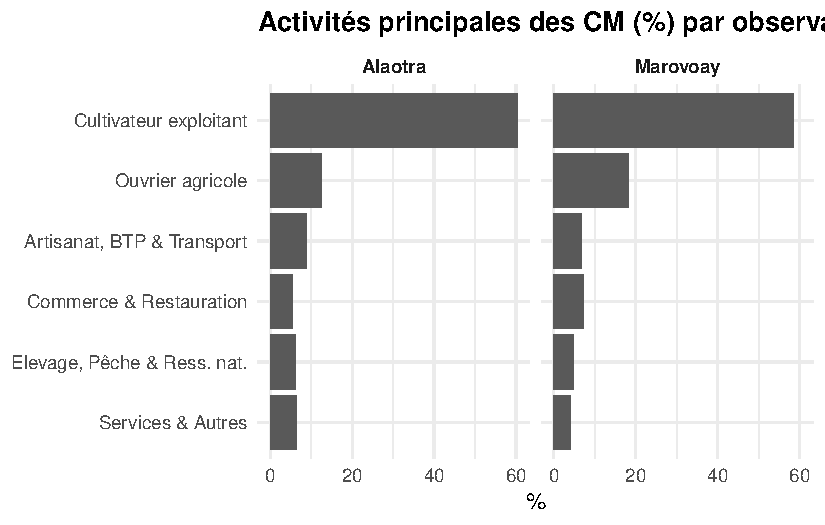
\includegraphics[keepaspectratio]{02_structure_menages_files/figure-pdf/cm_act-1.pdf}}

\subsubsection{Activités principales des CM par
sexe}\label{activituxe9s-principales-des-cm-par-sexe}

\begin{table}
\caption*{
{\fontsize{20}{25}\selectfont  Activités principales des CM par observatoire et sexe\fontsize{12}{15}\selectfont }
} 
\fontsize{12.0pt}{14.0pt}\selectfont
\begin{tabular*}{\linewidth}{@{\extracolsep{\fill}}lrrrr}
\toprule
 & \multicolumn{2}{c}{Femme} & \multicolumn{2}{c}{Homme} \\ 
\cmidrule(lr){2-3} \cmidrule(lr){4-5}
Activité & N & \% & N & \% \\ 
\midrule\addlinespace[2.5pt]
\multicolumn{5}{l}{{\bfseries {Alaotra}}} \\[2.5pt] 
\midrule\addlinespace[2.5pt]
Cultivateur exploitant & 46 & 42.2 & 259 & 65.4 \\ 
Commerce \& Restauration & 18 & 16.5 & 10 & 2.5 \\ 
Services \& Autres & 18 & 16.5 & 15 & 3.8 \\ 
Ouvrier agricole & 13 & 11.9 & 50 & 12.6 \\ 
Artisanat, BTP \& Transport & 8 & 7.3 & 37 & 9.3 \\ 
Elevage, Pêche \& Ress. nat. & 6 & 5.5 & 25 & 6.3 \\ 
\midrule\addlinespace[2.5pt]
\multicolumn{5}{l}{{\bfseries {Marovoay}}} \\[2.5pt] 
\midrule\addlinespace[2.5pt]
Cultivateur exploitant & 37 & 32.5 & 267 & 65.9 \\ 
Ouvrier agricole & 35 & 30.7 & 60 & 14.8 \\ 
Commerce \& Restauration & 26 & 22.8 & 12 & 3.0 \\ 
Services \& Autres & 8 & 7.0 & 14 & 3.5 \\ 
Elevage, Pêche \& Ress. nat. & 5 & 4.4 & 20 & 4.9 \\ 
Artisanat, BTP \& Transport & < 5 & < 5 & 32 & 7.9 \\ 
\bottomrule
\end{tabular*}
\begin{minipage}{\linewidth}
\textbf{Source : Enquête auprès des OR 2025}\\
\end{minipage}
\end{table}

\pandocbounded{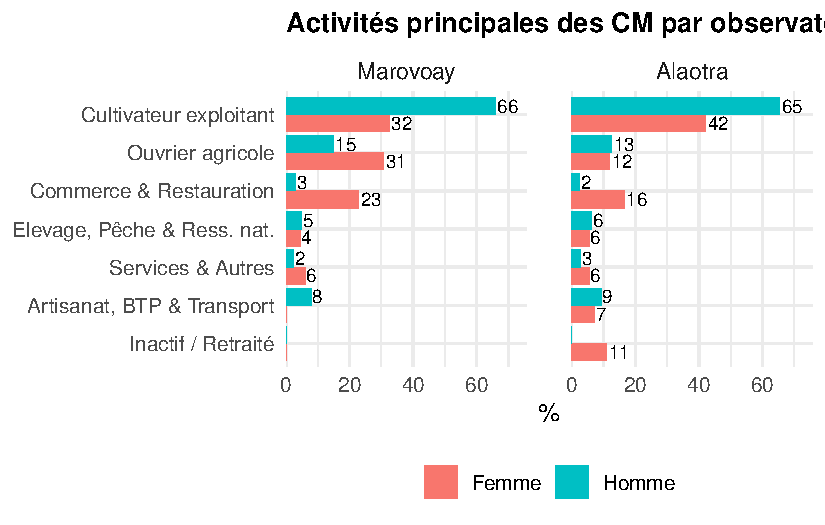
\includegraphics[keepaspectratio]{02_structure_menages_files/figure-pdf/cm_act_sex-1.pdf}}

\section{Caractéristiques des autres membres de
ménages}\label{caractuxe9ristiques-des-autres-membres-de-muxe9nages}

Les autres membres du ménage (conjoints, enfants, dépendants)
constituent la majorité de la population recensée. Leur profil
démographique, éducatif et économique complète celui des chefs de ménage
et permet de dresser un portrait plus complet du capital humain des
familles rurales.

\subsection{Caractéristiques
socio-démographiques}\label{caractuxe9ristiques-socio-duxe9mographiques-1}

\begin{table}
\caption*{
{\fontsize{20}{25}\selectfont  Caractéristiques des autres membres de ménage\textsuperscript{\textit{1}}\fontsize{12}{15}\selectfont }
} 
\fontsize{12.0pt}{14.0pt}\selectfont
\begin{tabular*}{\linewidth}{@{\extracolsep{\fill}}lrr}
\toprule
Catégorie & {\bfseries {Alaotra}} & {\bfseries {Marovoay}} \\ 
\midrule\addlinespace[2.5pt]
\multicolumn{3}{l}{{\bfseries {Sexe}}} \\[2.5pt] 
\midrule\addlinespace[2.5pt]
Femme & 877 (59.8\%) & 1046 (58.8\%) \\ 
Homme & 585 (39.9\%) & 730 (41.1\%) \\ 
NA & 5 (0.3\%) & 2 (0.1\%) \\ 
\midrule\addlinespace[2.5pt]
\multicolumn{3}{l}{{\bfseries {Âge}}} \\[2.5pt] 
\midrule\addlinespace[2.5pt]
Minimum & 0 & 0 \\ 
Mode & 0 & 12 \\ 
Médiane & 15 & 14 \\ 
Moyenne & 19 & 18 \\ 
Maximum & 93 & 99 \\ 
\midrule\addlinespace[2.5pt]
\multicolumn{3}{l}{{\bfseries {Statut matrimonial}}} \\[2.5pt] 
\midrule\addlinespace[2.5pt]
Célibataire & 38.2\% & 41.3\% \\ 
Divorcé(e) & 5\% & 6.8\% \\ 
En concubinage & 3.4\% & 5.5\% \\ 
Marié(e) civil / religieux / polygame & 14.9\% & 3.7\% \\ 
Marié(e) selon la tradition & 36.6\% & 40.3\% \\ 
Veuf(ve) & 2\% & 2.5\% \\ 
\bottomrule
\end{tabular*}
\begin{minipage}{\linewidth}
\textsuperscript{\textit{1}}Sexe et Statut matrimonial : effectifs et pourcentages. Âge : statistiques descriptives.\\
\textbf{Source : Enquête auprès des OR 2025}\\
\end{minipage}
\end{table}

\subsection{Éducation et
scolarisation}\label{uxe9ducation-et-scolarisation}

Le niveau d'éducation des autres membres de ménage complète le portrait
éducatif des familles. Les disparités entre sexes et entre observatoires
donnent un aperçu des inégalités d'accès à l'éducation.

\subsubsection{Niveau d'éducation des autres
membres}\label{niveau-duxe9ducation-des-autres-membres}

\begin{table}
\caption*{
{\fontsize{20}{25}\selectfont  Niveau d'éducation des autres membres de ménage\fontsize{12}{15}\selectfont }
} 
\fontsize{12.0pt}{14.0pt}\selectfont
\begin{tabular*}{\linewidth}{@{\extracolsep{\fill}}lrr}
\toprule
Niveau d'éducation & {\bfseries {Alaotra}} & {\bfseries {Marovoay}} \\ 
\midrule\addlinespace[2.5pt]
Inconnu & 356 (24.3\%) & 554 (31.2\%) \\ 
Primaire & 677 (46.1\%) & 854 (48\%) \\ 
Secondaire 1er cycle & 285 (19.4\%) & 256 (14.4\%) \\ 
Secondaire 2ème cycle \& sup. & 149 (10.2\%) & 114 (6.4\%) \\ 
\bottomrule
\end{tabular*}
\begin{minipage}{\linewidth}
\textbf{Source : Enquête auprès des OR 2025}\\
\end{minipage}
\end{table}

\subsubsection{Niveau d'éducation des autres membres par
sexe}\label{niveau-duxe9ducation-des-autres-membres-par-sexe}

\begin{table}
\caption*{
{\fontsize{20}{25}\selectfont  Niveau d'éducation des autres membres par sexe\fontsize{12}{15}\selectfont }
} 
\fontsize{12.0pt}{14.0pt}\selectfont
\begin{tabular*}{\linewidth}{@{\extracolsep{\fill}}lrrrr}
\toprule
 & \multicolumn{2}{c}{Alaotra} & \multicolumn{2}{c}{Marovoay} \\ 
\cmidrule(lr){2-3} \cmidrule(lr){4-5}
Niveau d'éducation & Homme & Femme & Homme & Femme \\ 
\midrule\addlinespace[2.5pt]
Inconnu & 174 (29.7\%) & 180 (20.5\%) & 272 (37.3\%) & 282 (27\%) \\ 
Primaire & 267 (45.6\%) & 407 (46.4\%) & 333 (45.6\%) & 521 (49.8\%) \\ 
Secondaire 1er cycle & 90 (15.4\%) & 195 (22.2\%) & 76 (10.4\%) & 179 (17.1\%) \\ 
Secondaire 2ème cycle \& sup. & 54 (9.2\%) & 95 (10.8\%) & 49 (6.7\%) & 64 (6.1\%) \\ 
\bottomrule
\end{tabular*}
\begin{minipage}{\linewidth}
\textbf{Source : Enquête auprès des OR 2025}\\
\end{minipage}
\end{table}

\subsubsection{Alphabétisation des autres
membres}\label{alphabuxe9tisation-des-autres-membres}

\paragraph{Savoir lire et écrire}\label{savoir-lire-et-uxe9crire-1}

\begin{table}
\caption*{
{\fontsize{20}{25}\selectfont  Autres membres sachant lire et écrire\fontsize{12}{15}\selectfont }
} 
\fontsize{12.0pt}{14.0pt}\selectfont
\begin{tabular*}{\linewidth}{@{\extracolsep{\fill}}lr}
\toprule
Observatoire & Effectif \\ 
\midrule\addlinespace[2.5pt]
Alaotra & 965 \\ 
Marovoay & 900 \\ 
\bottomrule
\end{tabular*}
\begin{minipage}{\linewidth}
\textbf{Source : Enquête auprès des OR 2025}\\
\end{minipage}
\end{table}

\phantomsection\label{snktgbzgas}
Autres membres sachant lire et écrire selon le sexe

Sexe

Effectif

\%

Alaotra

Femme

617

64.1

Homme

345

35.9

Marovoay

Femme

574

63.8

Homme

325

36.2

{{Source : Enquête auprès des OR 2025}}

\pandocbounded{
\includegraphics[keepaspectratio]{02_structure_menages_files/figure-pdf/other_rw_sex-1.pdf}}\pandocbounded{
\includegraphics[keepaspectratio]{02_structure_menages_files/figure-pdf/other_rw_sex-2.pdf}}

\paragraph{Savoir lire}\label{savoir-lire-1}

\begin{table}
\caption*{
{\fontsize{20}{25}\selectfont  Autres membres sachant lire\fontsize{12}{15}\selectfont }
} 
\fontsize{12.0pt}{14.0pt}\selectfont
\begin{tabular*}{\linewidth}{@{\extracolsep{\fill}}lr}
\toprule
Observatoire & Effectif \\ 
\midrule\addlinespace[2.5pt]
Alaotra & 971 \\ 
Marovoay & 902 \\ 
\bottomrule
\end{tabular*}
\begin{minipage}{\linewidth}
\textbf{Source : Enquête auprès des OR 2025}\\
\end{minipage}
\end{table}

\phantomsection\label{purpmhobxu}
Autres membres sachant lire selon le sexe

Sexe

Effectif

\%

Alaotra

Femme

620

64.0

Homme

348

36.0

Marovoay

Femme

576

63.9

Homme

325

36.1

{{Source : Enquête auprès des OR 2025}}

\pandocbounded{
\includegraphics[keepaspectratio]{02_structure_menages_files/figure-pdf/other_r_sex-1.pdf}}\pandocbounded{
\includegraphics[keepaspectratio]{02_structure_menages_files/figure-pdf/other_r_sex-2.pdf}}

\paragraph{Savoir écrire}\label{savoir-uxe9crire-1}

\begin{table}
\caption*{
{\fontsize{20}{25}\selectfont  Autres membres sachant écrire\fontsize{12}{15}\selectfont }
} 
\fontsize{12.0pt}{14.0pt}\selectfont
\begin{tabular*}{\linewidth}{@{\extracolsep{\fill}}lr}
\toprule
Observatoire & Effectif \\ 
\midrule\addlinespace[2.5pt]
Alaotra & 969 \\ 
Marovoay & 902 \\ 
\bottomrule
\end{tabular*}
\begin{minipage}{\linewidth}
\textbf{Source : Enquête auprès des OR 2025}\\
\end{minipage}
\end{table}

\phantomsection\label{dsfcfxvzqz}
Autres membres sachant écrire selon le sexe

Sexe

Effectif

\%

Alaotra

Femme

619

64.1

Homme

347

35.9

Marovoay

Femme

575

63.8

Homme

326

36.2

{{Source : Enquête auprès des OR 2025}}

\pandocbounded{
\includegraphics[keepaspectratio]{02_structure_menages_files/figure-pdf/other_w_sex-1.pdf}}\pandocbounded{
\includegraphics[keepaspectratio]{02_structure_menages_files/figure-pdf/other_w_sex-2.pdf}}

\subsection{Scolarisation}\label{scolarisation}

Le taux de scolarisation des enfants de 6 à 14 ans constitue un
indicateur clé du développement humain et de l'investissement des
ménages dans l'éducation.

\textbf{Alaotra.} Le taux de scolarisation s'élève à 93.7 \%.

\textbf{Marovoay.} Le taux de scolarisation s'élève à 81.7 \%.

\subsubsection{Taux de scolarisation des enfants de 6 à 14
ans}\label{taux-de-scolarisation-des-enfants-de-6-uxe0-14-ans}

\begin{table}
\caption*{
{\fontsize{20}{25}\selectfont  Taux de scolarisation des enfants de 6 à 14 ans\fontsize{12}{15}\selectfont }
} 
\fontsize{12.0pt}{14.0pt}\selectfont
\begin{tabular*}{\linewidth}{@{\extracolsep{\fill}}lrrrr}
\toprule
Observatoire & Non scolarisés (N) & Scolarisés (N) & Non scolarisés (\%) & Scolarisés (\%) \\ 
\midrule\addlinespace[2.5pt]
Alaotra & 26 & 387 & 6.3 & 93.7 \\ 
Marovoay & 111 & 497 & 18.3 & 81.7 \\ 
\bottomrule
\end{tabular*}
\begin{minipage}{\linewidth}
\textbf{Source : Enquête auprès des OR 2025}\\
\end{minipage}
\end{table}

\subsubsection{Classe suivie 2024-2025}\label{classe-suivie-2024-2025}

\begin{table}
\caption*{
{\fontsize{20}{25}\selectfont  Classe suivie en 2024-2025 par catégorie d'âge\fontsize{12}{15}\selectfont }
} 
\fontsize{12.0pt}{14.0pt}\selectfont
\begin{tabular*}{\linewidth}{@{\extracolsep{\fill}}lrrrr}
\toprule
Catégorie d'âge & {\bfseries {Primaire}} & {\bfseries {Secondaire 1er cycle}} & Secondaire 2ème cycle \& sup. & {\bfseries {Inconnu}} \\ 
\midrule\addlinespace[2.5pt]
\multicolumn{5}{l}{{\bfseries {Alaotra}}} \\[2.5pt] 
\midrule\addlinespace[2.5pt]
11-14 ans & 70.4 & 29.0 & 0.6 & 0.0 \\ 
15-17 ans & 49.5 & 41.2 & 9.3 & 0.0 \\ 
18-25 ans & 46.3 & 34.5 & 19.2 & 0.0 \\ 
3-5 ans & 43.6 & 2.6 & 53.8 & 0.0 \\ 
6-10 ans & 85.3 & 1.8 & 12.0 & 0.9 \\ 
\midrule\addlinespace[2.5pt]
\multicolumn{5}{l}{{\bfseries {Marovoay}}} \\[2.5pt] 
\midrule\addlinespace[2.5pt]
11-14 ans & 84.1 & 13.6 & 1.4 & 0.9 \\ 
15-17 ans & 58.5 & 36.6 & 4.9 & 0.0 \\ 
18-25 ans & 51.1 & 33.8 & 15.1 & 0.0 \\ 
3-5 ans & 44.4 & 0.0 & 51.9 & 3.7 \\ 
6-10 ans & 85.2 & 0.7 & 12.6 & 1.4 \\ 
\bottomrule
\end{tabular*}
\begin{minipage}{\linewidth}
\textbf{Source : Enquête auprès des OR 2025}\\
\end{minipage}
\end{table}

\subsubsection{Raisons de non fréquentation de l'école pour les 6 à 15
ans}\label{raisons-de-non-fruxe9quentation-de-luxe9cole-pour-les-6-uxe0-15-ans}

La Figure~\ref{fig-raisons-non-scol} et le
Table~\ref{tbl-raisons-non-scol} détaillent l'ensemble des motifs de
non-scolarisation cités.

\textbf{Alaotra.} Parmi les enfants de 6 à 15 ans non scolarisés, la
première raison invoquée est « Autre » (33.3 \%).

\textbf{Marovoay.} Parmi les enfants de 6 à 15 ans non scolarisés, la
première raison invoquée est « Frais trop élevés » (52.1 \%).

\begin{figure}

\centering{

\pandocbounded{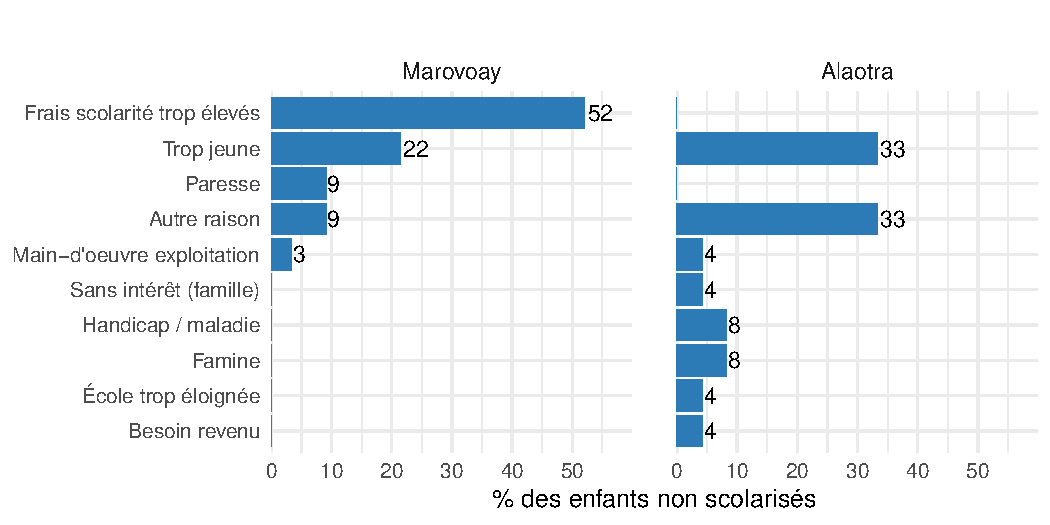
\includegraphics[keepaspectratio]{02_structure_menages_files/figure-pdf/fig-raisons-non-scol-1.pdf}}

}

\caption{\label{fig-raisons-non-scol}Principales raisons de
non-scolarisation ou d'arrêt des études (6-15 ans)}

\end{figure}%

\begin{table}

\caption{\label{tbl-raisons-non-scol}Raisons de non-scolarisation des
6-15 ans par observatoire}

\centering{

\caption*{
{\fontsize{20}{25}\selectfont  Raisons de non-fréquentation de l'école (6-15 ans)\fontsize{12}{15}\selectfont }
} 
\fontsize{12.0pt}{14.0pt}\selectfont
\begin{tabular*}{\linewidth}{@{\extracolsep{\fill}}lrr}
\toprule
Raison & Alaotra (\%) & Marovoay (\%) \\ 
\midrule\addlinespace[2.5pt]
Autre raison & 33.3 & 9.1 \\ 
Trop jeune & 33.3 & 21.5 \\ 
Famine & 8.3 & 0.0 \\ 
Handicap / maladie & 8.3 & 0.8 \\ 
Besoin revenu & 4.2 & 1.7 \\ 
Main-d'oeuvre exploitation & 4.2 & 3.3 \\ 
Sans intérêt (famille) & 4.2 & 0.0 \\ 
École trop éloignée & 4.2 & 0.8 \\ 
Autre & 0.0 & 1.7 \\ 
Frais scolarité trop élevés & 0.0 & 52.1 \\ 
Paresse & 0.0 & 9.1 \\ 
\bottomrule
\end{tabular*}

}

\end{table}%

\subsection{Activités principales des autres membres de
ménages}\label{activituxe9s-principales-des-autres-membres-de-muxe9nages}

La répartition sectorielle des activités des autres membres de ménage
reflète la diversification économique au sein des familles et le rôle
des conjoints et enfants dans l'économie du ménage. Les activités sont
regroupées selon la même nomenclature sectorielle que pour les CM.

\begin{table}
\caption*{
{\fontsize{20}{25}\selectfont  Activités principales des autres membres par observatoire\fontsize{12}{15}\selectfont }
} 
\fontsize{12.0pt}{14.0pt}\selectfont
\begin{tabular*}{\linewidth}{@{\extracolsep{\fill}}lrr}
\toprule
Activité & Effectif & \% \\ 
\midrule\addlinespace[2.5pt]
\multicolumn{3}{l}{{\bfseries {Alaotra}}} \\[2.5pt] 
\midrule\addlinespace[2.5pt]
Cultivateur exploitant & 391 & 52.9 \\ 
Services \& Autres & 84 & 11.4 \\ 
Ouvrier agricole & 76 & 10.3 \\ 
Commerce \& Restauration & 73 & 9.9 \\ 
Elève / Etudiant & 51 & 6.9 \\ 
Elevage, Pêche \& Ress. nat. & 35 & 4.7 \\ 
Artisanat, BTP \& Transport & 29 & 3.9 \\ 
\midrule\addlinespace[2.5pt]
\multicolumn{3}{l}{{\bfseries {Marovoay}}} \\[2.5pt] 
\midrule\addlinespace[2.5pt]
Cultivateur exploitant & 419 & 49.2 \\ 
Ouvrier agricole & 147 & 17.3 \\ 
Services \& Autres & 94 & 11.0 \\ 
Elève / Etudiant & 80 & 9.4 \\ 
Commerce \& Restauration & 64 & 7.5 \\ 
Artisanat, BTP \& Transport & 30 & 3.5 \\ 
Elevage, Pêche \& Ress. nat. & 18 & 2.1 \\ 
\bottomrule
\end{tabular*}
\begin{minipage}{\linewidth}
\textbf{Source : Enquête auprès des OR 2025}\\
\end{minipage}
\end{table}

\pandocbounded{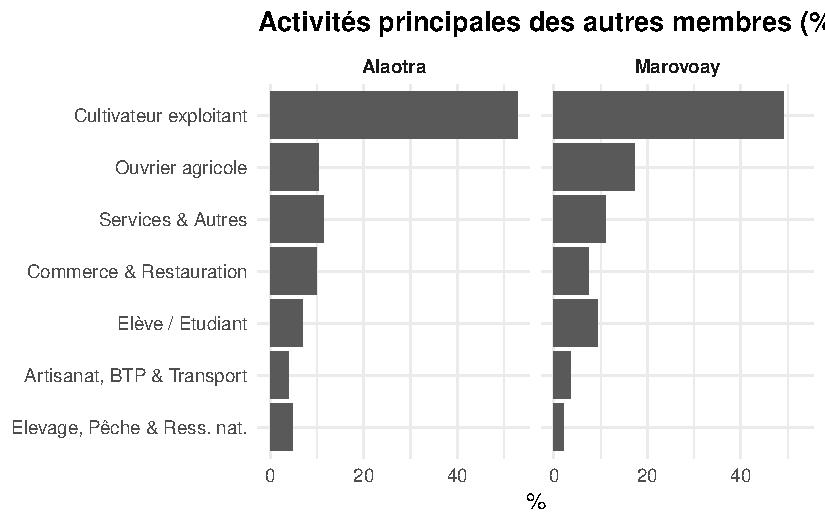
\includegraphics[keepaspectratio]{02_structure_menages_files/figure-pdf/other_act_grouped-1.pdf}}

\subsubsection{Activités principales des autres membres par
sexe}\label{activituxe9s-principales-des-autres-membres-par-sexe}

\begin{table}
\caption*{
{\fontsize{20}{25}\selectfont  Activités principales des autres membres par observatoire et sexe\fontsize{12}{15}\selectfont }
} 
\fontsize{12.0pt}{14.0pt}\selectfont
\begin{tabular*}{\linewidth}{@{\extracolsep{\fill}}lrrrr}
\toprule
 & \multicolumn{2}{c}{Femme} & \multicolumn{2}{c}{Homme} \\ 
\cmidrule(lr){2-3} \cmidrule(lr){4-5}
Activité & N & \% & N & \% \\ 
\midrule\addlinespace[2.5pt]
\multicolumn{5}{l}{{\bfseries {Alaotra}}} \\[2.5pt] 
\midrule\addlinespace[2.5pt]
Cultivateur exploitant & 289 & 54.9 & 101 & 47.6 \\ 
Commerce \& Restauration & 71 & 13.5 & < 5 & < 5 \\ 
Ouvrier agricole & 57 & 10.8 & 19 & 9.0 \\ 
Services \& Autres & 46 & 8.7 & 38 & 17.9 \\ 
Elève / Etudiant & 26 & 4.9 & 25 & 11.8 \\ 
Elevage, Pêche \& Ress. nat. & 19 & 3.6 & 16 & 7.5 \\ 
Artisanat, BTP \& Transport & 18 & 3.4 & 11 & 5.2 \\ 
\midrule\addlinespace[2.5pt]
\multicolumn{5}{l}{{\bfseries {Marovoay}}} \\[2.5pt] 
\midrule\addlinespace[2.5pt]
Cultivateur exploitant & 317 & 53.5 & 101 & 39.1 \\ 
Ouvrier agricole & 99 & 16.7 & 48 & 18.6 \\ 
Commerce \& Restauration & 60 & 10.1 & < 5 & < 5 \\ 
Services \& Autres & 57 & 9.6 & 37 & 14.3 \\ 
Elève / Etudiant & 34 & 5.7 & 46 & 17.8 \\ 
Artisanat, BTP \& Transport & 16 & 2.7 & 14 & 5.4 \\ 
Elevage, Pêche \& Ress. nat. & 10 & 1.7 & 8 & 3.1 \\ 
\bottomrule
\end{tabular*}
\begin{minipage}{\linewidth}
\textbf{Source : Enquête auprès des OR 2025}\\
\end{minipage}
\end{table}

\pandocbounded{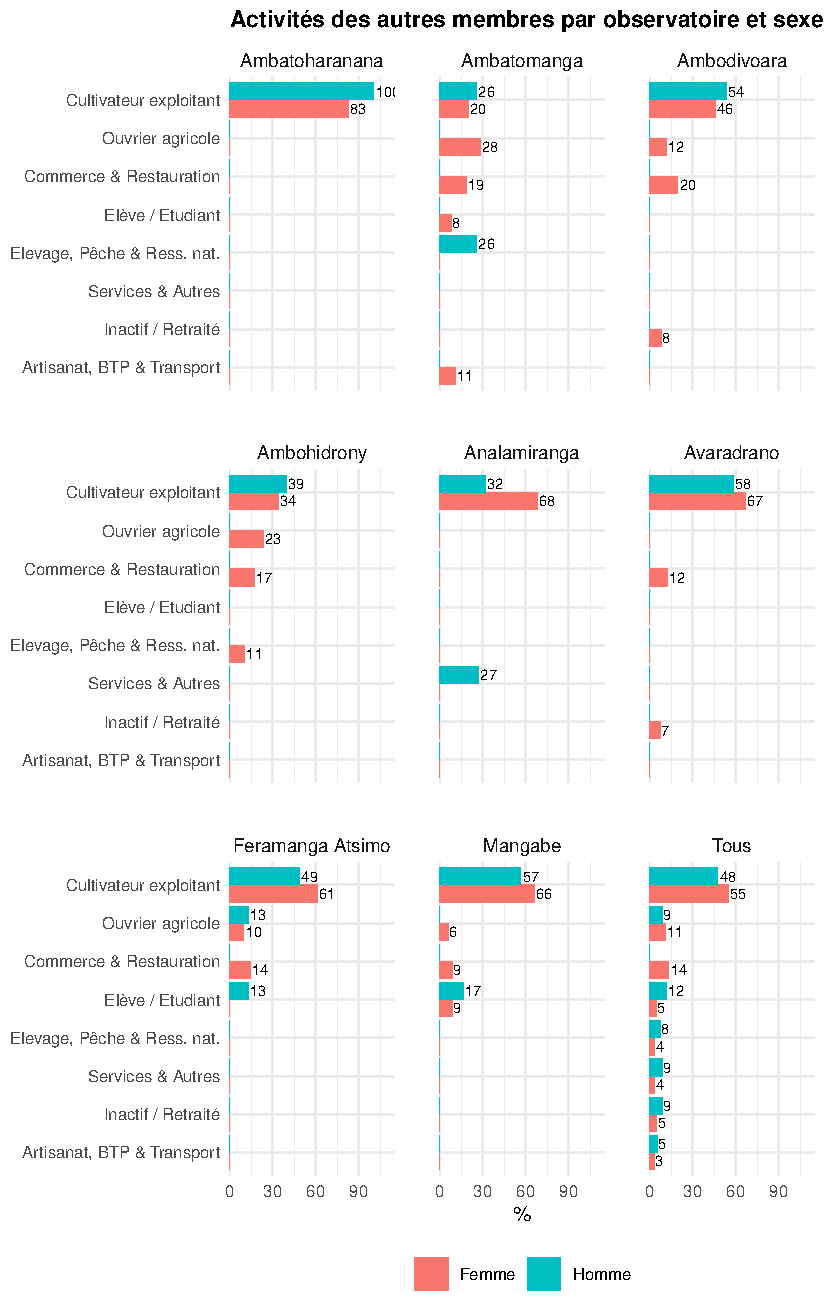
\includegraphics[keepaspectratio]{02_structure_menages_files/figure-pdf/other_act_sex-1.pdf}}

\section{Évolution des indicateurs démographiques
(1996-2025)}\label{sec-demog-multiyear}

Les observatoires d'Alaotra et de Marovoay disposent de données
démographiques depuis 1996. Cette section retrace l'évolution de quatre
indicateurs clés : la taille moyenne des ménages, la proportion de chefs
de ménage femmes, le taux de scolarisation des 6-14 ans et l'âge moyen
du chef de ménage.

\begin{tcolorbox}[enhanced jigsaw, colframe=quarto-callout-caution-color-frame, colback=white, titlerule=0mm, colbacktitle=quarto-callout-caution-color!10!white, toptitle=1mm, opacitybacktitle=0.6, title=\textcolor{quarto-callout-caution-color}{\faFire}\hspace{0.5em}{Interprétation : effet du panel et de l'échantillonnage}, left=2mm, leftrule=.75mm, bottomtitle=1mm, coltitle=black, arc=.35mm, rightrule=.15mm, bottomrule=.15mm, toprule=.15mm, opacityback=0, breakable]

Les tendances présentées dans cette section doivent être interprétées
avec prudence. Les observatoires suivaient un dispositif de
\textbf{panel} : la première année, les ménages sont tirés au sort dans
la localités, puis ils sont réinterrogés chaque année (avec remplacement
partiel si le ménage a disparu ou refuse de répondre). En 2025, après
dix ans d'interruption, un \textbf{nouveau tirage} a été effectué à
partir du dénombrement. Les évolutions observées reflètent donc à la
fois des dynamiques réelles dans les localités et des changements de
composition de l'échantillon (vieillissement du panel, attrition
sélective, renouvellement complet en 2025).

\end{tcolorbox}

\begin{figure}[H]

{\centering \pandocbounded{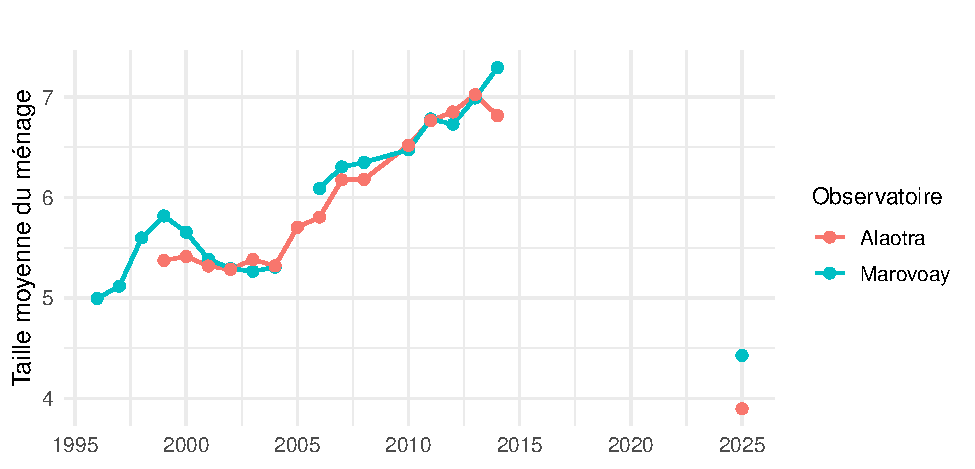
\includegraphics[keepaspectratio]{02_structure_menages_files/figure-pdf/fig_demog_taille-1.pdf}}

}

\caption{Évolution de la taille moyenne des ménages (1996-2025)}

\end{figure}%

\begin{figure}[H]

{\centering \pandocbounded{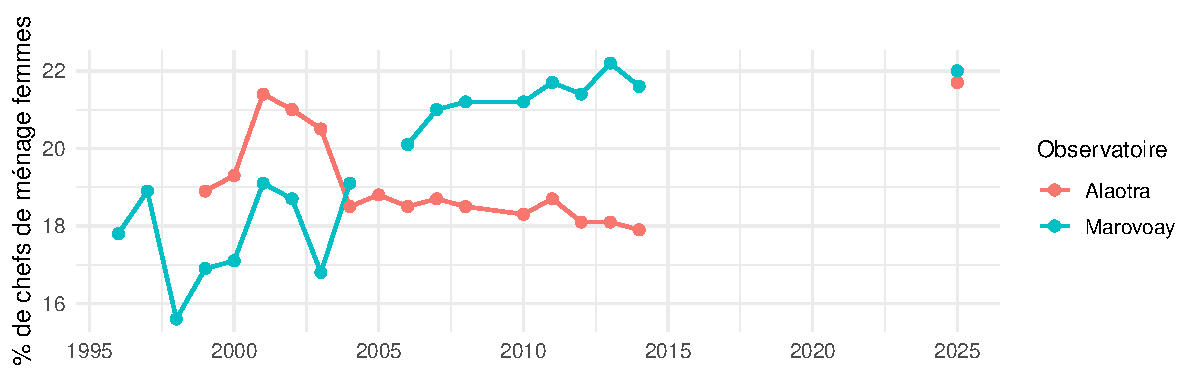
\includegraphics[keepaspectratio]{02_structure_menages_files/figure-pdf/fig_demog_fem_cm-1.pdf}}

}

\caption{Évolution du pourcentage de chefs de ménage femmes (1996-2025)}

\end{figure}%

\begin{figure}[H]

{\centering \pandocbounded{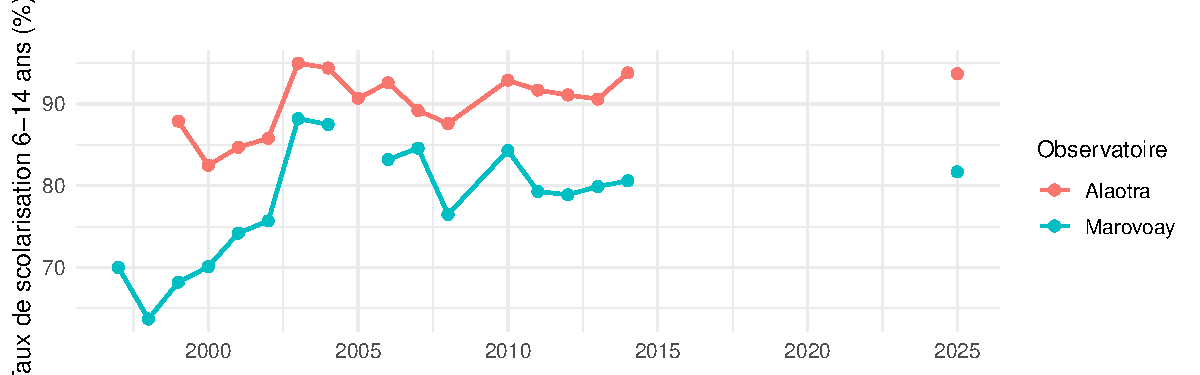
\includegraphics[keepaspectratio]{02_structure_menages_files/figure-pdf/fig_demog_scol-1.pdf}}

}

\caption{Évolution du taux de scolarisation des 6-14 ans (1996-2025)}

\end{figure}%

\begin{figure}[H]

{\centering \pandocbounded{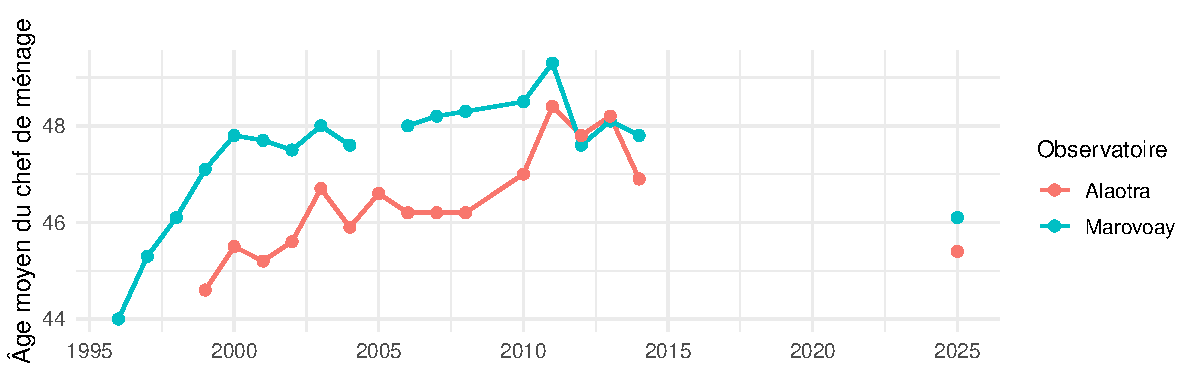
\includegraphics[keepaspectratio]{02_structure_menages_files/figure-pdf/fig_demog_age_cm-1.pdf}}

}

\caption{Évolution de l'âge moyen du chef de ménage (1996-2025)}

\end{figure}%

\bookmarksetup{startatroot}

\chapter{Habitat et niveau de vie}\label{habitat-et-niveau-de-vie}

Cette section decrit les conditions d'habitat, les equipements des
menages, leurs transferts et revenus.

\begin{tcolorbox}[enhanced jigsaw, colframe=quarto-callout-warning-color-frame, colback=white, titlerule=0mm, colbacktitle=quarto-callout-warning-color!10!white, toptitle=1mm, opacitybacktitle=0.6, title=\textcolor{quarto-callout-warning-color}{\faExclamationTriangle}\hspace{0.5em}{Travail de vérification en cours}, left=2mm, leftrule=.75mm, bottomtitle=1mm, coltitle=black, arc=.35mm, rightrule=.15mm, bottomrule=.15mm, toprule=.15mm, opacityback=0, breakable]

Les résultats présentés ci-dessous sont provisoires, et sont
susceptibles de faire l'objet de corrections.

\end{tcolorbox}

\textbf{Marovoay.} À Marovoay, les conditions d'habitat sont étroitement
liées à la position des ménages par rapport au fleuve Betsiboka. Les
fokontany de la rive droite (Bepako, Madiromiongana), situés en lisière
du Parc national d'Ankarafantsika, ont un accès plus limité aux
ressources en bois et matériaux de construction, notamment en raison des
restrictions liées à la conservation. L'approvisionnement en eau dépend
en grande partie du fleuve et de puits traditionnels. L'équipement
agricole y est dominé par les outils manuels, complétés par le recours à
la traction bovine pour le labour des rizières.

\textbf{Alaotra.} Dans l'Alaotra, les conditions d'habitat bénéficient
de la relative prospérité du premier bassin rizicole du pays. L'accès à
l'eau est facilité par la proximité du lac et du réseau d'irrigation,
mais la qualité de l'eau potable reste un enjeu sanitaire. Les ménages
des fokontany proches des périmètres irrigués (Avaradrano, Feramanga
Atsimo, Mangabe) disposent en moyenne d'un meilleur équipement agricole
que ceux des zones périphériques. La possession de biens de confort
courants y est plus répandue que dans d'autres observatoires ruraux de
Madagascar.

\section{Habitat}\label{habitat}

Les conditions d'habitat des ménages enquêtés témoignent des réalités du
milieu rural malgache. Le statut d'occupation, le type d'assainissement,
l'accès à l'eau, le mode d'éclairage et la source d'énergie de cuisson
constituent des indicateurs essentiels du cadre de vie.

\subsection{Statut d'occupation du
logement}\label{statut-doccupation-du-logement}

Le statut d'occupation du logement traduit la sécurité résidentielle des
ménages.

\textbf{Alaotra.} 74.2 \% des ménages occupent un logement en « En
propriété ».

\textbf{Marovoay.} 88.1 \% des ménages occupent un logement en « En
propriété ».

\begin{table}
\caption*{
{\fontsize{20}{25}\selectfont  Statut d'occupation du logement par observatoire\fontsize{12}{15}\selectfont }
} 
\fontsize{12.0pt}{14.0pt}\selectfont
\begin{tabular*}{\linewidth}{@{\extracolsep{\fill}}lrr}
\toprule
{\bfseries {Statut}} & N & \% \\ 
\midrule\addlinespace[2.5pt]
\multicolumn{3}{l}{{\bfseries {Alaotra}}} \\[2.5pt] 
\midrule\addlinespace[2.5pt]
En location & 51 & 10.1 \\ 
En propriété & 376 & 74.2 \\ 
Prêtée & 80 & 15.8 \\ 
\midrule\addlinespace[2.5pt]
\multicolumn{3}{l}{{\bfseries {Marovoay}}} \\[2.5pt] 
\midrule\addlinespace[2.5pt]
En location & 32 & 6.2 \\ 
En propriété & 457 & 88.1 \\ 
Prêtée & 30 & 5.8 \\ 
\bottomrule
\end{tabular*}
\begin{minipage}{\linewidth}
\textbf{Source : Enquête auprès des OR 2025}\\
\end{minipage}
\end{table}

\pandocbounded{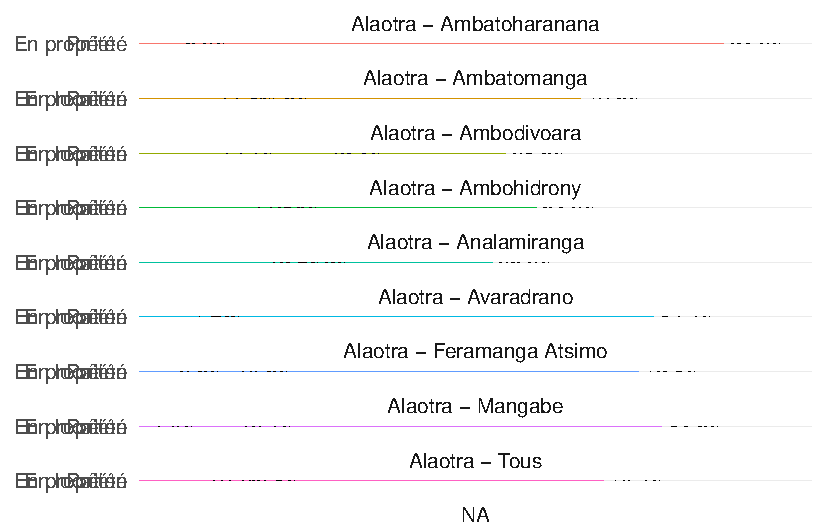
\includegraphics[keepaspectratio]{03_habitat_niveau_de_vie_files/figure-pdf/house_status-1.pdf}}

\subsection{Type de latrine}\label{type-de-latrine}

Le type de latrine constitue un indicateur sanitaire fondamental.

\textbf{Alaotra.} Le type dominant est « Fosse perdue en commun » (67.1
\% des ménages).

\textbf{Marovoay.} Le type dominant est « Dans la nature » (48.2 \% des
ménages).

\begin{table}
\caption*{
{\fontsize{20}{25}\selectfont  Types de latrine par observatoire\fontsize{12}{15}\selectfont }
} 
\fontsize{12.0pt}{14.0pt}\selectfont
\begin{tabular*}{\linewidth}{@{\extracolsep{\fill}}lrr}
\toprule
Type de latrine & N & \% \\ 
\midrule\addlinespace[2.5pt]
\multicolumn{3}{l}{{\bfseries {Alaotra}}} \\[2.5pt] 
\midrule\addlinespace[2.5pt]
Dans la nature & 35 & 6.9 \\ 
Fosse perdue en commun & 340 & 67.1 \\ 
Fosse perdue en individuel & 126 & 24.9 \\ 
Fosse septique en commun & 3 & 0.6 \\ 
Fosse septique en individuel & 3 & 0.6 \\ 
\midrule\addlinespace[2.5pt]
\multicolumn{3}{l}{{\bfseries {Marovoay}}} \\[2.5pt] 
\midrule\addlinespace[2.5pt]
Dans la nature & 250 & 48.2 \\ 
Fosse perdue en commun & 131 & 25.2 \\ 
Fosse perdue en individuel & 131 & 25.2 \\ 
Fosse septique en commun & 3 & 0.6 \\ 
Fosse septique en individuel & 4 & 0.8 \\ 
\bottomrule
\end{tabular*}
\begin{minipage}{\linewidth}
\textbf{Source : Enquête auprès des OR 2025}\\
\end{minipage}
\end{table}

\pandocbounded{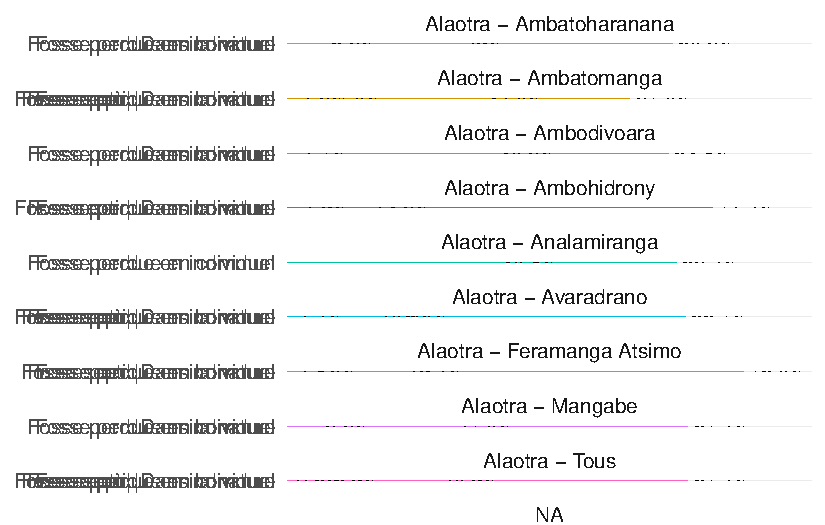
\includegraphics[keepaspectratio]{03_habitat_niveau_de_vie_files/figure-pdf/latrine-1.pdf}}

\subsection{Acces a l'eau}\label{acces-a-leau}

L'approvisionnement en eau détermine en grande partie les conditions
sanitaires des ménages ruraux.

\textbf{Alaotra.} La source principale est « Borne fontaine publique »
(54.8 \%).

\textbf{Marovoay.} La source principale est « Cours d?eau » (37.4 \%).

\begin{table}
\caption*{
{\fontsize{20}{25}\selectfont  Mode d'approvisionnement en eau par observatoire\fontsize{12}{15}\selectfont }
} 
\fontsize{12.0pt}{14.0pt}\selectfont
\begin{tabular*}{\linewidth}{@{\extracolsep{\fill}}lrr}
\toprule
Source & N & \% \\ 
\midrule\addlinespace[2.5pt]
\multicolumn{3}{l}{{\bfseries {Alaotra}}} \\[2.5pt] 
\midrule\addlinespace[2.5pt]
Autre \_\_\_\_\_\_\_\_\_\_\_\_\_\_\_\_\_\_\_\_\_\_\_\_\_\_\_\_ & 7 & 1.4 \\ 
Borne fontaine publique & 278 & 54.8 \\ 
Cours d?eau & 7 & 1.4 \\ 
Eau courante dans la maison/dans la cour & 8 & 1.6 \\ 
Puits (margelle) & 15 & 3.0 \\ 
Puits non aménagé (trou d?eau) & 159 & 31.4 \\ 
Source & 32 & 6.3 \\ 
NA & 1 & 0.2 \\ 
\midrule\addlinespace[2.5pt]
\multicolumn{3}{l}{{\bfseries {Marovoay}}} \\[2.5pt] 
\midrule\addlinespace[2.5pt]
Borne fontaine publique & 95 & 18.3 \\ 
Cours d?eau & 194 & 37.4 \\ 
Eau courante dans la maison/dans la cour & 4 & 0.8 \\ 
Impluvium & 1 & 0.2 \\ 
Puits (margelle) & 58 & 11.2 \\ 
Puits non aménagé (trou d?eau) & 143 & 27.6 \\ 
Source & 24 & 4.6 \\ 
\bottomrule
\end{tabular*}
\begin{minipage}{\linewidth}
\textbf{Source : Enquête auprès des OR 2025}\\
\end{minipage}
\end{table}

\pandocbounded{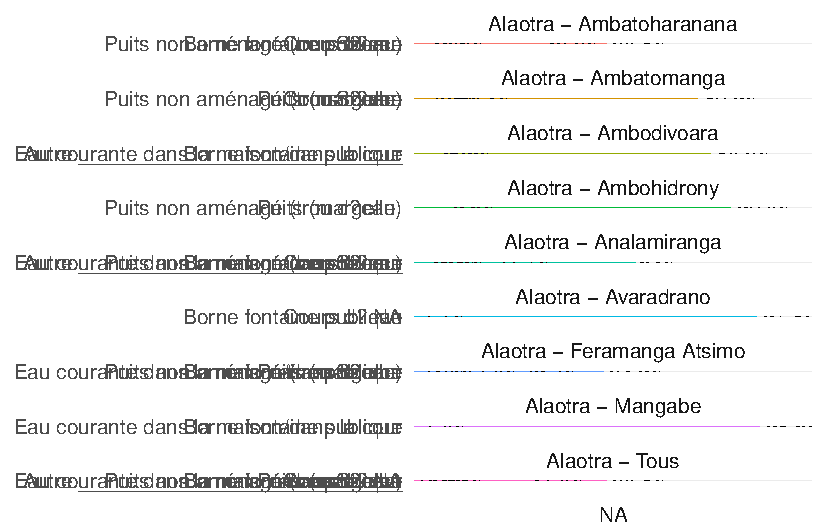
\includegraphics[keepaspectratio]{03_habitat_niveau_de_vie_files/figure-pdf/water-1.pdf}}

\subsection{Mode d'eclairage}\label{mode-declairage}

Le mode d'éclairage reflète le niveau d'accès à l'énergie moderne. Les
ménages ruraux dépendent encore largement de sources traditionnelles,
même si la pénétration du solaire progresse.

\begin{table}
\caption*{
{\fontsize{20}{25}\selectfont  Modes d'eclairage des menages par observatoire\fontsize{12}{15}\selectfont }
} 
\fontsize{12.0pt}{14.0pt}\selectfont
\begin{tabular*}{\linewidth}{@{\extracolsep{\fill}}lrr}
\toprule
Type d'eclairage & N & \% \\ 
\midrule\addlinespace[2.5pt]
\multicolumn{3}{l}{{\bfseries {Alaotra}}} \\[2.5pt] 
\midrule\addlinespace[2.5pt]
Batteries & 59 & 6.5 \\ 
Bois De Chauffe & 2 & 0.2 \\ 
Bougies & 22 & 2.4 \\ 
Electricité Réseau & 1 & 0.1 \\ 
Groupe Électrogène & 3 & 0.3 \\ 
Panneau Solaire En Marche ? & 232 & 25.4 \\ 
Piles & 63 & 6.9 \\ 
Pétrole Lampant & 290 & 31.8 \\ 
Solaire & 241 & 26.4 \\ 
\midrule\addlinespace[2.5pt]
\multicolumn{3}{l}{{\bfseries {Marovoay}}} \\[2.5pt] 
\midrule\addlinespace[2.5pt]
Autres & 31 & 3.6 \\ 
Batteries & 65 & 7.5 \\ 
Bois De Chauffe & 6 & 0.7 \\ 
Bougies & 4 & 0.5 \\ 
Panneau Solaire En Marche ? & 163 & 18.8 \\ 
Piles & 151 & 17.5 \\ 
Pétrole Lampant & 283 & 32.7 \\ 
Solaire & 162 & 18.7 \\ 
\bottomrule
\end{tabular*}
\begin{minipage}{\linewidth}
\textbf{Source : Enquête auprès des OR 2025}\\
\end{minipage}
\end{table}

\pandocbounded{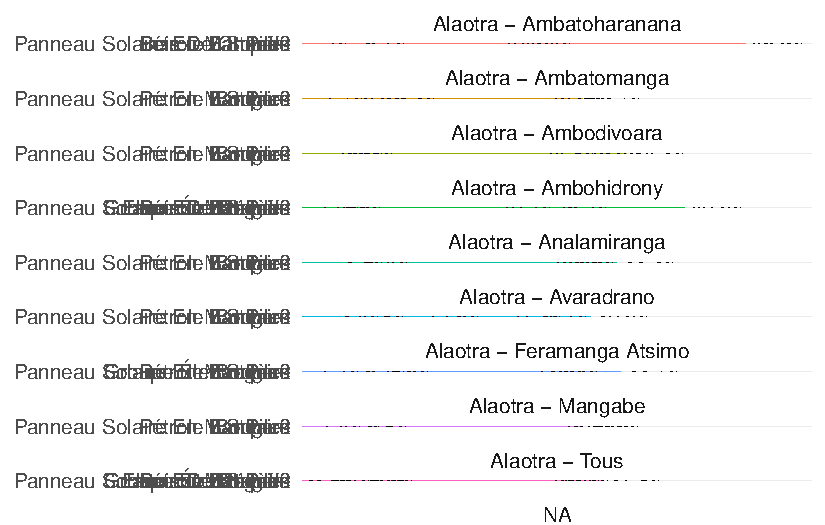
\includegraphics[keepaspectratio]{03_habitat_niveau_de_vie_files/figure-pdf/lighting-1.pdf}}

\subsection{Source d'energie pour la
cuisson}\label{source-denergie-pour-la-cuisson}

La quasi-totalité des ménages ruraux malgaches dépendent de la biomasse
pour la cuisson. La nature exacte du combustible utilisé (bois, charbon
de bois) varie selon la disponibilité locale des ressources forestières.

\begin{table}
\caption*{
{\fontsize{20}{25}\selectfont  Modes de cuisson des menages par observatoire\fontsize{12}{15}\selectfont }
} 
\fontsize{12.0pt}{14.0pt}\selectfont
\begin{tabular*}{\linewidth}{@{\extracolsep{\fill}}lrr}
\toprule
Source d'energie & N & \% \\ 
\midrule\addlinespace[2.5pt]
\multicolumn{3}{l}{{\bfseries {Alaotra}}} \\[2.5pt] 
\midrule\addlinespace[2.5pt]
Autre & 2 & 0.3 \\ 
Charbon & 218 & 34.0 \\ 
Gaz & 1 & 0.2 \\ 
Morceaux De Bois Résinés & 420 & 65.5 \\ 
\midrule\addlinespace[2.5pt]
\multicolumn{3}{l}{{\bfseries {Marovoay}}} \\[2.5pt] 
\midrule\addlinespace[2.5pt]
Charbon & 241 & 39.0 \\ 
Morceaux De Bois Résinés & 377 & 61.0 \\ 
\bottomrule
\end{tabular*}
\begin{minipage}{\linewidth}
\textbf{Source : Enquête auprès des OR 2025}\\
\end{minipage}
\end{table}

\pandocbounded{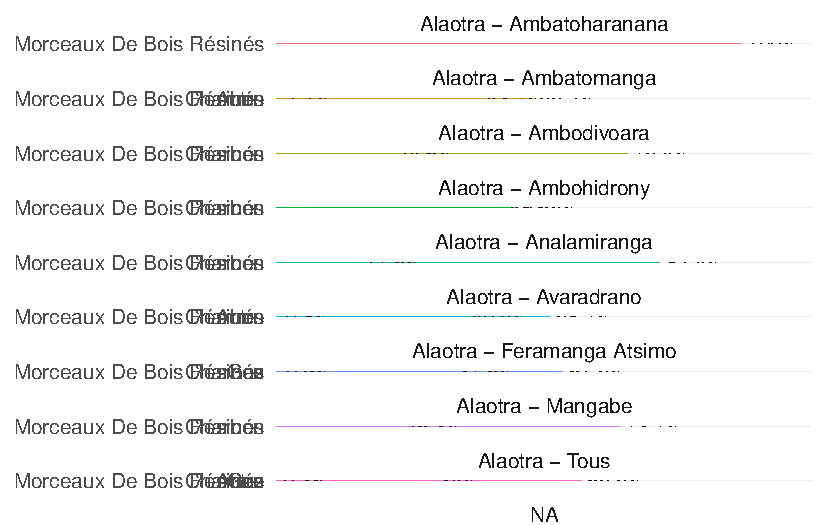
\includegraphics[keepaspectratio]{03_habitat_niveau_de_vie_files/figure-pdf/cooking-1.pdf}}

\section{Niveau de vie}\label{niveau-de-vie}

La possession de biens durables constitue un proxy classique du niveau
de vie des ménages en milieu rural, où les revenus monétaires sont
souvent difficiles à mesurer.

\subsection{Biens de confort courant}\label{biens-de-confort-courant}

Les biens de confort courant (mobilier, ustensiles, outils) renseignent
sur le niveau d'équipement quotidien des ménages et constituent un
indicateur de bien-être matériel.

\begin{table}
\caption*{
{\fontsize{20}{25}\selectfont  Taux de possession de biens de confort courants\fontsize{12}{15}\selectfont }
} 
\fontsize{12.0pt}{14.0pt}\selectfont
\begin{tabular*}{\linewidth}{@{\extracolsep{\fill}}lrr}
\toprule
Bien & N & \% \\ 
\midrule\addlinespace[2.5pt]
\multicolumn{3}{l}{{\bfseries {Alaotra}}} \\[2.5pt] 
\midrule\addlinespace[2.5pt]
Antenne Parabolique ( Canal+ Parabole Startimes & 15 & 1.1 \\ 
Bicyclette & 184 & 12.9 \\ 
Chaises & 56 & 3.9 \\ 
Lecteur Vcd / Dvd / Divx & 39 & 2.7 \\ 
Lits & 229 & 16.0 \\ 
Marmites & 8 & 0.6 \\ 
Moto & 27 & 1.9 \\ 
Nattes Pour Dormir & 102 & 7.1 \\ 
Radio / Radio-K7 & 264 & 18.5 \\ 
Tables & 235 & 16.5 \\ 
Téléphone Fixe Ou Mobile & 190 & 13.3 \\ 
Télévision & 77 & 5.4 \\ 
Voiture/Camionnette & 2 & 0.1 \\ 
\midrule\addlinespace[2.5pt]
\multicolumn{3}{l}{{\bfseries {Marovoay}}} \\[2.5pt] 
\midrule\addlinespace[2.5pt]
Antenne Parabolique ( Canal+ Parabole Startimes & 16 & 1.2 \\ 
Bicyclette & 40 & 3.1 \\ 
Chaises & 34 & 2.7 \\ 
Lecteur Vcd / Dvd / Divx & 5 & 0.4 \\ 
Lits & 263 & 20.5 \\ 
Marmites & 3 & 0.2 \\ 
Moto & 7 & 0.5 \\ 
Nattes Pour Dormir & 199 & 15.5 \\ 
Radio / Radio-K7 & 224 & 17.5 \\ 
Tables & 224 & 17.5 \\ 
Téléphone Fixe Ou Mobile & 237 & 18.5 \\ 
Télévision & 27 & 2.1 \\ 
Voiture/Camionnette & 3 & 0.2 \\ 
\bottomrule
\end{tabular*}
\begin{minipage}{\linewidth}
\textbf{Source : Enquête auprès des OR 2025}\\
\end{minipage}
\end{table}

\pandocbounded{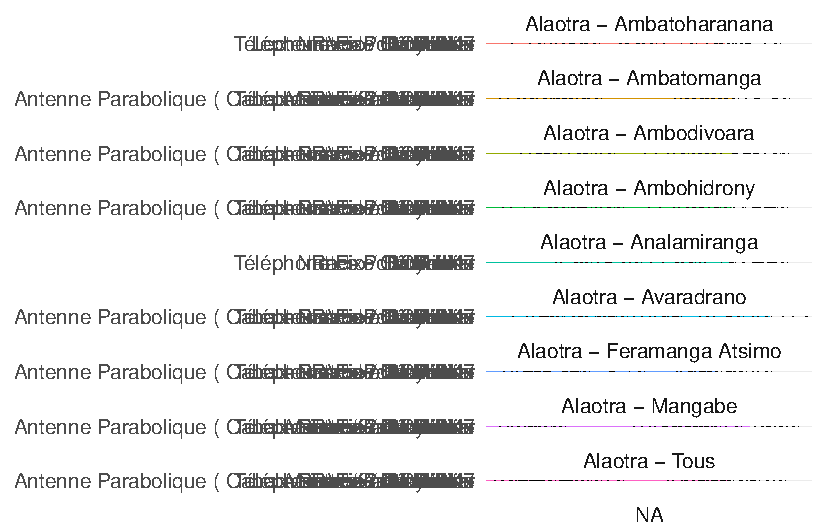
\includegraphics[keepaspectratio]{03_habitat_niveau_de_vie_files/figure-pdf/comfort_goods-1.pdf}}

\subsection{Equipement agricole}\label{equipement-agricole}

L'équipement agricole conditionne la productivité et la capacité
d'extension des surfaces cultivées. La possession de matériel mécanisé
ou de traction animale constitue un facteur de différenciation important
entre les ménages.

\begin{table}
\caption*{
{\fontsize{20}{25}\selectfont  Taux de possession d'equipements agricoles\fontsize{12}{15}\selectfont }
} 
\fontsize{12.0pt}{14.0pt}\selectfont
\begin{tabular*}{\linewidth}{@{\extracolsep{\fill}}lrrr}
\toprule
{\bfseries {Equipement}} & Menages (N) & Menages (\%) & Nb outils \\ 
\midrule\addlinespace[2.5pt]
\multicolumn{4}{l}{{\bfseries {Alaotra}}} \\[2.5pt] 
\midrule\addlinespace[2.5pt]
 & 460 & 90.7 & 5,088 \\ 
Angady & 442 & 87.2 & 456 \\ 
Faucille/Coupe-coupe & 270 & 53.3 & 334 \\ 
Arrosoir/Sceau & 165 & 32.5 & 194 \\ 
Râteau, fourche & 91 & 17.9 & 94 \\ 
Hache & 77 & 15.2 & 77 \\ 
Couteau & 46 & 9.1 & 47 \\ 
Pulvérisateur & 46 & 9.1 & 46 \\ 
Charrue & 41 & 8.1 & 41 \\ 
Pompe hydraulique & 27 & 5.3 & 27 \\ 
Herse/Pulvériseur/Rotovat & 24 & 4.7 & 24 \\ 
Sarcleuse & 24 & 4.7 & 24 \\ 
Motoculteur, type Kubota & 22 & 4.3 & 22 \\ 
Bœuf (ex : piétinage) & 17 & 3.4 & 17 \\ 
Natte et semblables (goel & 11 & 2.2 & 11 \\ 
Bidon (genre bidon à pétr & 8 & 1.6 & 8 \\ 
Pioche & 8 & 1.6 & 8 \\ 
Nasse & 7 & 1.4 & 7 \\ 
Hafa & 6 & 1.2 & 8 \\ 
Tracteur & 6 & 1.2 & 7 \\ 
Bicyclette & 4 & 0.8 & 4 \\ 
Scie & 4 & 0.8 & 4 \\ 
Autres & 3 & 0.6 & 3 \\ 
Barre à mine & 3 & 0.6 & 3 \\ 
Charrette attelée (à trac & 3 & 0.6 & 3 \\ 
Egreneuse & 3 & 0.6 & 3 \\ 
Semoir attelé & 3 & 0.6 & 3 \\ 
Brouette & 2 & 0.4 & 2 \\ 
Soubique, produits de tis & 2 & 0.4 & 2 \\ 
Camion & 1 & 0.2 & 1 \\ 
Charrette non attelée (à & 1 & 0.2 & 1 \\ 
Rouleau & 1 & 0.2 & 1 \\ 
\midrule\addlinespace[2.5pt]
\multicolumn{4}{l}{{\bfseries {Marovoay}}} \\[2.5pt] 
\midrule\addlinespace[2.5pt]
 & 435 & 83.8 & 4,776 \\ 
Angady & 425 & 81.9 & 425 \\ 
Faucille/Coupe-coupe & 314 & 60.5 & 447 \\ 
Hache & 133 & 25.6 & 133 \\ 
Charrue & 122 & 23.5 & 122 \\ 
Couteau & 114 & 22.0 & 123 \\ 
Herse/Pulvériseur/Rotovat & 105 & 20.2 & 105 \\ 
Bœuf (ex : piétinage) & 64 & 12.3 & 64 \\ 
Charrette attelée (à trac & 39 & 7.5 & 39 \\ 
Natte et semblables (goel & 33 & 6.4 & 33 \\ 
Soubique, produits de tis & 24 & 4.6 & 24 \\ 
Bidon (genre bidon à pétr & 14 & 2.7 & 14 \\ 
Houe & 12 & 2.3 & 12 \\ 
Arrosoir/Sceau & 10 & 1.9 & 10 \\ 
Filet & 5 & 1.0 & 5 \\ 
Sarcleuse & 5 & 1.0 & 5 \\ 
Motoculteur, type Kubota & 4 & 0.8 & 4 \\ 
Rouleau & 4 & 0.8 & 4 \\ 
Barre à mine & 3 & 0.6 & 3 \\ 
Brouette & 3 & 0.6 & 3 \\ 
Hafa & 3 & 0.6 & 4 \\ 
Pulvérisateur & 3 & 0.6 & 3 \\ 
Râteau, fourche & 3 & 0.6 & 4 \\ 
Canne planteuse & 2 & 0.4 & 2 \\ 
Corde (ex : servant pour & 2 & 0.4 & 2 \\ 
Tracteur & 2 & 0.4 & 2 \\ 
Balance & 1 & 0.2 & 1 \\ 
Camion & 1 & 0.2 & 1 \\ 
Décortiqueur / dépailleur & 1 & 0.2 & 1 \\ 
Pompe hydraulique & 1 & 0.2 & 1 \\ 
Scie & 1 & 0.2 & 1 \\ 
\bottomrule
\end{tabular*}
\begin{minipage}{\linewidth}
\textbf{Source : Enquête auprès des OR 2025}\\
\end{minipage}
\end{table}

\pandocbounded{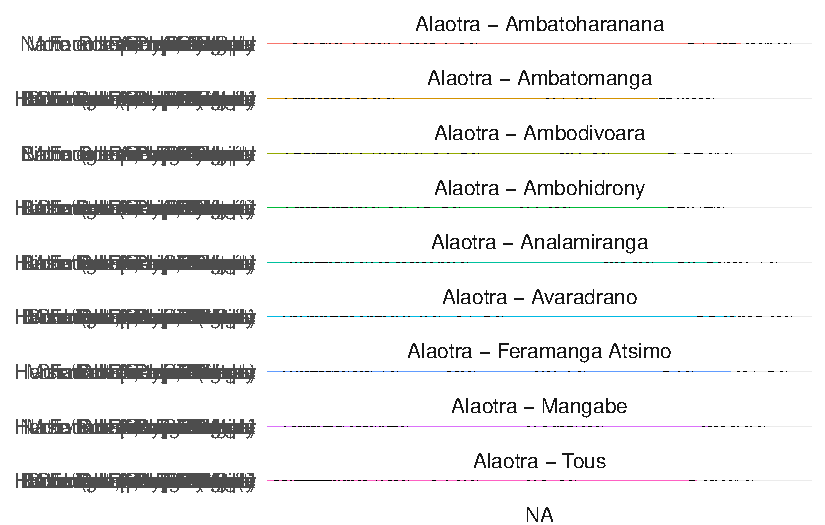
\includegraphics[keepaspectratio]{03_habitat_niveau_de_vie_files/figure-pdf/agri_equipment-1.pdf}}

\subsection{Materiel de communication audiovisuelle et
telecommunication}\label{materiel-de-communication-audiovisuelle-et-telecommunication}

L'accès aux technologies de communication et d'information constitue un
vecteur de connexion aux marchés, aux services et à l'information. La
pénétration du téléphone mobile a transformé les pratiques économiques
et sociales en milieu rural.

\begin{table}
\caption*{
{\fontsize{20}{25}\selectfont  Materiels de communication audiovisuelle et telecommunication\fontsize{12}{15}\selectfont }
} 
\fontsize{12.0pt}{14.0pt}\selectfont
\begin{tabular*}{\linewidth}{@{\extracolsep{\fill}}lrr}
\toprule
Equipement & N & \% \\ 
\midrule\addlinespace[2.5pt]
\multicolumn{3}{l}{{\bfseries {Alaotra}}} \\[2.5pt] 
\midrule\addlinespace[2.5pt]
Antenne Parabolique ( Canal+ Parabole Startimes & 15 & 2.6 \\ 
Lecteur Vcd / Dvd / Divx & 39 & 6.7 \\ 
Radio / Radio-K7 & 264 & 45.1 \\ 
Téléphone Fixe Ou Mobile & 190 & 32.5 \\ 
Télévision & 77 & 13.2 \\ 
\midrule\addlinespace[2.5pt]
\multicolumn{3}{l}{{\bfseries {Marovoay}}} \\[2.5pt] 
\midrule\addlinespace[2.5pt]
Antenne Parabolique ( Canal+ Parabole Startimes & 16 & 3.1 \\ 
Lecteur Vcd / Dvd / Divx & 5 & 1.0 \\ 
Radio / Radio-K7 & 224 & 44.0 \\ 
Téléphone Fixe Ou Mobile & 237 & 46.6 \\ 
Télévision & 27 & 5.3 \\ 
\bottomrule
\end{tabular*}
\begin{minipage}{\linewidth}
\textbf{Source : Enquête auprès des OR 2025}\\
\end{minipage}
\end{table}

\pandocbounded{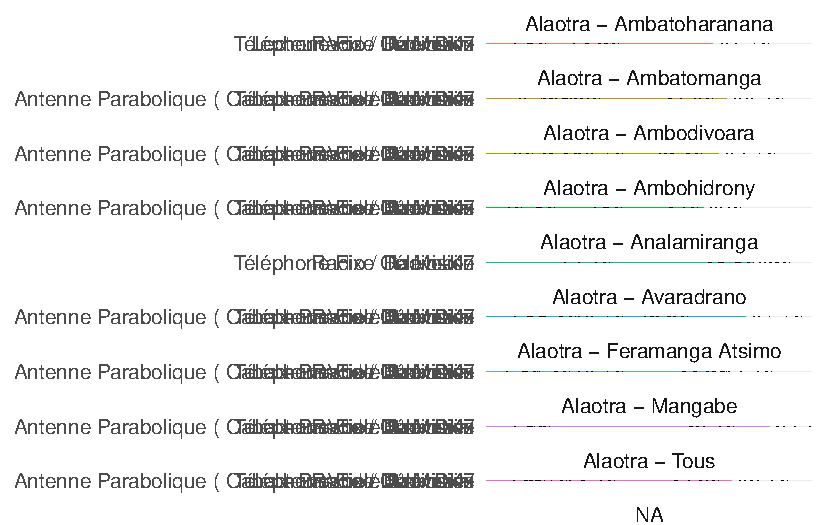
\includegraphics[keepaspectratio]{03_habitat_niveau_de_vie_files/figure-pdf/communication-1.pdf}}

\section{Transferts sortants}\label{transferts-sortants}

Le fichier \texttt{res\_t2} recense les transferts envoyes par les
menages a des personnes exterieures au foyer. Chaque ligne correspond a
un destinataire. Les variables cles sont le type de transfert
(\texttt{t21a}), le lieu de residence du destinataire (\texttt{t41}), le
poids de riz envoye (\texttt{t42}, en kg) et la valeur totale
(\texttt{t21d}, en Ar).

\begin{figure}

\centering{

\pandocbounded{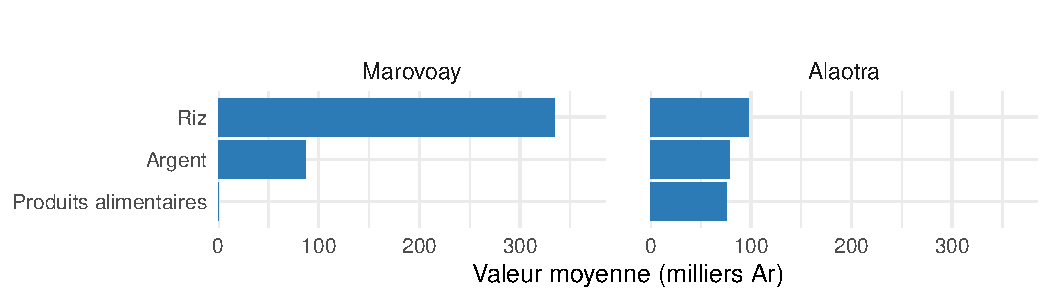
\includegraphics[keepaspectratio]{03_habitat_niveau_de_vie_files/figure-pdf/fig-transferts-sortants-1.pdf}}

}

\caption{\label{fig-transferts-sortants}Valeur moyenne des transferts
sortants par observatoire et type}

\end{figure}%

\begin{table}

\caption{\label{tbl-transferts-sortants}Transferts sortants : resume par
observatoire}

\centering{

\caption*{
{\fontsize{20}{25}\selectfont  Menages envoyant des transferts\fontsize{12}{15}\selectfont }
} 
\fontsize{12.0pt}{14.0pt}\selectfont
\begin{tabular*}{\linewidth}{@{\extracolsep{\fill}}lrrr}
\toprule
{\bfseries {Observatory}} & Nb envoyeurs & Nb menages total & \% envoyeurs \\ 
\midrule\addlinespace[2.5pt]
Alaotra & 507 & 507 & 100 \\ 
Marovoay & 519 & 519 & 100 \\ 
\bottomrule
\end{tabular*}
\begin{minipage}{\linewidth}
\textbf{Source : Enquête auprès des OR 2025}\\
\end{minipage}

}

\end{table}%

\begin{figure}

\centering{

\pandocbounded{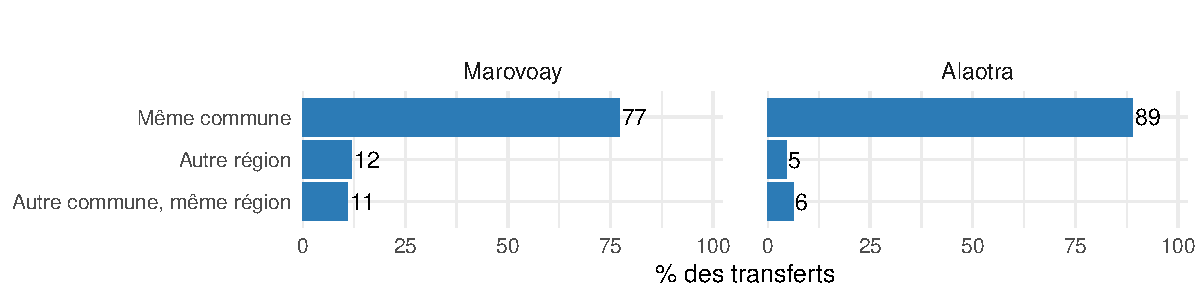
\includegraphics[keepaspectratio]{03_habitat_niveau_de_vie_files/figure-pdf/fig-destination-transferts-1.pdf}}

}

\caption{\label{fig-destination-transferts}Lieu de residence des
destinataires de transferts}

\end{figure}%

\section{Revenu}\label{revenu}

Les revenus presentes ici sont des revenus annuels par menage, calcules
sur la periode de reference (PR) de la campagne 2025. Le revenu total
(\texttt{revtot}) se decompose en revenu courant (\texttt{revcou}) et
revenu exceptionnel (\texttt{revexcept}).

Le revenu courant agrege sept composantes :

\begin{itemize}
\tightlist
\item
  les \textbf{salaires agricoles} (\texttt{revsec}) : remuneration du
  travail salarie agricole ;
\item
  les \textbf{salaires non-agricoles} (\texttt{revppal}) : remuneration
  du travail salarie hors agriculture ;
\item
  les \textbf{revenus independants} (\texttt{rev\_indep}) : revenus des
  activites liberales et artisanales non-agricoles ;
\item
  le \textbf{revenu net rizicole} (\texttt{rev\_riz}) : valeur de la
  production de riz moins les charges ;
\item
  le \textbf{revenu net des autres cultures} (\texttt{rev\_cu}) : meme
  logique pour les cultures non-rizicoles ;
\item
  le \textbf{revenu de l'elevage} (\texttt{revel}) : ventes d'animaux et
  produits d'elevage ;
\item
  la \textbf{peche} (\texttt{revpeche}).
\end{itemize}

Le revenu exceptionnel regroupe les rentes foncieres, les autres
revenus, le travail HIMO, la decapitalisation et les transferts recus.

\subsection{Structure du revenu total}\label{structure-du-revenu-total}

Le revenu total annuel par ménage synthétise l'ensemble des ressources
monétaires et non-monétaires. Les écarts entre moyenne et médiane
reflètent le degré d'inégalité au sein de chaque observatoire.

\begin{table}
\caption*{
{\fontsize{20}{25}\selectfont  Revenu total annuel par menage et par observatoire (Ar/an)\fontsize{12}{15}\selectfont } \\ 
{\fontsize{14}{17}\selectfont  Campagne 2025\fontsize{12}{15}\selectfont }
} 
\fontsize{12.0pt}{14.0pt}\selectfont
\begin{tabular*}{\linewidth}{@{\extracolsep{\fill}}lrrrrrr}
\toprule
{\bfseries {Observatory}} & {\bfseries {Nb menages}} & {\bfseries {Moyenne}} & {\bfseries {Mediane}} & {\bfseries {Ecart-type}} & {\bfseries {Minimum}} & {\bfseries {Maximum}} \\ 
\midrule\addlinespace[2.5pt]
Alaotra & 507 & 4,488,029 & 2,692,468 & 10,312,760 & -7,244,963 & 171,961,683 \\ 
Marovoay & 519 & 3,480,646 & 2,094,749 & 5,475,598 & -4,219,928 & 72,641,968 \\ 
\bottomrule
\end{tabular*}
\begin{minipage}{\linewidth}
\textbf{Source : Enquête auprès des OR 2025}\\
\end{minipage}
\end{table}

\subsection{Decomposition du revenu
courant}\label{decomposition-du-revenu-courant}

La décomposition du revenu courant en ses sept composantes met en
lumière la structure productive de chaque observatoire et le degré de
dépendance à l'égard de la riziculture.

\begin{table}
\caption*{
{\fontsize{20}{25}\selectfont  Decomposition du revenu courant moyen par menage (Ar/an)\fontsize{12}{15}\selectfont } \\ 
{\fontsize{14}{17}\selectfont  Campagne 2025\fontsize{12}{15}\selectfont }
} 
\fontsize{12.0pt}{14.0pt}\selectfont
\begin{tabular*}{\linewidth}{@{\extracolsep{\fill}}lrrrr}
\toprule
{\bfseries {Composante}} & {\bfseries {Alaotra}} & {\bfseries {Marovoay}} & Alaotra (\%) & Marovoay (\%) \\ 
\midrule\addlinespace[2.5pt]
Salaires agricoles & 860,748 & 604,846 & 19.8 & 18.4 \\ 
Salaires non-agricoles & 297,052 & 204,131 & 6.8 & 6.2 \\ 
Revenus independants & 1,043,037 & 759,874 & 24.0 & 23.2 \\ 
Revenu net rizicole & 1,654,368 & 1,287,310 & 38.0 & 39.2 \\ 
Revenu net autres cultures & 191,317 & 170,901 & 4.4 & 5.2 \\ 
Elevage & 302,735 & 253,697 & 7.0 & 7.7 \\ 
Peche & 0 & 0 & 0.0 & 0.0 \\ 
{\bfseries Total revenu courant} & {\bfseries 4,349,257} & {\bfseries 3,280,758} & {\bfseries 100.0} & {\bfseries 100.0} \\ 
\bottomrule
\end{tabular*}
\begin{minipage}{\linewidth}
\textbf{Source : Enquête auprès des OR 2025}\\
\end{minipage}
\end{table}

\begin{figure}[H]

{\centering \pandocbounded{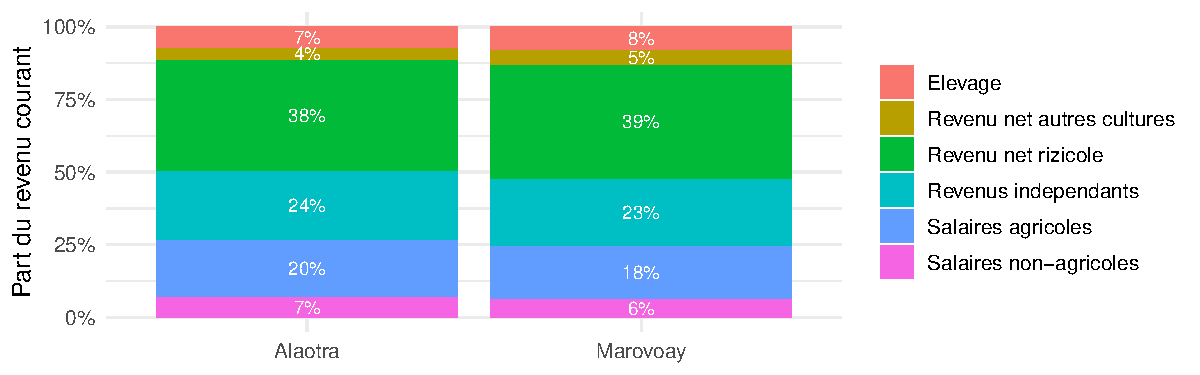
\includegraphics[keepaspectratio]{03_habitat_niveau_de_vie_files/figure-pdf/fig_revcou_shares-1.pdf}}

}

\caption{Part des composantes dans le revenu courant moyen par
observatoire}

\end{figure}%

\subsection{Distribution du revenu
total}\label{distribution-du-revenu-total}

La distribution du revenu total illustre le degré d'inégalité au sein de
chaque observatoire. L'utilisation d'une échelle logarithmique permet de
mieux visualiser l'étalement de la distribution et la concentration des
ménages à bas revenus.

\begin{figure}[H]

{\centering \pandocbounded{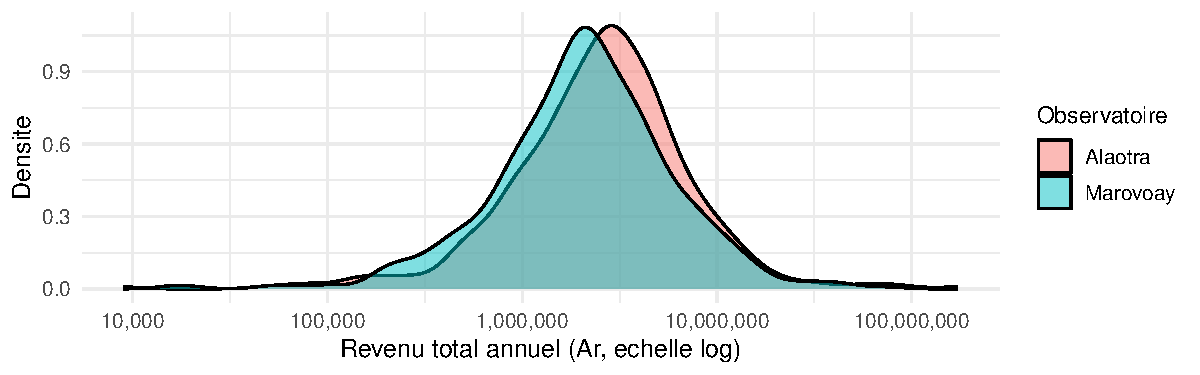
\includegraphics[keepaspectratio]{03_habitat_niveau_de_vie_files/figure-pdf/fig_revtot_dist-1.pdf}}

}

\caption{Distribution du revenu total par observatoire (echelle log)}

\end{figure}%

\subsection{Revenu courant et revenu
exceptionnel}\label{revenu-courant-et-revenu-exceptionnel}

La distinction entre revenu courant (activités régulières) et revenu
exceptionnel (transferts, décapitalisation, travaux HIMO) renseigne sur
la durabilité des ressources des ménages. Un poids élevé du revenu
exceptionnel peut signaler une vulnérabilité économique.

\begin{table}
\caption*{
{\fontsize{20}{25}\selectfont  Revenu courant et revenu exceptionnel moyens par menage (Ar/an)\fontsize{12}{15}\selectfont } \\ 
{\fontsize{14}{17}\selectfont  Campagne 2025\fontsize{12}{15}\selectfont }
} 
\fontsize{12.0pt}{14.0pt}\selectfont
\begin{tabular*}{\linewidth}{@{\extracolsep{\fill}}lrrrr}
\toprule
{\bfseries {Observatory}} & {\bfseries {Revenu courant}} & {\bfseries {Revenu exceptionnel}} & {\bfseries {Revenu total}} & Part courant (\%) \\ 
\midrule\addlinespace[2.5pt]
Alaotra & 4,349,257 & 138,771 & 4,488,029 & 96.9 \\ 
Marovoay & 3,280,758 & 199,888 & 3,480,646 & 94.3 \\ 
\bottomrule
\end{tabular*}
\begin{minipage}{\linewidth}
\textbf{Source : Enquête auprès des OR 2025}\\
\end{minipage}
\end{table}

\subsection{Menages a revenu negatif ou
nul}\label{menages-a-revenu-negatif-ou-nul}

Certains menages presentent un revenu courant negatif, principalement en
raison de charges agricoles superieures aux produits (mauvaises
recoltes, couts d'intrants eleves).

\begin{table}
\caption*{
{\fontsize{20}{25}\selectfont  Menages a revenu courant ou total negatif ou nul\fontsize{12}{15}\selectfont }
} 
\fontsize{12.0pt}{14.0pt}\selectfont
\begin{tabular*}{\linewidth}{@{\extracolsep{\fill}}lrrrr}
\toprule
{\bfseries {Observatory}} & {\bfseries {Nb menages}} & {\bfseries {Revenu courant <= 0}} & \% <= 0 & {\bfseries {Revenu total <= 0}} \\ 
\midrule\addlinespace[2.5pt]
Alaotra & 507 & 10 & 2.0 & 5 \\ 
Marovoay & 519 & 10 & 1.9 & 5 \\ 
\bottomrule
\end{tabular*}
\begin{minipage}{\linewidth}
\textbf{Source : Enquête auprès des OR 2025}\\
\end{minipage}
\end{table}

\section{Evolution des revenus nominaux depuis
1995}\label{sec-income-multiyear}

Les observatoires de Marovoay et d'Alaotra disposent de series longues
permettant de suivre l'evolution des revenus sur trois decennies. Les
donnees couvrent 1995-2008 et 2010-2014 pour Marovoay, 1999-2008 et
2010-2014 pour Alaotra, ainsi que la campagne 2025 pour les deux. Les
annees 2009 et 2015-2024 ne contiennent pas ces observatoires. Le trait
pointille materialise l'absence de donnees.

\begin{figure}[H]

{\centering \pandocbounded{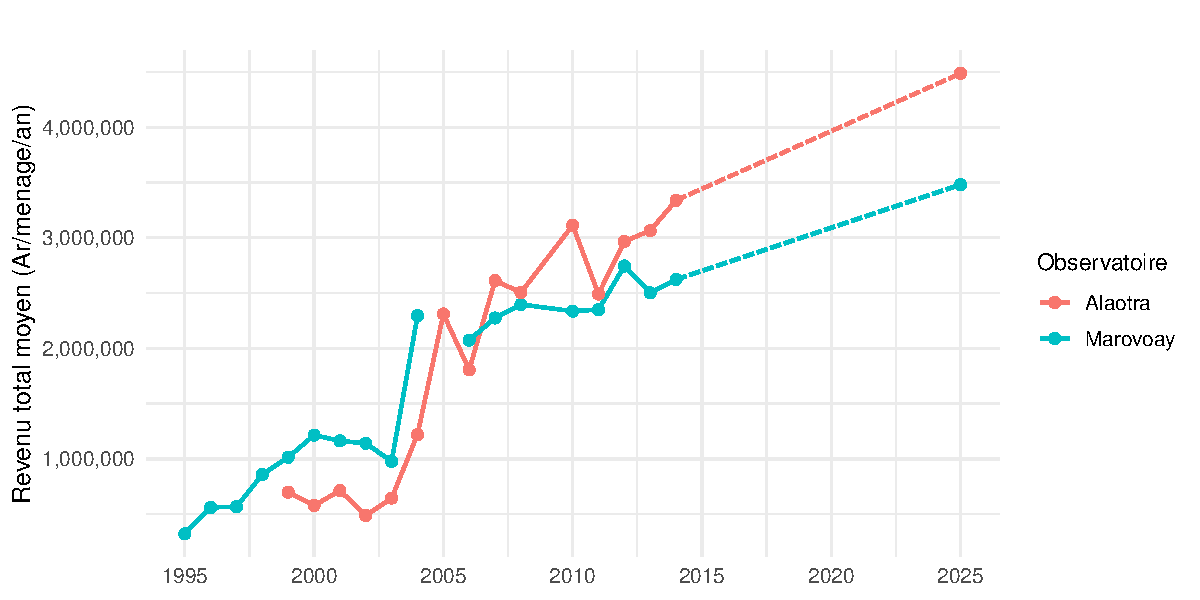
\includegraphics[keepaspectratio]{03_habitat_niveau_de_vie_files/figure-pdf/fig_trends_revtot-1.pdf}}

}

\caption{Evolution du revenu total moyen par menage (Ar courants)}

\end{figure}%

\begin{figure}[H]

{\centering \pandocbounded{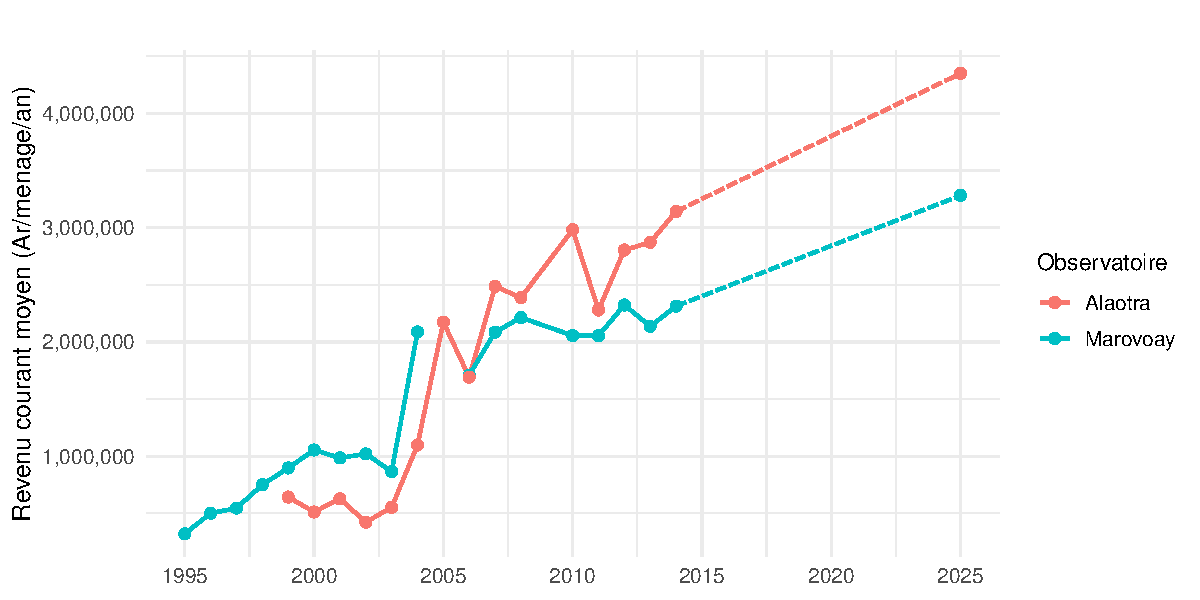
\includegraphics[keepaspectratio]{03_habitat_niveau_de_vie_files/figure-pdf/fig_trends_revcou-1.pdf}}

}

\caption{Evolution du revenu courant moyen par menage (Ar courants)}

\end{figure}%

\begin{figure}[H]

{\centering \pandocbounded{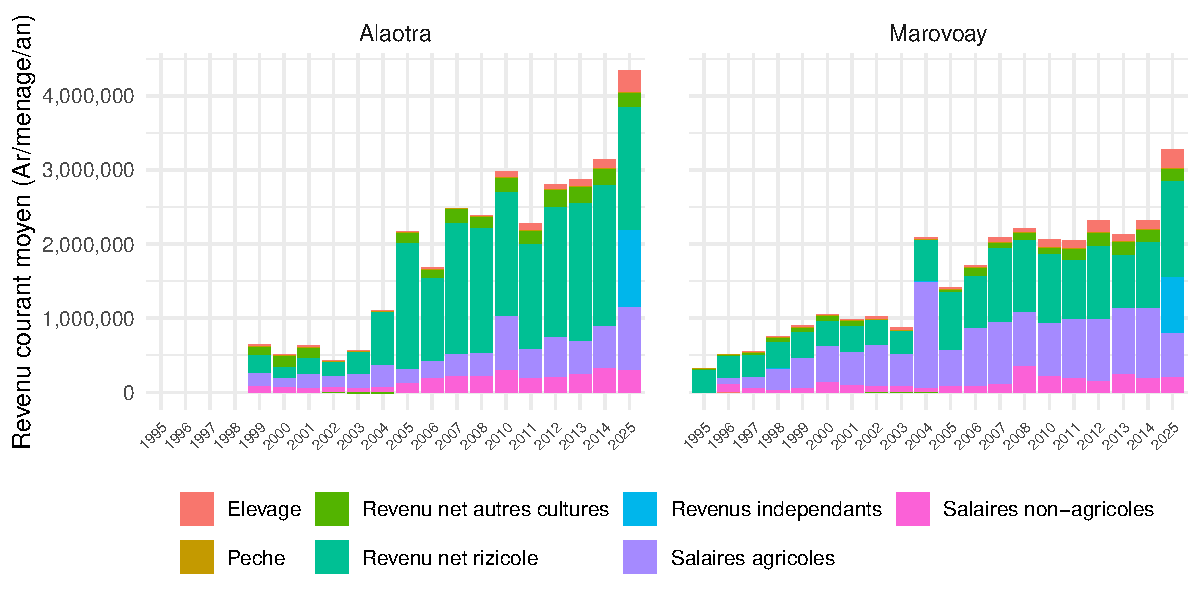
\includegraphics[keepaspectratio]{03_habitat_niveau_de_vie_files/figure-pdf/fig_trends_decomp-1.pdf}}

}

\caption{Evolution des composantes du revenu courant moyen (Ar
courants)}

\end{figure}%

\subsection{Deflation et indices de
prix}\label{deflation-et-indices-de-prix}

La comparaison des revenus sur longue periode necessite de tenir compte
de l'inflation. Nous utilisons ici l'\textbf{IPC national} publie par la
Banque Mondiale (indicateur \texttt{FP.CPI.TOTL}, base 2010 = 100). Cet
indice est calcule a partir d'un panier de consommation urbain ; il ne
reflete donc qu'imparfaitement l'evolution des prix en milieu rural.
Pour 2024-2025, non encore publies par la Banque Mondiale, l'IPC est
extrapole a +9 \% par an.

\begin{tcolorbox}[enhanced jigsaw, colframe=quarto-callout-note-color-frame, colback=white, titlerule=0mm, colbacktitle=quarto-callout-note-color!10!white, toptitle=1mm, opacitybacktitle=0.6, title=\textcolor{quarto-callout-note-color}{\faInfo}\hspace{0.5em}{Note}, left=2mm, leftrule=.75mm, bottomtitle=1mm, coltitle=black, arc=.35mm, rightrule=.15mm, bottomrule=.15mm, toprule=.15mm, opacityback=0, breakable]

Une prochaine version de ce rapport integrera un IPC regional (Boeny
pour Marovoay, Alaotra-Mangoro pour Alaotra), extrait des series de
l'INSTAT ou des enquetes EPM, afin de mieux capter l'inflation locale.

\end{tcolorbox}

\begin{figure}[H]

{\centering \pandocbounded{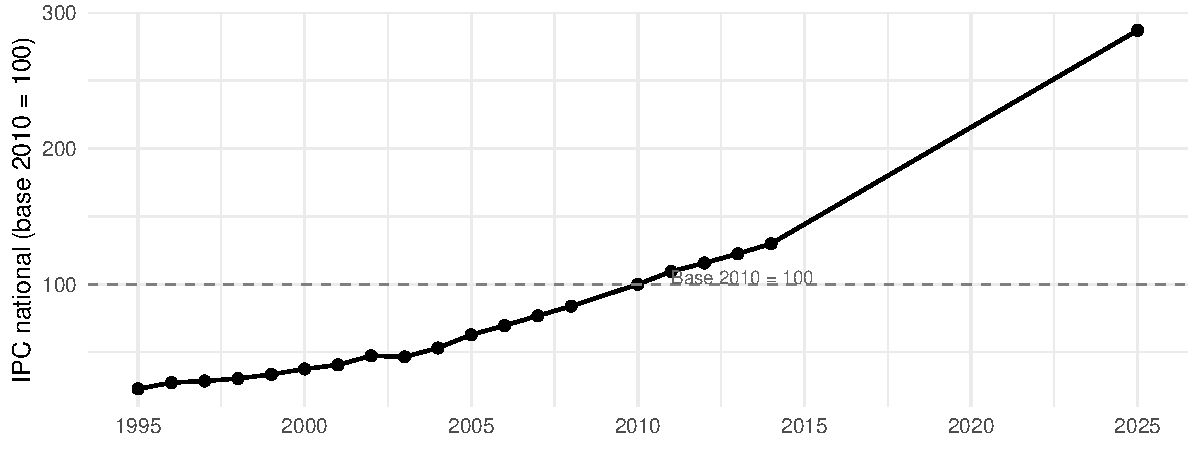
\includegraphics[keepaspectratio]{03_habitat_niveau_de_vie_files/figure-pdf/fig_ipc_national-1.pdf}}

}

\caption{Evolution de l'IPC national Madagascar (base 2010 = 100)}

\end{figure}%

\subsection{Prix median du paddy et comparaison avec
l'IPC}\label{prix-median-du-paddy-et-comparaison-avec-lipc}

Le prix de vente median du paddy, calcule a partir des ventes declarees
par les menages (\texttt{dc24} dans \texttt{res\_dc21}), fournit un
indicateur complementaire de l'inflation locale.

\begin{figure}[H]

{\centering \pandocbounded{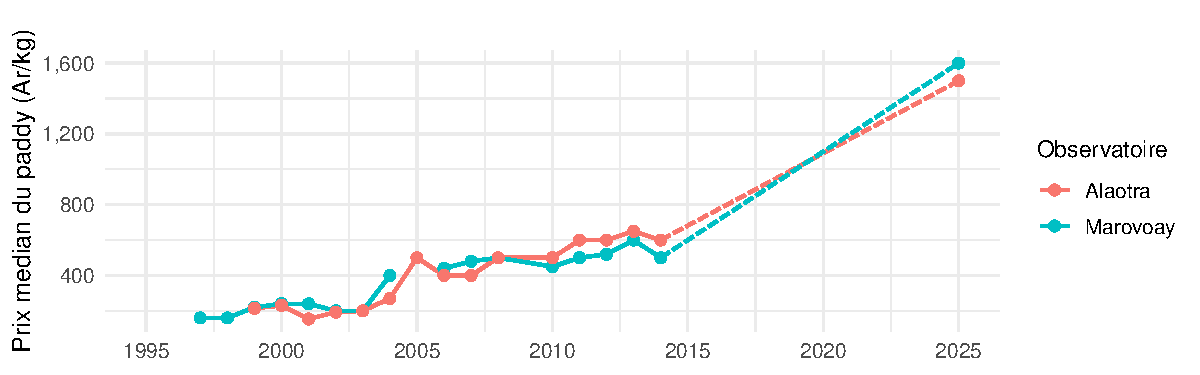
\includegraphics[keepaspectratio]{03_habitat_niveau_de_vie_files/figure-pdf/fig_trends_paddy-1.pdf}}

}

\caption{Evolution du prix median du paddy (Ar/kg)}

\end{figure}%

\begin{figure}[H]

{\centering \pandocbounded{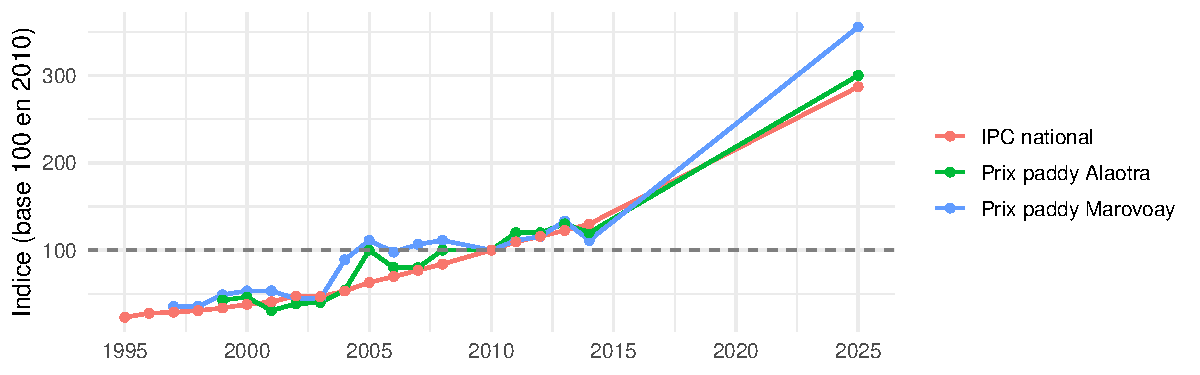
\includegraphics[keepaspectratio]{03_habitat_niveau_de_vie_files/figure-pdf/fig_ipc_vs_paddy-1.pdf}}

}

\caption{Comparaison de l'IPC national et de l'indice du prix du paddy
(base 100 en 2010)}

\end{figure}%

\subsection{Revenus reels (deflates par l'IPC
national)}\label{revenus-reels-deflates-par-lipc-national}

Les revenus nominaux sont convertis en Ariary constants (base 2010) en
divisant par l'IPC national. Ceci permet d'evaluer l'evolution du
pouvoir d'achat, sous reserve des limites du deflateur urbain.

\begin{figure}[H]

{\centering \pandocbounded{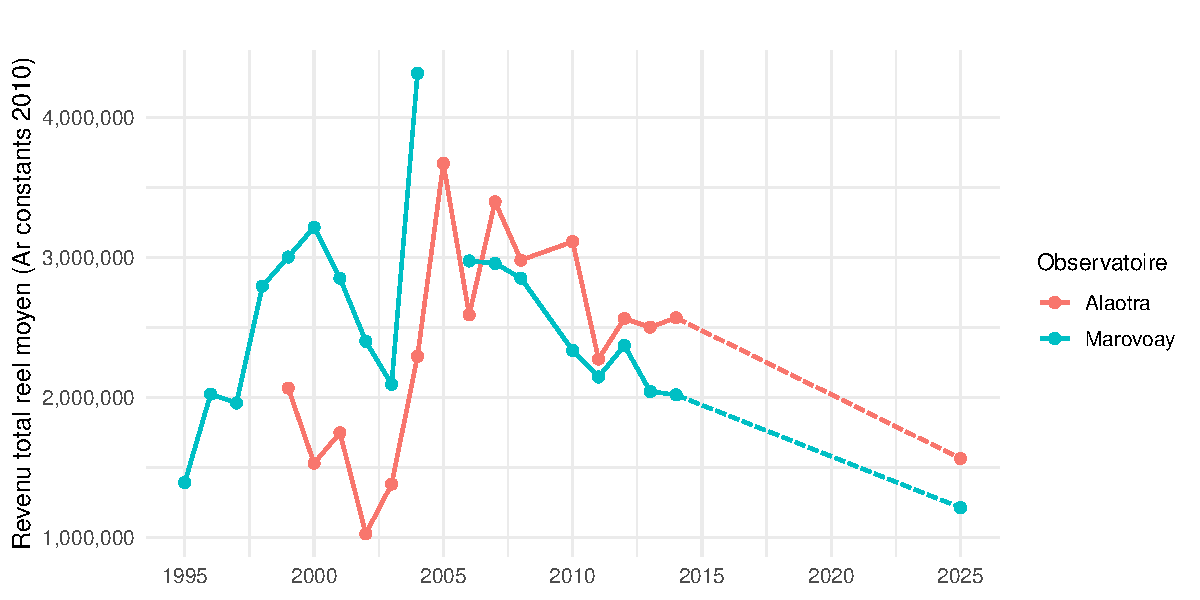
\includegraphics[keepaspectratio]{03_habitat_niveau_de_vie_files/figure-pdf/fig_trends_revtot_real-1.pdf}}

}

\caption{Evolution du revenu total reel moyen par menage (Ar constants
2010, IPC)}

\end{figure}%

\begin{figure}[H]

{\centering \pandocbounded{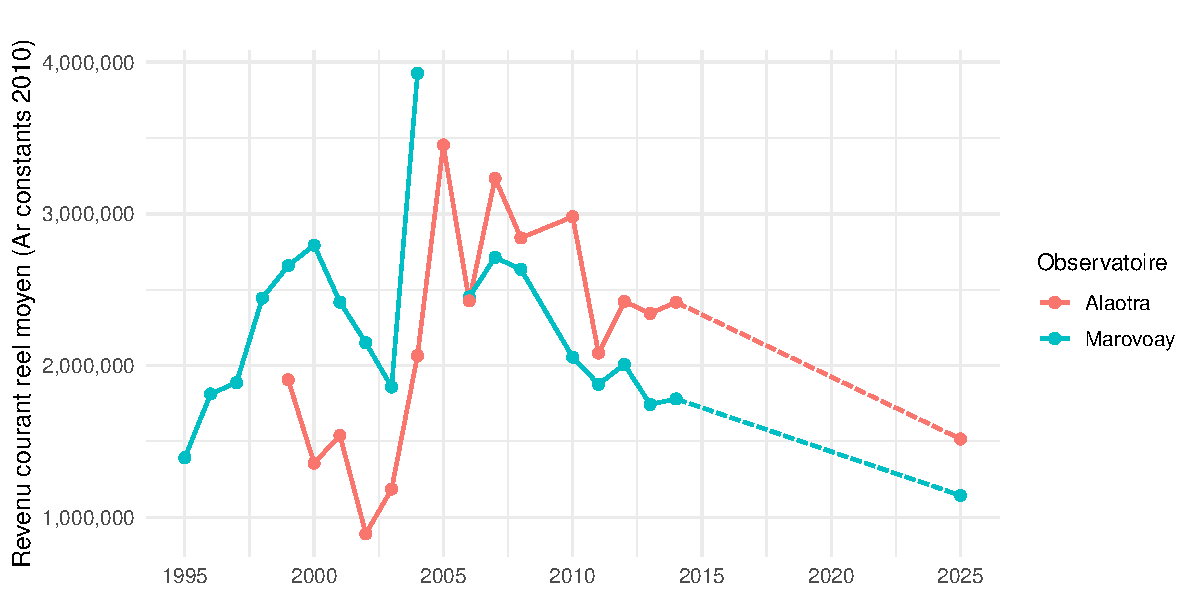
\includegraphics[keepaspectratio]{03_habitat_niveau_de_vie_files/figure-pdf/fig_trends_revcou_real-1.pdf}}

}

\caption{Evolution du revenu courant reel moyen par menage (Ar constants
2010, IPC)}

\end{figure}%

\subsection{Revenus reels (deflates par le prix du
paddy)}\label{revenus-reels-deflates-par-le-prix-du-paddy}

Le prix du paddy, produit central de ces economies rizicoles, offre un
deflateur alternatif plus proche de la realite locale que l'IPC
national. Les revenus sont ici exprimes en equivalent-paddy a prix 2010,
c'est-a-dire divises par l'indice du prix median du paddy de chaque
observatoire (base 2010 = 1). Ce deflateur est propre a chaque
observatoire.

\begin{figure}[H]

{\centering \pandocbounded{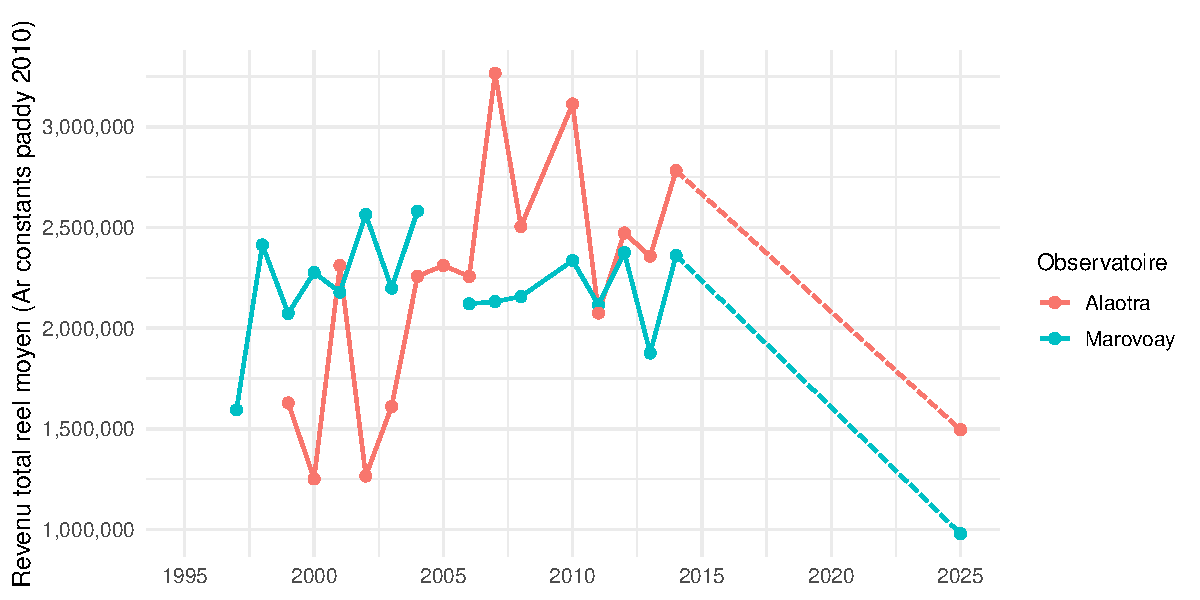
\includegraphics[keepaspectratio]{03_habitat_niveau_de_vie_files/figure-pdf/fig_trends_revtot_paddy-1.pdf}}

}

\caption{Evolution du revenu total reel moyen par menage (Ar constants
paddy 2010)}

\end{figure}%

\begin{figure}[H]

{\centering \pandocbounded{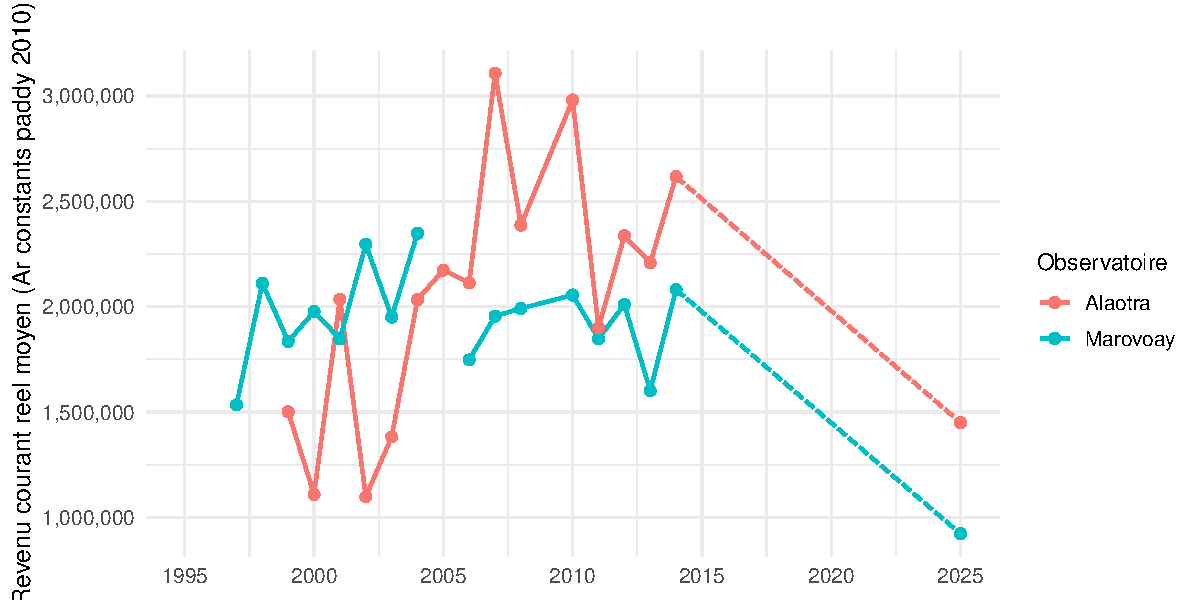
\includegraphics[keepaspectratio]{03_habitat_niveau_de_vie_files/figure-pdf/fig_trends_revcou_paddy-1.pdf}}

}

\caption{Evolution du revenu courant reel moyen par menage (Ar constants
paddy 2010)}

\end{figure}%

\section{Evolution des conditions d'habitat
(1997-2025)}\label{sec-habitat-multiyear}

Les donnees sur l'habitat permettent de suivre l'evolution de la source
d'eclairage (acces a l'electricite) et de la source d'eau principale sur
la periode couverte.

\begin{figure}[H]

{\centering \pandocbounded{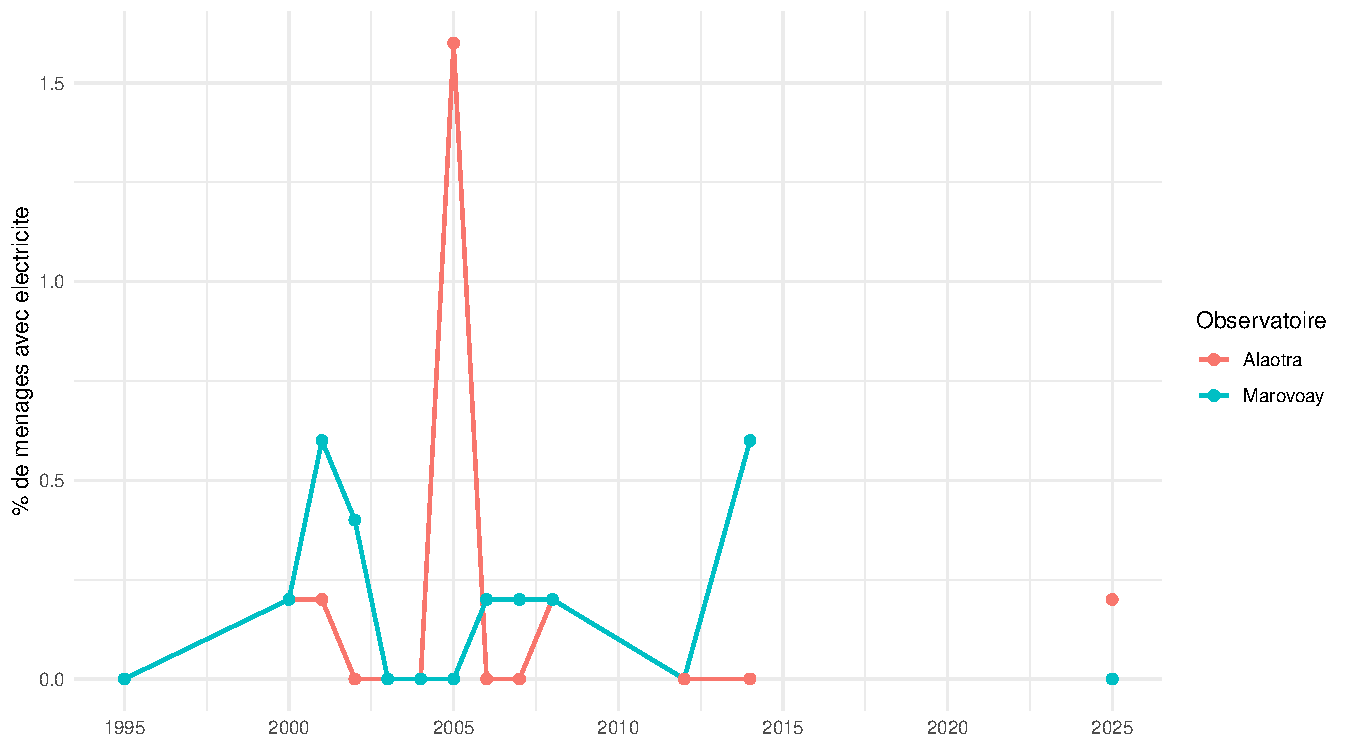
\includegraphics[keepaspectratio]{03_habitat_niveau_de_vie_files/figure-pdf/fig_habitat_elec-1.pdf}}

}

\caption{Evolution de l'acces a l'electricite (1997-2025)}

\end{figure}%

\begin{figure}[H]

{\centering \pandocbounded{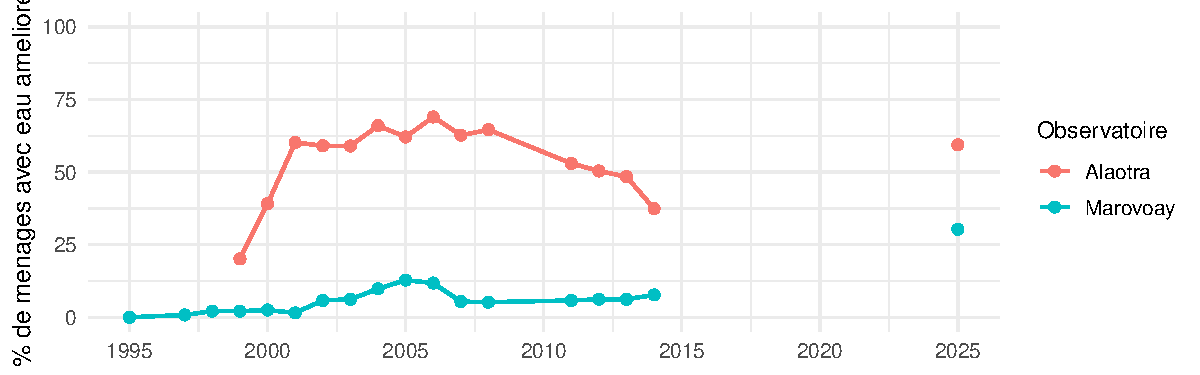
\includegraphics[keepaspectratio]{03_habitat_niveau_de_vie_files/figure-pdf/fig_habitat_water-1.pdf}}

}

\caption{Evolution de l'acces a une source d'eau amelioree (1997-2025)}

\end{figure}%

\bookmarksetup{startatroot}

\chapter{Foncier}\label{foncier}

Ce chapitre analyse la situation foncière des ménages des observatoires
d'Alaotra et de Marovoay : patrimoine foncier possédé, parcelles
exploitées sans en être propriétaire, cessions à des tiers, sécurisation
foncière, et satisfaction des ménages par rapport à leur dotation en
terre.

\begin{tcolorbox}[enhanced jigsaw, colframe=quarto-callout-warning-color-frame, colback=white, titlerule=0mm, colbacktitle=quarto-callout-warning-color!10!white, toptitle=1mm, opacitybacktitle=0.6, title=\textcolor{quarto-callout-warning-color}{\faExclamationTriangle}\hspace{0.5em}{Travail de vérification en cours}, left=2mm, leftrule=.75mm, bottomtitle=1mm, coltitle=black, arc=.35mm, rightrule=.15mm, bottomrule=.15mm, toprule=.15mm, opacityback=0, breakable]

Les résultats présentés ci-dessous sont provisoires, et sont
susceptibles de faire l'objet de corrections.

\end{tcolorbox}

\section{Patrimoine foncier}\label{sec-patrimoine}

\subsection{Nombre de parcelles
possédées}\label{nombre-de-parcelles-possuxe9duxe9es}

Sur les 1026 ménages enquêtés, 490 (47.8 \%) ne possèdent aucune
parcelle. La très grande majorité des ménages (52.2 \%) sont donc
propriétaires d'au moins une parcelle (Figure~\ref{fig-nb-parcelles}).
Les ménages propriétaires possèdent en moyenne 2.2 parcelles.

\textbf{Alaotra.} Les ménages propriétaires possèdent en moyenne 2.3
parcelles.

\textbf{Marovoay.} Les ménages propriétaires possèdent en moyenne 2
parcelles.

\begin{figure}

\centering{

\pandocbounded{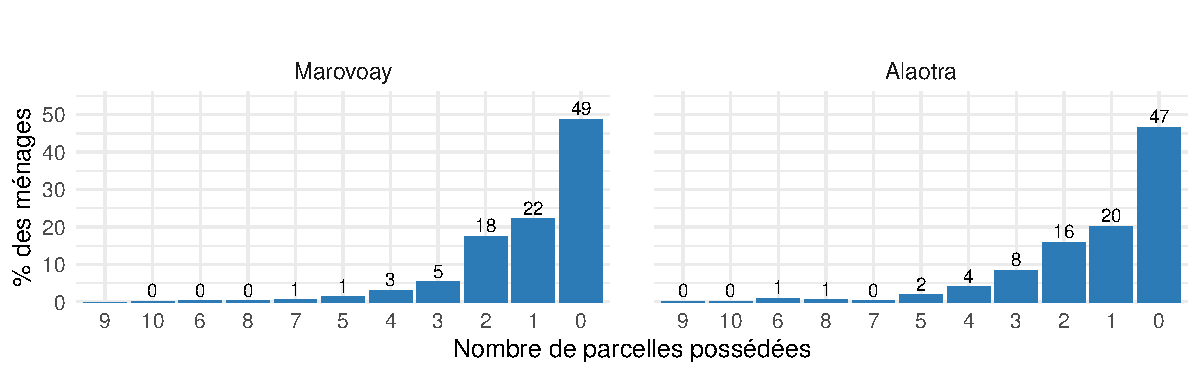
\includegraphics[keepaspectratio]{04_foncier_files/figure-pdf/fig-nb-parcelles-1.pdf}}

}

\caption{\label{fig-nb-parcelles}Distribution du nombre de parcelles
possédées par ménage}

\end{figure}%

\begin{table}

\caption{\label{tbl-parcelles-stats}Statistiques sur le patrimoine
foncier possédé}

\centering{

\caption*{
{\fontsize{20}{25}\selectfont  Patrimoine foncier des ménages propriétaires\fontsize{12}{15}\selectfont }
} 
\fontsize{12.0pt}{14.0pt}\selectfont
\begin{tabular*}{\linewidth}{@{\extracolsep{\fill}}llrr}
\toprule
Indicateur & Stat & Alaotra & Marovoay \\ 
\midrule\addlinespace[2.5pt]
Nb parcelles / ménage & Moyenne & 2.3 & 2.1 \\ 
Nb parcelles / ménage & Mediane & 2.0 & 2.0 \\ 
Superficie / parcelle (ares) & Moyenne & 51.6 & 78.9 \\ 
Superficie / parcelle (ares) & Mediane & 20.0 & 50.0 \\ 
Superficie totale / ménage (ares) & Moyenne & 117.4 & 163.2 \\ 
Superficie totale / ménage (ares) & Mediane & 50.0 & 100.0 \\ 
\bottomrule
\end{tabular*}

}

\end{table}%

Le Table~\ref{tbl-parcelles-stats} résume les principales
caractéristiques du patrimoine foncier possédé.

\textbf{Alaotra.} La superficie moyenne par parcelle est de 51.6 ares,
et la surface totale possédée par ménage atteint en moyenne 117.4 ares.

\textbf{Marovoay.} La superficie moyenne par parcelle est de 78.9 ares,
et la surface totale possédée par ménage atteint en moyenne 163.2 ares.

\subsection{Type et localisation des parcelles
possédées}\label{type-et-localisation-des-parcelles-possuxe9duxe9es}

Le patrimoine foncier des ménages se compose principalement de rizières
et de champs de cultures pluviales (Figure~\ref{fig-type-parcelle}).

\textbf{Alaotra.} Les rizières représentent 52.3 \% des parcelles
possédées et les champs 40.4 \%.

\textbf{Marovoay.} Les rizières représentent 73.9 \% des parcelles
possédées et les champs 25.6 \%.

\begin{figure}

\centering{

\pandocbounded{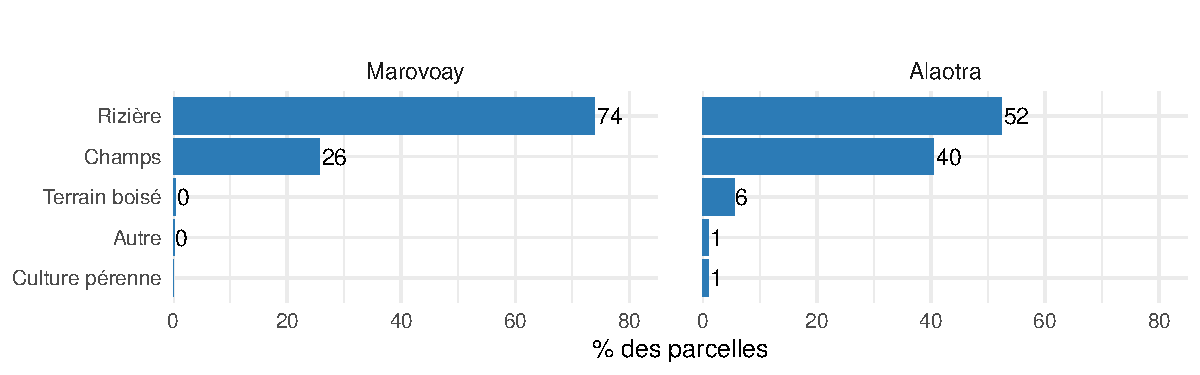
\includegraphics[keepaspectratio]{04_foncier_files/figure-pdf/fig-type-parcelle-1.pdf}}

}

\caption{\label{fig-type-parcelle}Type des parcelles possédées}

\end{figure}%

La localisation des parcelles reflète les spécificités agro-écologiques
de chaque site (Figure~\ref{fig-localisation-parcelle}).

\textbf{Alaotra.} Les parcelles se concentrent principalement en plaine
(45.3 \%).

\textbf{Marovoay.} La localisation la plus fréquente est la plaine (67.3
\%).

\begin{figure}

\centering{

\pandocbounded{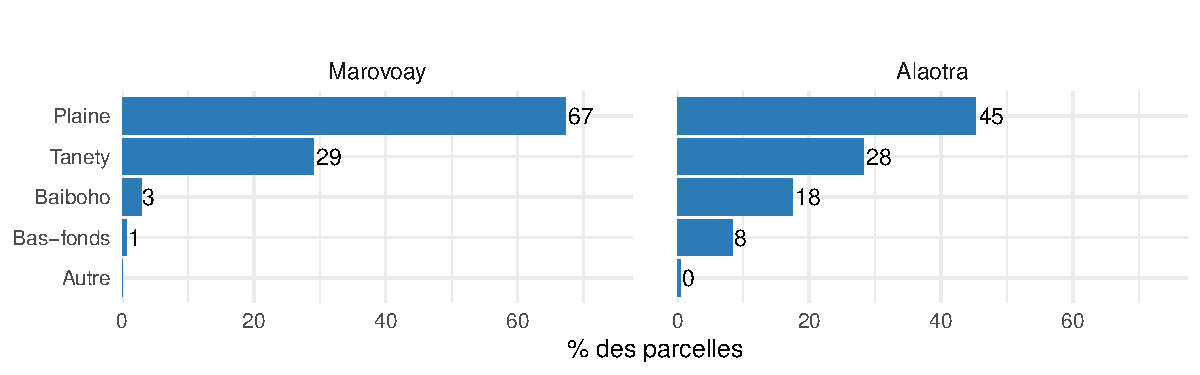
\includegraphics[keepaspectratio]{04_foncier_files/figure-pdf/fig-localisation-parcelle-1.pdf}}

}

\caption{\label{fig-localisation-parcelle}Localisation des parcelles
possédées}

\end{figure}%

\subsection{Irrigation des parcelles
possédées}\label{irrigation-des-parcelles-possuxe9duxe9es}

L'accès à l'irrigation est un facteur déterminant de la productivité
rizicole. La Figure~\ref{fig-irrigation-possedee} présente les modes
d'irrigation des parcelles possédées par les ménages dans les deux
observatoires. Les différences entre Alaotra et Marovoay reflètent les
investissements hydrauliques historiques de chaque périmètre.

\begin{figure}

\centering{

\pandocbounded{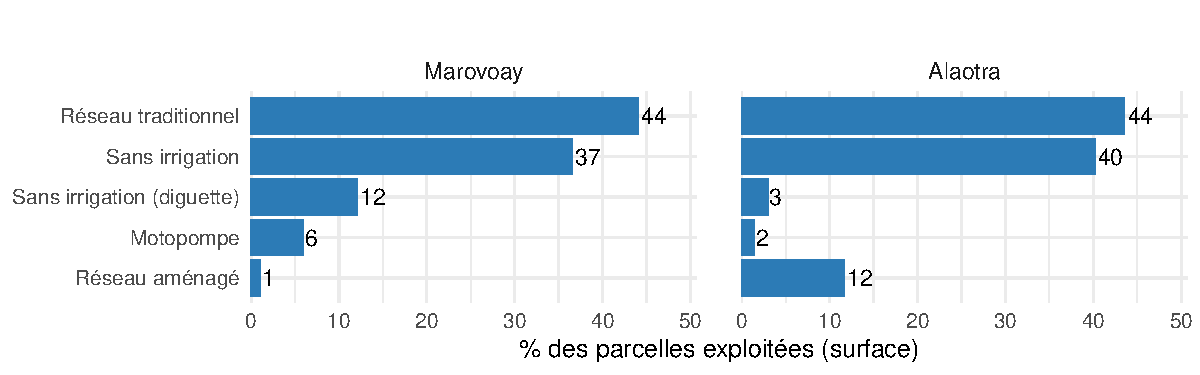
\includegraphics[keepaspectratio]{04_foncier_files/figure-pdf/fig-irrigation-possedee-1.pdf}}

}

\caption{\label{fig-irrigation-possedee}Mode d'irrigation des parcelles
possédées}

\end{figure}%

\subsection{Mode d'acquisition et
ancienneté}\label{mode-dacquisition-et-anciennetuxe9}

Le mode d'acquisition des parcelles renseigne sur la dynamique du marché
foncier et le poids des transmissions familiales
(Figure~\ref{fig-acquisition}). L'héritage domine largement dans les
deux observatoires.

\textbf{Alaotra.} L'héritage concerne 46.5 \% des parcelles, l'achat
49.1 \% et la mise en valeur 1.1 \%.

\textbf{Marovoay.} L'héritage concerne 59.4 \% des parcelles, l'achat 39
\% et la mise en valeur 0.2 \%.

\begin{figure}

\centering{

\pandocbounded{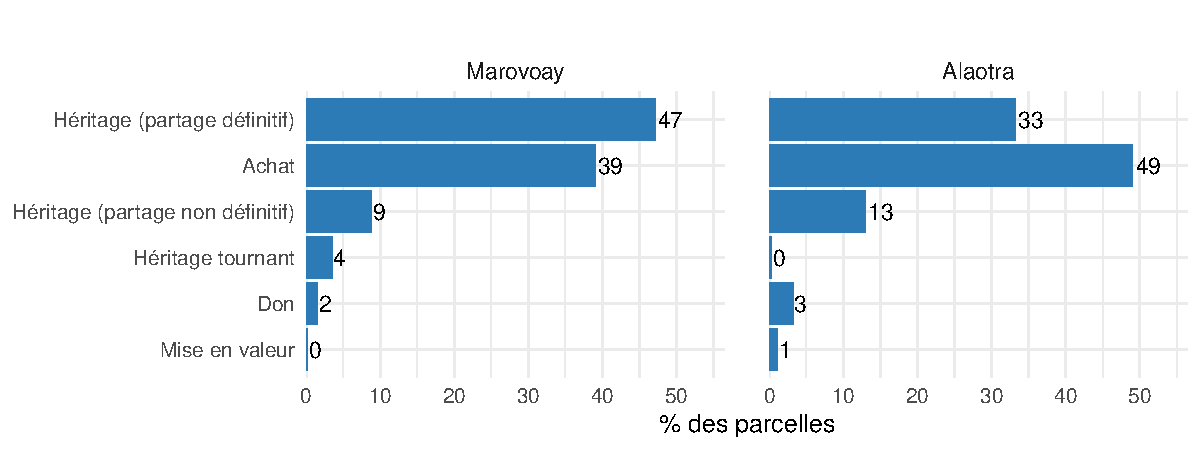
\includegraphics[keepaspectratio]{04_foncier_files/figure-pdf/fig-acquisition-1.pdf}}

}

\caption{\label{fig-acquisition}Mode d'acquisition des parcelles
possédées}

\end{figure}%

L'ancienneté de possession témoigne de l'enracinement des ménages sur
leurs terres (Figure~\ref{fig-anciennete}). Une part importante des
parcelles est détenue depuis plusieurs décennies, reflétant la
continuité de l'occupation foncière dans les deux zones. Les
acquisitions récentes (années 2010 et au-delà) sont toutefois
observables, signe que le marché foncier reste actif.

\begin{figure}

\centering{

\pandocbounded{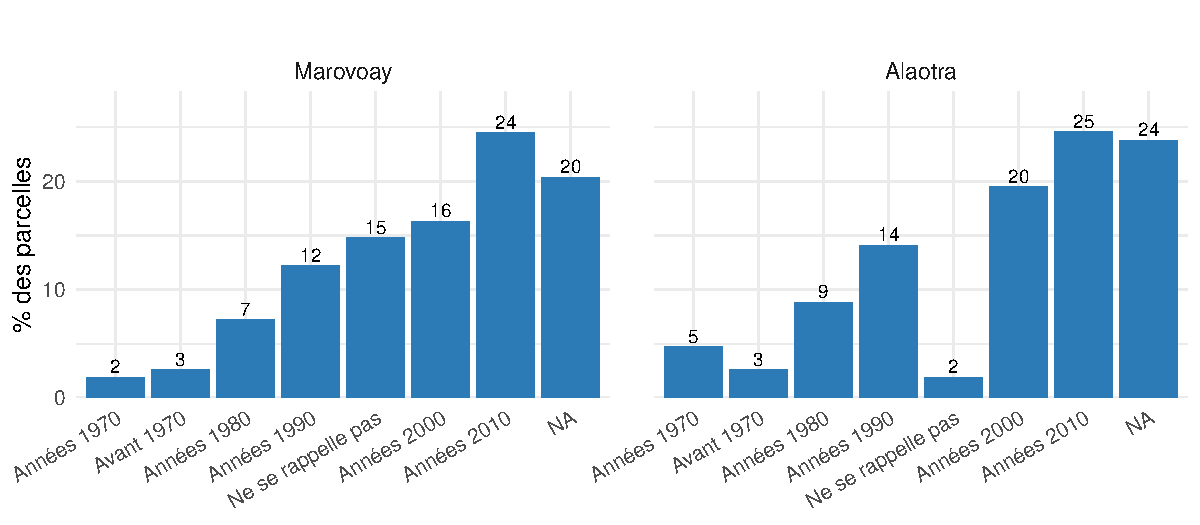
\includegraphics[keepaspectratio]{04_foncier_files/figure-pdf/fig-anciennete-1.pdf}}

}

\caption{\label{fig-anciennete}Ancienneté de possession des parcelles}

\end{figure}%

\subsection{Propriétaire dans le
ménage}\label{propriuxe9taire-dans-le-muxe9nage}

La question de l'identité du propriétaire au sein du ménage soulève des
enjeux de genre importants (Figure~\ref{fig-proprietaire}). Dans les
deux observatoires, c'est le chef de ménage qui est déclaré propriétaire
de la majorité des parcelles, ce qui illustre les inégalités d'accès au
foncier.

\textbf{Alaotra.} Le chef de ménage est propriétaire de 63.5 \% des
parcelles ; le ou la conjoint(e) n'apparaît que dans 15.6 \% des cas.

\textbf{Marovoay.} Le chef de ménage est propriétaire de 76.3 \% des
parcelles ; le ou la conjoint(e) n'apparaît que dans 8.8 \% des cas.

\begin{figure}

\centering{

\pandocbounded{
\includegraphics[keepaspectratio]{04_foncier_files/figure-pdf/fig-proprietaire-1.pdf}}

}

\caption{\label{fig-proprietaire}Qui dans le ménage est propriétaire de
la parcelle}

\end{figure}%

\section{Sécurisation foncière}\label{sec-securisation}

La sécurisation foncière est un enjeu majeur à Madagascar. Les ménages
peuvent détenir un titre foncier, un certificat foncier (délivré par le
guichet foncier communal), ou divers documents informels. Les résultats
de l'enquête révèlent un niveau de sécurisation formelle encore très
faible (Table~\ref{tbl-securisation}).

\textbf{Alaotra.} Seules 16.2 \% des parcelles disposent d'un titre
foncier. Les certificats fonciers ne couvrent que 27.5 \% des parcelles.

\textbf{Marovoay.} Seules 21.5 \% des parcelles disposent d'un titre
foncier. Les certificats fonciers ne couvrent que 28.3 \% des parcelles.

\begin{table}

\caption{\label{tbl-securisation}Sécurisation foncière des parcelles
possédées}

\centering{

\caption*{
{\fontsize{20}{25}\selectfont  \% des parcelles disposant d'un document de sécurisation\fontsize{12}{15}\selectfont }
} 
\fontsize{12.0pt}{14.0pt}\selectfont
\begin{tabular*}{\linewidth}{@{\extracolsep{\fill}}lrr}
\toprule
Document & Alaotra (\%) & Marovoay (\%) \\ 
\midrule\addlinespace[2.5pt]
Titre foncier & 16.2 & 21.5 \\ 
Certificat foncier & 27.5 & 28.3 \\ 
\bottomrule
\end{tabular*}

}

\end{table}%

En l'absence de titre ou de certificat, les ménages s'appuient sur des
documents informels de nature très variable (Figure~\ref{fig-papiers}).
Cependant, 34.5 \% des parcelles ne sont accompagnées d'aucun document
justificatif, ce qui expose ces ménages à un risque élevé d'insécurité
foncière en cas de litige.

\begin{figure}

\centering{

\pandocbounded{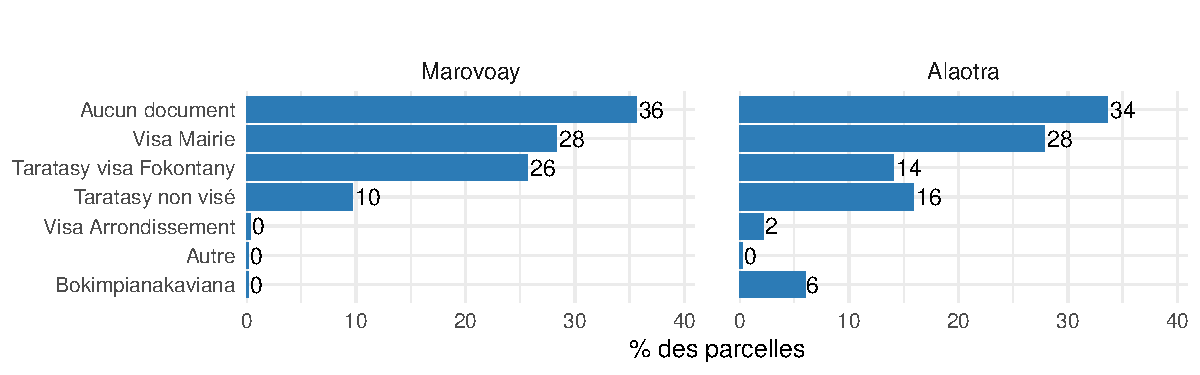
\includegraphics[keepaspectratio]{04_foncier_files/figure-pdf/fig-papiers-1.pdf}}

}

\caption{\label{fig-papiers}Autres documents prouvant la possession}

\end{figure}%

\section{Parcelles cédées à des tiers}\label{sec-cessions}

Les ménages propriétaires peuvent céder certaines de leurs parcelles à
d'autres exploitants, sous forme de prêt, location, métayage ou mise en
gage (Table~\ref{tbl-cession-pratique}), pour un total de 132 parcelles
cédées.

\textbf{Alaotra.} Cette pratique concerne 9.3 \% des ménages.

\textbf{Marovoay.} Cette pratique concerne 10.6 \% des ménages.

\begin{table}

\caption{\label{tbl-cession-pratique}Ménages cédant des parcelles à des
tiers}

\centering{

\caption*{
{\fontsize{20}{25}\selectfont  Ménages cédant des parcelles à des tiers\fontsize{12}{15}\selectfont }
} 
\fontsize{12.0pt}{14.0pt}\selectfont
\begin{tabular*}{\linewidth}{@{\extracolsep{\fill}}lrrr}
\toprule
Observatory & Nb ménages & Cèdent (nb) & Cèdent (\%) \\ 
\midrule\addlinespace[2.5pt]
Alaotra & 507 & 47 & 9.3 \\ 
Marovoay & 518 & 55 & 10.6 \\ 
\bottomrule
\end{tabular*}

}

\end{table}%

Parmi les parcelles cédées, les modes de faire-valoir varient
sensiblement d'un observatoire à l'autre
(Figure~\ref{fig-mode-cession}). Le prêt et le métayage sont les formes
les plus courantes de cession, le métayage occupant une place
particulièrement importante dans les zones rizicoles.

\begin{figure}

\centering{

\pandocbounded{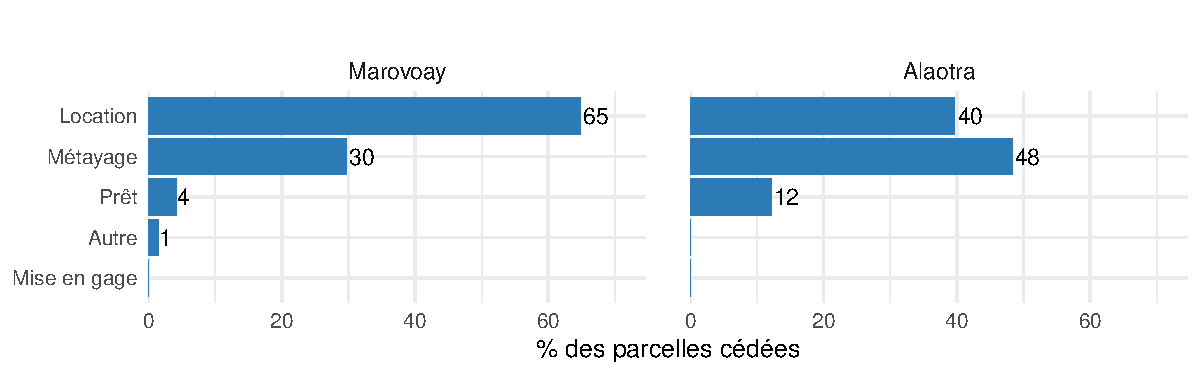
\includegraphics[keepaspectratio]{04_foncier_files/figure-pdf/fig-mode-cession-1.pdf}}

}

\caption{\label{fig-mode-cession}Mode de faire-valoir des parcelles
cédées}

\end{figure}%

Les motivations de la cession reflètent des stratégies économiques
diversifiées (Figure~\ref{fig-motif-cession}). Pour certains ménages,
céder une parcelle répond à un besoin de liquidités ou à l'impossibilité
de cultiver l'ensemble de leur patrimoine ; pour d'autres, il s'agit de
maintenir un lien social avec la parenté ou le voisinage.

\begin{figure}

\centering{

\pandocbounded{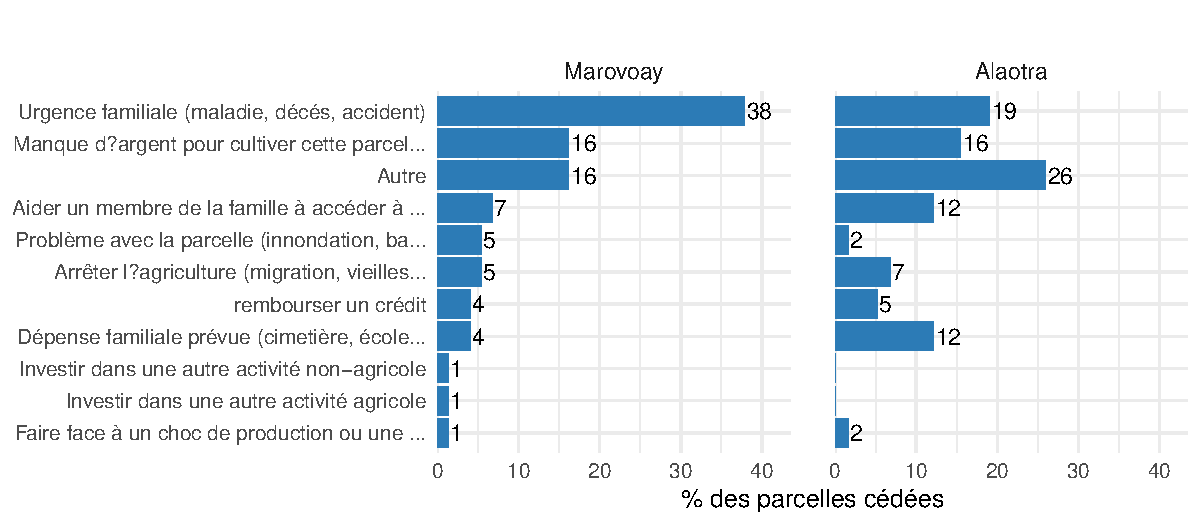
\includegraphics[keepaspectratio]{04_foncier_files/figure-pdf/fig-motif-cession-1.pdf}}

}

\caption{\label{fig-motif-cession}Motif de la cession de parcelles}

\end{figure}%

Les bénéficiaires des cessions sont principalement des membres de la
famille ou des voisins (Figure~\ref{fig-cedee-a-qui}), ce qui confirme
le caractère en grande partie familial et communautaire du marché
foncier local.

\begin{figure}

\centering{

\pandocbounded{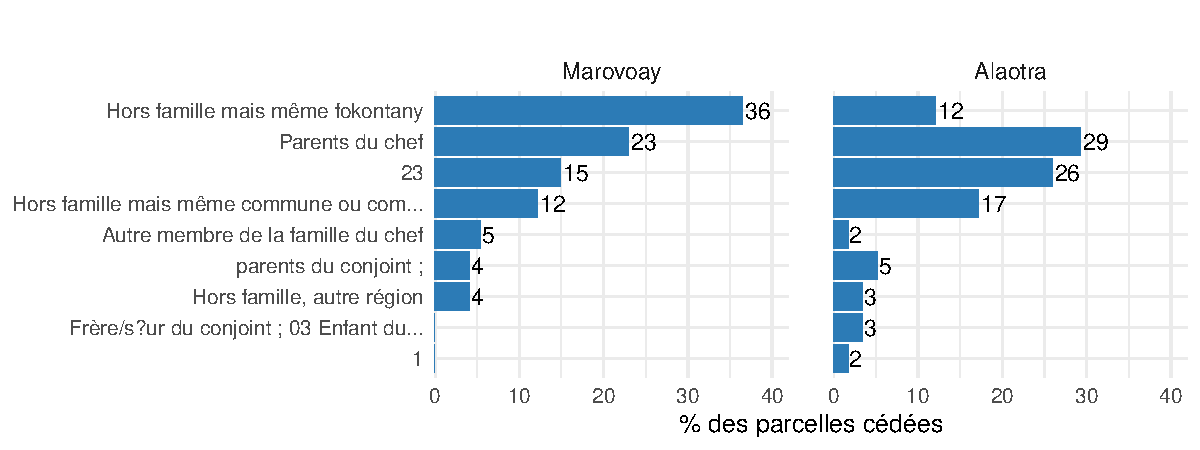
\includegraphics[keepaspectratio]{04_foncier_files/figure-pdf/fig-cedee-a-qui-1.pdf}}

}

\caption{\label{fig-cedee-a-qui}À qui la parcelle est-elle cédée}

\end{figure}%

\section{Parcelles exploitées non possédées}\label{sec-exploitees}

En plus de leurs propres parcelles, de nombreux ménages exploitent des
terres appartenant à d'autres propriétaires
(Table~\ref{tbl-exploitation-autres}), pour un total de 713 parcelles.
Le recours à l'exploitation de terres d'autrui traduit soit une
insuffisance du patrimoine propre, soit une stratégie de diversification
de l'assiette foncière cultivée.

\textbf{Alaotra.} Cette pratique concerne 45.6 \% des ménages.

\textbf{Marovoay.} Cette pratique concerne 46.8 \% des ménages.

\begin{table}

\caption{\label{tbl-exploitation-autres}Ménages exploitant des parcelles
non possédées}

\centering{

\caption*{
{\fontsize{20}{25}\selectfont  Ménages exploitant des parcelles d'autrui\fontsize{12}{15}\selectfont }
} 
\fontsize{12.0pt}{14.0pt}\selectfont
\begin{tabular*}{\linewidth}{@{\extracolsep{\fill}}lrrr}
\toprule
Observatory & Nb ménages & Exploitent (nb) & Exploitent (\%) \\ 
\midrule\addlinespace[2.5pt]
Alaotra & 507 & 231 & 45.6 \\ 
Marovoay & 519 & 243 & 46.8 \\ 
\bottomrule
\end{tabular*}

}

\end{table}%

Les parcelles exploitées sans en être propriétaire sont, comme les
parcelles possédées, majoritairement des rizières
(Figure~\ref{fig-type-exploitee}), reflétant la place centrale de la
riziculture dans les stratégies des ménages.

\begin{figure}

\centering{

\pandocbounded{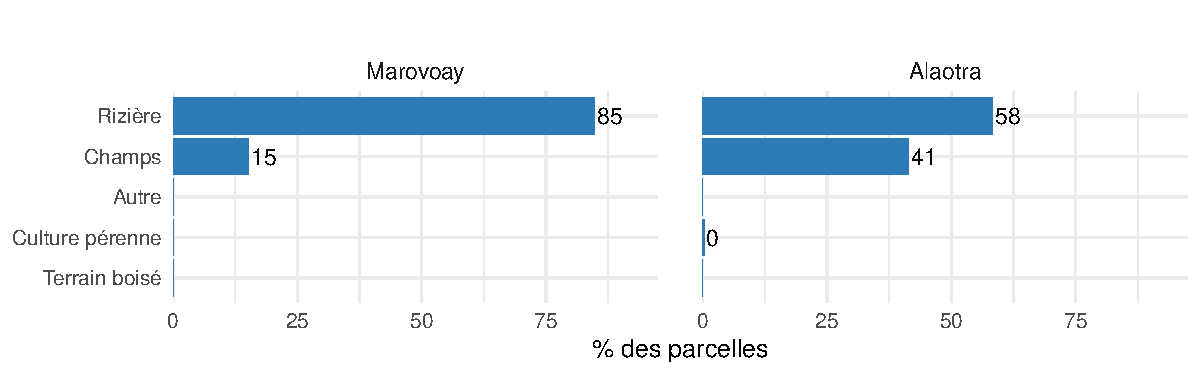
\includegraphics[keepaspectratio]{04_foncier_files/figure-pdf/fig-type-exploitee-1.pdf}}

}

\caption{\label{fig-type-exploitee}Type des parcelles exploitées (non
possédées)}

\end{figure}%

Le mode de faire-valoir des parcelles exploitées révèle l'équilibre
local entre prêt, location et métayage (Figure~\ref{fig-fv-exploitee}).
Le métayage, qui consiste à partager la récolte avec le propriétaire,
reste une forme d'accès au foncier particulièrement répandue.

\begin{figure}

\centering{

\pandocbounded{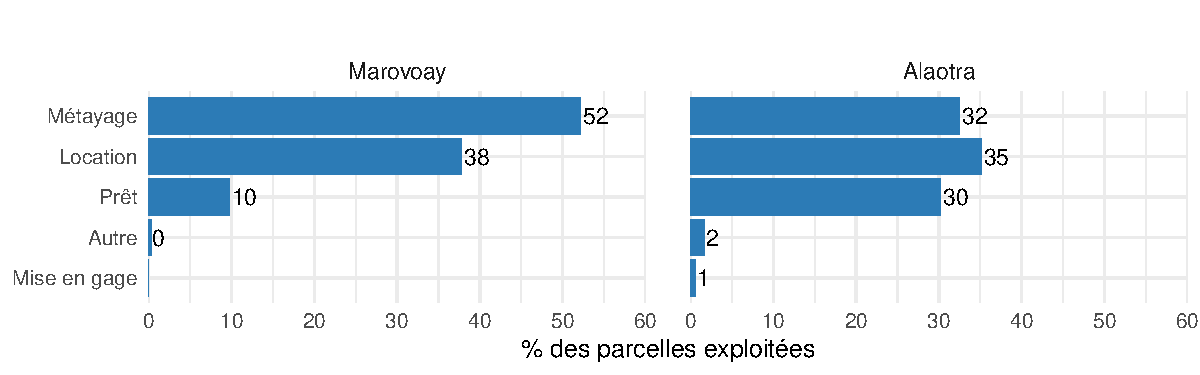
\includegraphics[keepaspectratio]{04_foncier_files/figure-pdf/fig-fv-exploitee-1.pdf}}

}

\caption{\label{fig-fv-exploitee}Mode de faire-valoir des parcelles
exploitées}

\end{figure}%

Les parcelles exploitées appartiennent le plus souvent à des membres de
la famille ou à des voisins (Figure~\ref{fig-proprietaire-exploitee}),
ce qui témoigne du rôle des réseaux de proximité dans l'accès au
foncier.

\begin{figure}

\centering{

\pandocbounded{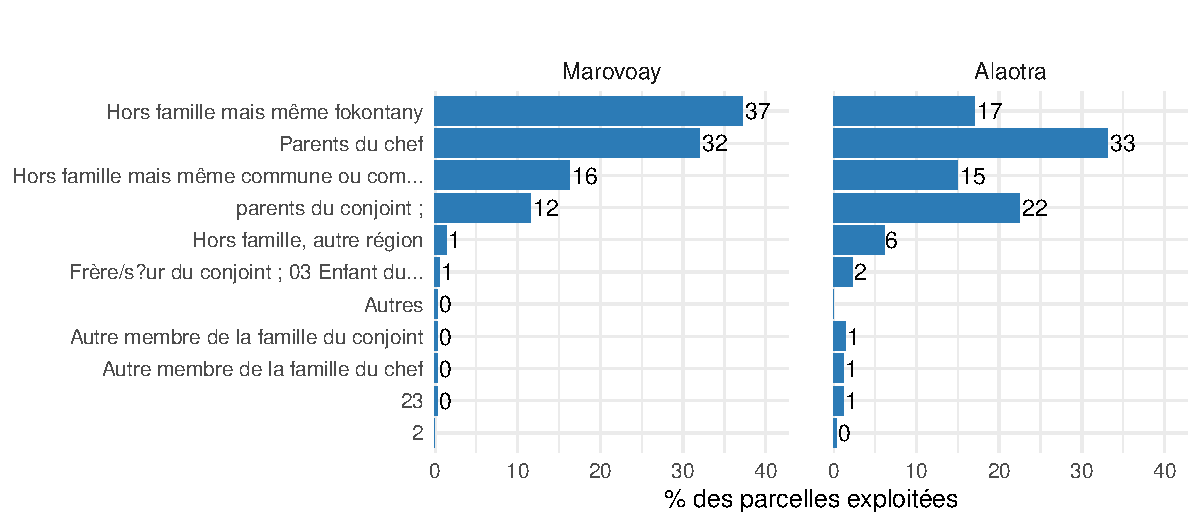
\includegraphics[keepaspectratio]{04_foncier_files/figure-pdf/fig-proprietaire-exploitee-1.pdf}}

}

\caption{\label{fig-proprietaire-exploitee}Propriétaire des parcelles
exploitées}

\end{figure}%

Le mode d'irrigation des parcelles exploitées diffère-t-il de celui des
parcelles possédées ? La Figure~\ref{fig-irrigation-exploitee} permet
d'examiner si les ménages qui exploitent des terres d'autrui accèdent à
des parcelles de même qualité irriguée.

\begin{figure}

\centering{

\pandocbounded{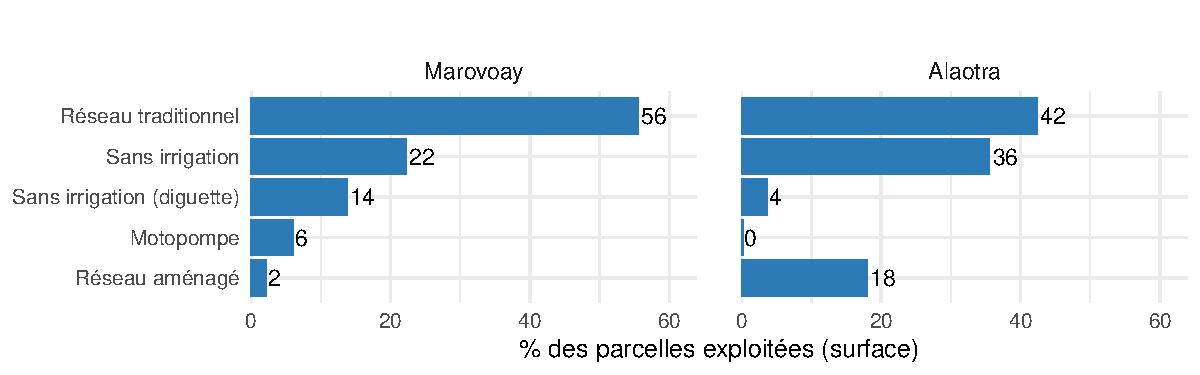
\includegraphics[keepaspectratio]{04_foncier_files/figure-pdf/fig-irrigation-exploitee-1.pdf}}

}

\caption{\label{fig-irrigation-exploitee}Mode d'irrigation des parcelles
exploitées}

\end{figure}%

Le coût de l'exploitation de terres d'autrui varie selon le mode de
faire-valoir (Table~\ref{tbl-rente-exploitee}). Les ménages locataires
versent une rente en argent ou en nature, tandis que les métayers cèdent
une part de la récolte au propriétaire, généralement comprise entre un
quart et la moitié de la production.

\begin{table}

\caption{\label{tbl-rente-exploitee}Rentes versées pour les parcelles
exploitées}

\centering{

\caption*{
{\fontsize{20}{25}\selectfont  Conditions des parcelles exploitées par mode de faire-valoir\fontsize{12}{15}\selectfont }
} 
\fontsize{12.0pt}{14.0pt}\selectfont
\begin{tabular*}{\linewidth}{@{\extracolsep{\fill}}lcrrrr}
\toprule
Observatory & Mode & Nb parcelles & Rente argent moy. (Ar) & Rente produit moy. (kg) & \% métayage moyen \\ 
\midrule\addlinespace[2.5pt]
Alaotra & Location & 122 & 211 & 813 & 22.2 \\ 
Alaotra & Métayage & 113 & 0 & 527 & 48.8 \\ 
Alaotra & Prêt & 105 & 0 & 7 & 6.5 \\ 
Alaotra & Autre & 6 & 100 & 250 & 35.0 \\ 
Alaotra & Mise en gage & 2 & 150 & NaN & 75.0 \\ 
Marovoay & Métayage & 189 & 1 & 264 & 49.4 \\ 
Marovoay & Location & 137 & 202 & 0 & 0.0 \\ 
Marovoay & Prêt & 35 & 19 & 0 & 0.0 \\ 
Marovoay & Autre & 1 & 0 & 240 & 50.0 \\ 
\bottomrule
\end{tabular*}

}

\end{table}%

\section{Abandon de parcelles}\label{sec-abandon}

L'abandon de la culture de certaines parcelles peut révéler des
difficultés structurelles (dégradation des sols, problèmes d'irrigation,
insécurité) ou conjoncturelles (manque de main-d'œuvre, coût des
intrants) (Table~\ref{tbl-abandon}).

\textbf{Alaotra.} Cette pratique touche 18.9 \% des ménages.

\textbf{Marovoay.} Cette pratique touche 16.8 \% des ménages.

\begin{table}

\caption{\label{tbl-abandon}Ménages ayant abandonné la culture de
parcelles}

\centering{

\caption*{
{\fontsize{20}{25}\selectfont  Abandon de la culture d'une ou plusieurs parcelles\fontsize{12}{15}\selectfont }
} 
\fontsize{12.0pt}{14.0pt}\selectfont
\begin{tabular*}{\linewidth}{@{\extracolsep{\fill}}lrrr}
\toprule
Observatory & Nb ménages & Ont abandonné (nb) & Ont abandonné (\%) \\ 
\midrule\addlinespace[2.5pt]
Alaotra & 281 & 53 & 18.9 \\ 
Marovoay & 268 & 45 & 16.8 \\ 
\bottomrule
\end{tabular*}

}

\end{table}%

\section{Satisfaction à l'égard de la surface
possédée}\label{sec-satisfaction}

Le jugement des ménages sur la suffisance de leur dotation foncière
synthétise l'ensemble des contraintes analysées précédemment
(Figure~\ref{fig-satisfaction}). Ce sentiment d'insuffisance foncière
constitue un enjeu majeur pour les politiques de développement rural.

\textbf{Alaotra.} 29.2 \% des ménages jugent leur surface insuffisante
ou très insuffisante. Seuls 70.8 \% estiment leur dotation suffisante.

\textbf{Marovoay.} 34.4 \% des ménages jugent leur surface insuffisante
ou très insuffisante. Seuls 65.5 \% estiment leur dotation suffisante.

\begin{figure}

\centering{

\pandocbounded{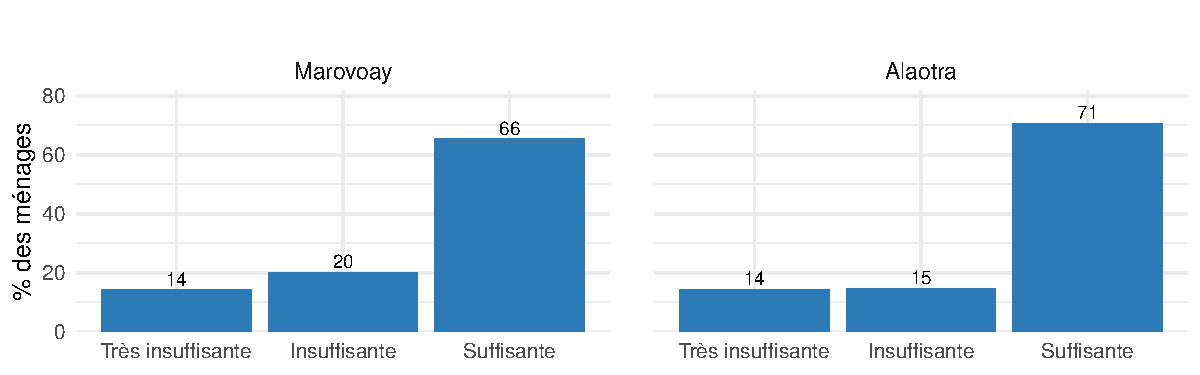
\includegraphics[keepaspectratio]{04_foncier_files/figure-pdf/fig-satisfaction-1.pdf}}

}

\caption{\label{fig-satisfaction}Satisfaction des ménages par rapport à
leur surface foncière}

\end{figure}%

\section{Pistes d'analyse complémentaires}\label{sec-pistes-foncier}

Les données foncières offrent d'autres possibilités d'analyse qui n'ont
pas été développées ici :

\begin{itemize}
\tightlist
\item
  \textbf{Raisons de l'abandon de parcelles} (\texttt{fr30q\_a} à
  \texttt{fr30q\_e}) : cinq variables binaires dont les libellés exacts
  restent à confirmer dans le questionnaire.
\item
  \textbf{Croisement sécurisation × mode d'acquisition} : les parcelles
  héritées sont-elles moins souvent titrées que les parcelles achetées ?
\item
  \textbf{Superficie possédée vs.~superficie exploitée} : reconstituer
  la surface effectivement cultivée par le ménage en combinant
  \texttt{res\_fr30} et \texttt{res\_fr34}.
\item
  \textbf{Rentes perçues sur les parcelles cédées} (\texttt{fr33m1},
  \texttt{fr33m2}, \texttt{fr33n}) : montants moyens des loyers et parts
  de métayage perçus.
\item
  \textbf{Nom sur le titre/certificat} (\texttt{fr30k}, \texttt{fr30m})
  : la correspondance entre le titulaire du document et le propriétaire
  déclaré mériterait une analyse genrée.
\end{itemize}

\bookmarksetup{startatroot}

\chapter{Agriculture, élevage et
pêche}\label{agriculture-uxe9levage-et-puxeache}

Ce chapitre analyse les activités agricoles, d'élevage, de chasse et de
pêche des ménages des deux observatoires. Le chapitre sur les revenus
présente déjà les contributions de ces activités au revenu total ; ici
nous nous intéressons aux pratiques, aux facteurs de production et aux
performances.

\begin{tcolorbox}[enhanced jigsaw, colframe=quarto-callout-warning-color-frame, colback=white, titlerule=0mm, colbacktitle=quarto-callout-warning-color!10!white, toptitle=1mm, opacitybacktitle=0.6, title=\textcolor{quarto-callout-warning-color}{\faExclamationTriangle}\hspace{0.5em}{Travail de vérification en cours}, left=2mm, leftrule=.75mm, bottomtitle=1mm, coltitle=black, arc=.35mm, rightrule=.15mm, bottomrule=.15mm, toprule=.15mm, opacityback=0, breakable]

Les résultats présentés ci-dessous sont provisoires, et sont
susceptibles de faire l'objet de corrections.

\end{tcolorbox}

\section{Agriculture}\label{sec-agriculture}

\subsection{Riziculture}\label{sec-riziculture}

La riziculture est l'activité agricole dominante dans les deux
observatoires.

\textbf{Alaotra.} 58.3 \% des ménages pratiquent la riziculture. Les
riziculteurs exploitent en moyenne 1.4 parcelles (superficie moyenne de
57 ares).

\textbf{Marovoay.} 73.6 \% des ménages pratiquent la riziculture. Les
riziculteurs exploitent en moyenne 1.7 parcelles (superficie moyenne de
68 ares).

\begin{table}

\caption{\label{tbl-pratique-riz}Pratique de la riziculture par
observatoire (\% des ménages)}

\centering{

\caption*{
{\fontsize{20}{25}\selectfont  Pratique de la riziculture\fontsize{12}{15}\selectfont }
} 
\fontsize{12.0pt}{14.0pt}\selectfont
\begin{tabular*}{\linewidth}{@{\extracolsep{\fill}}lrrr}
\toprule
Observatory & Nb ménages & Pratiquent (nb) & Pratiquent (\%) \\ 
\midrule\addlinespace[2.5pt]
Alaotra & 507 & 295 & 58.2 \\ 
Marovoay & 519 & 382 & 73.6 \\ 
\bottomrule
\end{tabular*}

}

\end{table}%

\subsubsection{Mode de faire valoir et accès à
l'eau}\label{mode-de-faire-valoir-et-accuxe8s-uxe0-leau}

La location et le métayage, qui témoignent d'un marché foncier actif,
sont plus ou moins répandus selon l'observatoire.

\textbf{Alaotra.} Le mode de faire valoir dominant est le faire valoir
direct (59.7 \% des parcelles).

\textbf{Marovoay.} Le mode de faire valoir dominant est le faire valoir
direct (46.5 \% des parcelles).

\begin{figure}

\centering{

\pandocbounded{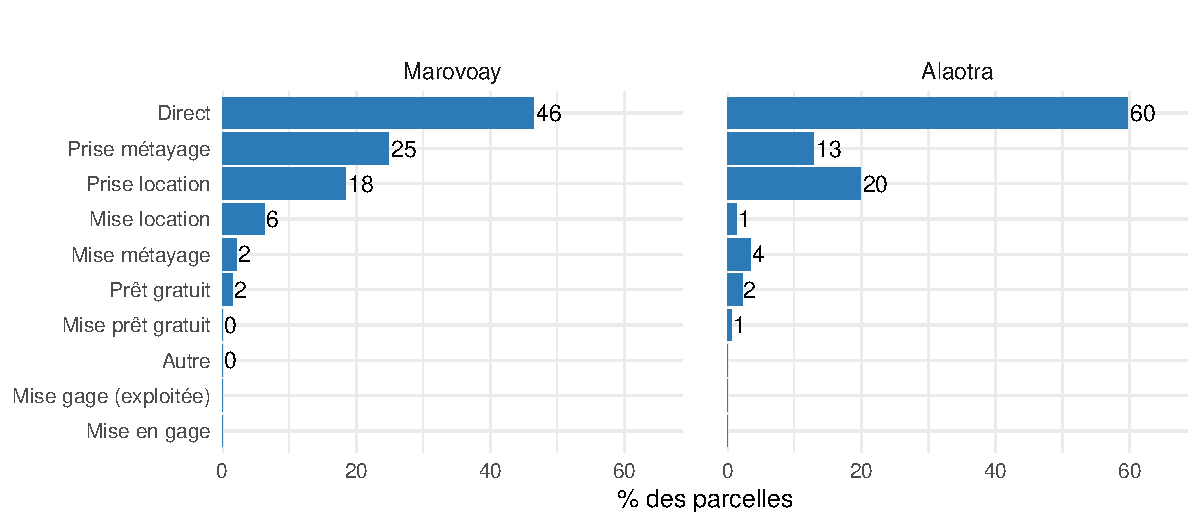
\includegraphics[keepaspectratio]{05_agriculture_files/figure-pdf/fig-tenure-riz-1.pdf}}

}

\caption{\label{fig-tenure-riz}Mode de faire valoir des parcelles
rizicoles par observatoire}

\end{figure}%

La gestion de l'eau est un enjeu central de la riziculture.

\begin{figure}

\centering{

\pandocbounded{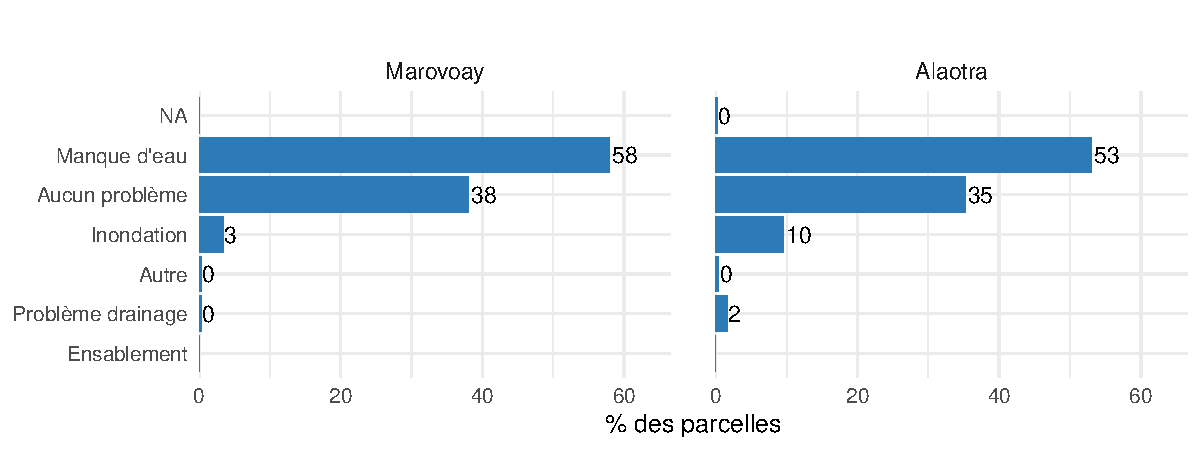
\includegraphics[keepaspectratio]{05_agriculture_files/figure-pdf/fig-eau-riz-1.pdf}}

}

\caption{\label{fig-eau-riz}Problèmes de maîtrise de l'eau sur les
parcelles rizicoles}

\end{figure}%

\subsubsection{Techniques culturales et
intrants}\label{techniques-culturales-et-intrants}

Le choix de la technique est étroitement lié aux conditions
hydrologiques, à la topographie et à l'accès aux intrants.

\textbf{Alaotra.} La technique culturale prédominante est le repiquage
traditionnel (56 \% des parcelles).

\textbf{Marovoay.} La technique culturale prédominante est le repiquage
traditionnel (97 \% des parcelles).

\begin{figure}

\centering{

\pandocbounded{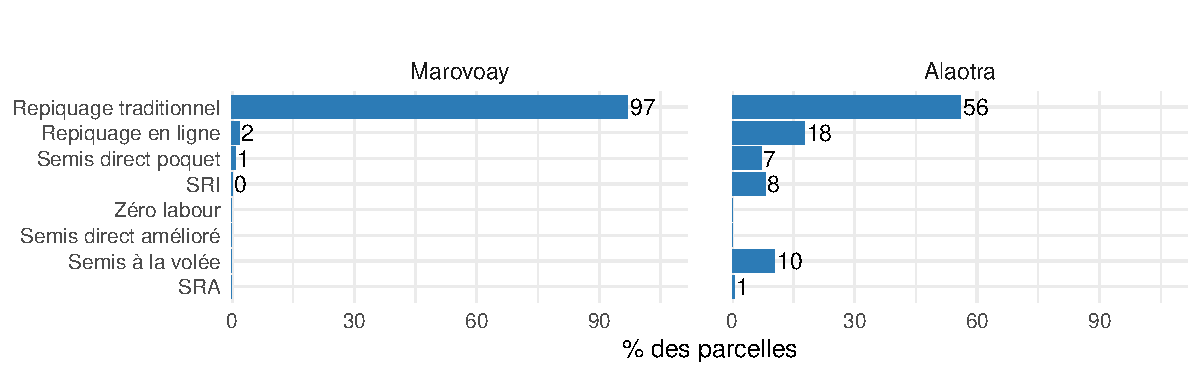
\includegraphics[keepaspectratio]{05_agriculture_files/figure-pdf/fig-technique-riz-1.pdf}}

}

\caption{\label{fig-technique-riz}Technique de culture rizicole par
observatoire}

\end{figure}%

\begin{figure}

\centering{

\pandocbounded{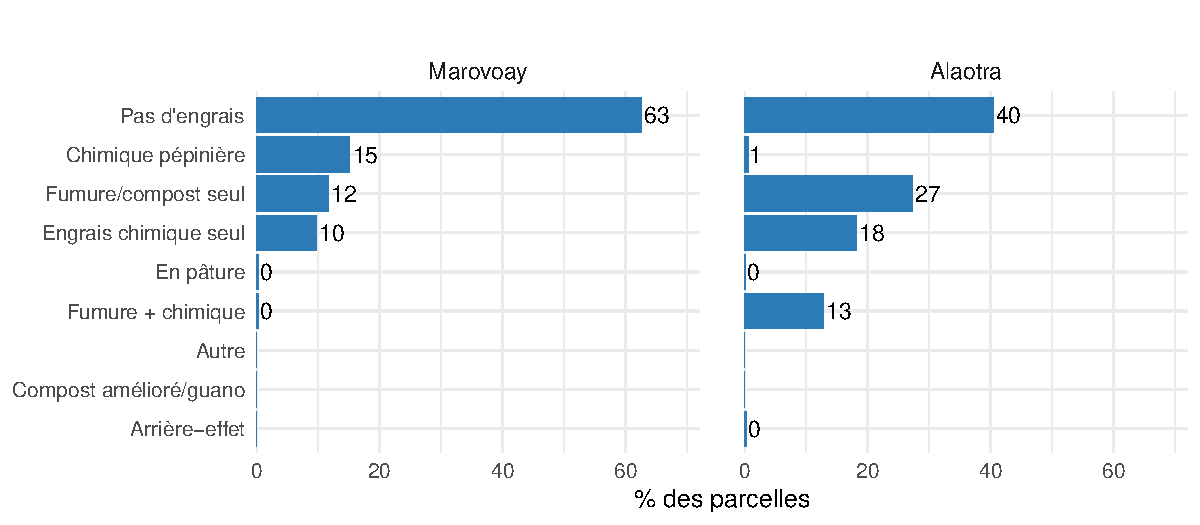
\includegraphics[keepaspectratio]{05_agriculture_files/figure-pdf/fig-engrais-riz-1.pdf}}

}

\caption{\label{fig-engrais-riz}Utilisation d'engrais sur les parcelles
rizicoles}

\end{figure}%

\begin{table}

\caption{\label{tbl-semences-labour}Type de semences et mode de travail
du sol (\% des parcelles)}

\centering{

\caption*{
{\fontsize{20}{25}\selectfont  Semences et travail du sol sur les parcelles rizicoles\fontsize{12}{15}\selectfont }
} 
\fontsize{12.0pt}{14.0pt}\selectfont
\begin{tabular*}{\linewidth}{@{\extracolsep{\fill}}llrr}
\toprule
Indicateur & Modalite & Alaotra & Marovoay \\ 
\midrule\addlinespace[2.5pt]
Semences & Amélioré & 17.6 & 9.2 \\ 
Semences & Traditionnel & 82.4 & 90.8 \\ 
Travail du sol & Angady & 14.9 & 6.7 \\ 
Travail du sol & Charrue & 57.1 & 78.3 \\ 
Travail du sol & Nettoyage (mikaoka) & 0.2 & 6.2 \\ 
Travail du sol & Tracteur/motoculteur & 21.7 & 3.7 \\ 
Travail du sol & Piétinage & 5.3 & 4.9 \\ 
Travail du sol & Autre & 0.8 & 0.1 \\ 
\bottomrule
\end{tabular*}

}

\end{table}%

\subsubsection{Rendements et production}\label{rendements-et-production}

Le rendement rizicole reflète à la fois les conditions agro-écologiques
locales et le degré d'intensification des pratiques.

\textbf{Alaotra.} Le rendement rizicole médian s'établit à 2.5 t/ha
(hors 5 \% des valeurs extrêmes).

\textbf{Marovoay.} Le rendement rizicole médian s'établit à 1.2 t/ha
(hors 5 \% des valeurs extrêmes).

\begin{table}

\caption{\label{tbl-rendement-riz}Perception des rendements rizicoles
par observatoire}

\centering{

\caption*{
{\fontsize{20}{25}\selectfont  Comment jugez-vous le rendement de cette campagne ? (\% des riziculteurs)\fontsize{12}{15}\selectfont }
} 
\fontsize{12.0pt}{14.0pt}\selectfont
\begin{tabular*}{\linewidth}{@{\extracolsep{\fill}}lrr}
\toprule
Perception & Alaotra & Marovoay \\ 
\midrule\addlinespace[2.5pt]
Bon & 20.2 & 12.1 \\ 
Mauvais & 37.7 & 46.4 \\ 
Très bon & 1.0 & 1.3 \\ 
Très mauvais & 41.1 & 40.2 \\ 
\bottomrule
\end{tabular*}

}

\end{table}%

\begin{figure}

\centering{

\pandocbounded{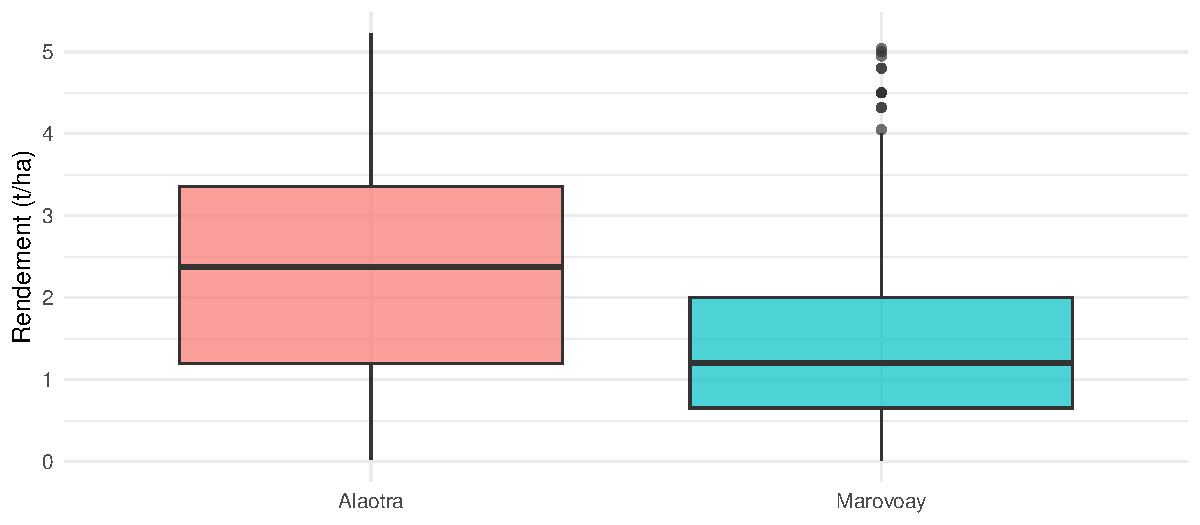
\includegraphics[keepaspectratio]{05_agriculture_files/figure-pdf/fig-rendement-riz-tha-1.pdf}}

}

\caption{\label{fig-rendement-riz-tha}Distribution des rendements
rizicoles (t/ha) par observatoire}

\end{figure}%

\begin{figure}

\centering{

\pandocbounded{
\includegraphics[keepaspectratio]{05_agriculture_files/figure-pdf/fig-production-riz-1.pdf}}

}

\caption{\label{fig-production-riz}Distribution de la production de
paddy par parcelle (kg)}

\end{figure}%

\subsubsection{Topographie et saison de
culture}\label{topographie-et-saison-de-culture}

La position topographique de la parcelle (bas-fond, plaine, tanety)
détermine en grande partie les possibilités de maîtrise de l'eau et le
calendrier cultural. La répartition des saisons de culture reflète les
stratégies d'adaptation des riziculteurs à la variabilité
pluviométrique.

\begin{figure}

\centering{

\pandocbounded{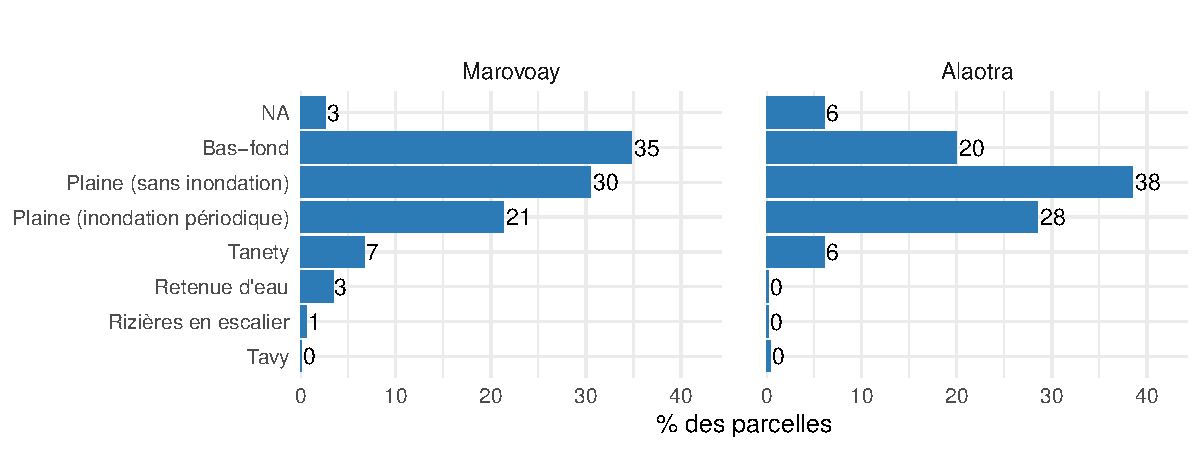
\includegraphics[keepaspectratio]{05_agriculture_files/figure-pdf/fig-topographie-riz-1.pdf}}

}

\caption{\label{fig-topographie-riz}Topographie des parcelles rizicoles}

\end{figure}%

\begin{figure}

\centering{

\pandocbounded{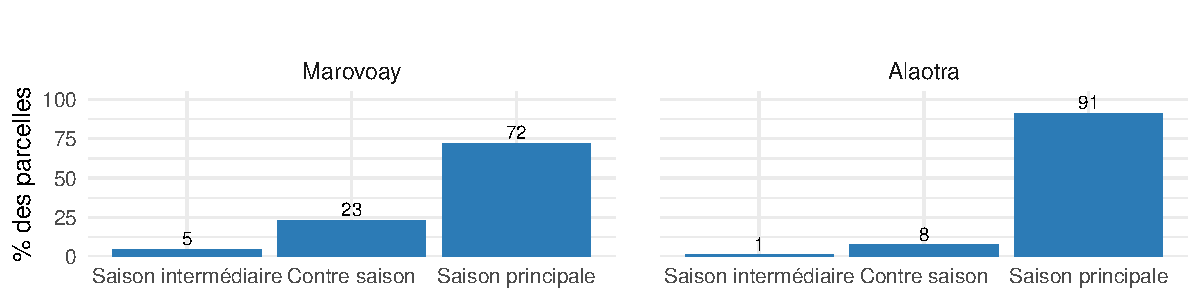
\includegraphics[keepaspectratio]{05_agriculture_files/figure-pdf/fig-saison-riz-1.pdf}}

}

\caption{\label{fig-saison-riz}Saison de culture rizicole}

\end{figure}%

\begin{figure}

\centering{

\pandocbounded{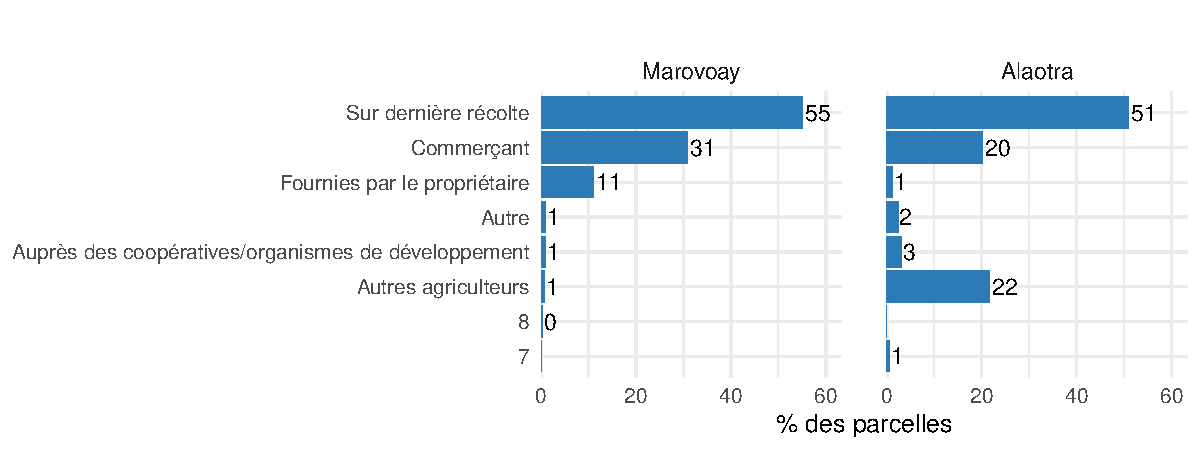
\includegraphics[keepaspectratio]{05_agriculture_files/figure-pdf/fig-origine-semence-1.pdf}}

}

\caption{\label{fig-origine-semence}Origine des semences de riz}

\end{figure}%

\subsubsection{Ventes de riz}\label{ventes-de-riz}

La commercialisation du paddy est une source de revenu majeure. Le
calendrier et le prix de vente sont déterminants pour le revenu rizicole
net.

\textbf{Alaotra.} 41.7 \% des ménages déclarent avoir vendu du riz au
cours de la campagne.

\textbf{Marovoay.} 44.2 \% des ménages déclarent avoir vendu du riz au
cours de la campagne.

\begin{table}

\caption{\label{tbl-ventes-riz-taux}Taux de vente de riz par
observatoire}

\centering{

\caption*{
{\fontsize{20}{25}\selectfont  Vente de riz (paddy ou blanc)\fontsize{12}{15}\selectfont }
} 
\fontsize{12.0pt}{14.0pt}\selectfont
\begin{tabular*}{\linewidth}{@{\extracolsep{\fill}}lrrr}
\toprule
Observatory & Nb ménages & Ont vendu (nb) & Ont vendu (\%) \\ 
\midrule\addlinespace[2.5pt]
Alaotra & 507 & 208 & 41.0 \\ 
Marovoay & 519 & 228 & 43.9 \\ 
\bottomrule
\end{tabular*}

}

\end{table}%

\begin{figure}

\centering{

\pandocbounded{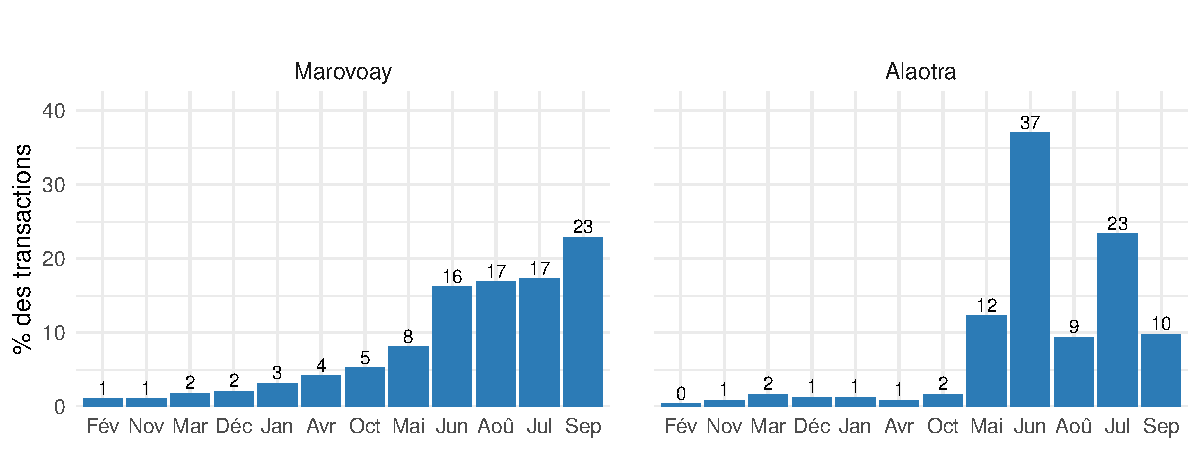
\includegraphics[keepaspectratio]{05_agriculture_files/figure-pdf/fig-ventes-riz-mois-1.pdf}}

}

\caption{\label{fig-ventes-riz-mois}Répartition mensuelle des ventes de
riz}

\end{figure}%

\begin{figure}

\centering{

\pandocbounded{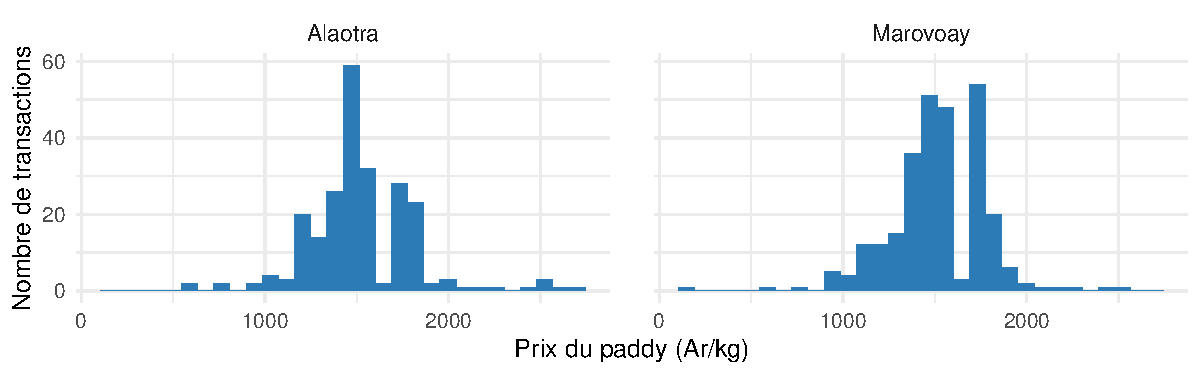
\includegraphics[keepaspectratio]{05_agriculture_files/figure-pdf/fig-prix-paddy-1.pdf}}

}

\caption{\label{fig-prix-paddy}Distribution du prix de vente du paddy
(Ar/kg)}

\end{figure}%

\subsubsection{Bilan rizicole du
ménage}\label{bilan-rizicole-du-muxe9nage}

Le bilan rizicole reconstitue les flux de paddy au niveau du ménage :
stock initial, production, transactions (achat, vente, rente, dons),
autoconsommation alimentaire, utilisation en semences, et stock final.

\begin{table}

\caption{\label{tbl-bilan-riz}Bilan rizicole moyen par ménage (kg de
paddy)}

\centering{

\caption*{
{\fontsize{20}{25}\selectfont  Bilan rizicole moyen par ménage (kg de paddy)\fontsize{12}{15}\selectfont }
} 
\fontsize{12.0pt}{14.0pt}\selectfont
\begin{tabular*}{\linewidth}{@{\extracolsep{\fill}}lrr}
\toprule
Poste & Alaotra & Marovoay \\ 
\midrule\addlinespace[2.5pt]
Stock début campagne & 134 & 100 \\ 
Production totale & 2,164 & 1,977 \\ 
Rente perçue en nature & 206 & 17 \\ 
Achat de paddy & 4 & 16 \\ 
Paddy reçu (dons, héritage\textellipsis) & 116 & 75 \\ 
Vente de paddy & 1,218 & 759 \\ 
Rente versée en nature & 200 & 152 \\ 
Paddy donné / cédé & 34 & 4 \\ 
Alimentation du ménage & 444 & 490 \\ 
Paiement MO en nature & 4 & 39 \\ 
Semences utilisées & 47 & 2 \\ 
Stock fin campagne & 513 & 626 \\ 
\bottomrule
\end{tabular*}

}

\end{table}%

\subsection{Autres cultures}\label{sec-autres-cultures}

La diversification culturale est un enjeu central pour la résilience
alimentaire et économique des ménages.

\textbf{Alaotra.} Au-delà du riz, 52 \% des ménages pratiquent au moins
une culture non rizicole.

\textbf{Marovoay.} Au-delà du riz, 28.8 \% des ménages pratiquent au
moins une culture non rizicole.

\begin{table}

\caption{\label{tbl-pratique-autres}Pratique des cultures non rizicoles}

\centering{

\caption*{
{\fontsize{20}{25}\selectfont  Pratique des cultures non rizicoles\fontsize{12}{15}\selectfont }
} 
\fontsize{12.0pt}{14.0pt}\selectfont
\begin{tabular*}{\linewidth}{@{\extracolsep{\fill}}lrrr}
\toprule
Observatory & Nb ménages & Pratiquent (nb) & Pratiquent (\%) \\ 
\midrule\addlinespace[2.5pt]
Alaotra & 507 & 262 & 51.7 \\ 
Marovoay & 519 & 149 & 28.7 \\ 
\bottomrule
\end{tabular*}

}

\end{table}%

\subsubsection{Diversification et principales
cultures}\label{diversification-et-principales-cultures}

Le portefeuille de cultures reflète les opportunités de marché et les
conditions pédoclimatiques propres à chaque observatoire.

\textbf{Alaotra.} Les ménages cultivent un nombre médian de 1 cultures
non rizicoles.

\textbf{Marovoay.} Les ménages cultivent un nombre médian de 1 cultures
non rizicoles.

\begin{figure}

\centering{

\pandocbounded{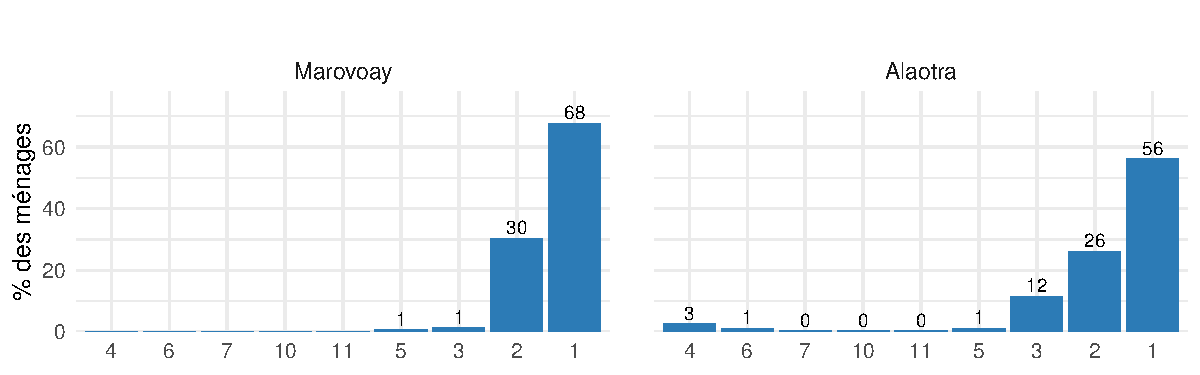
\includegraphics[keepaspectratio]{05_agriculture_files/figure-pdf/fig-diversification-1.pdf}}

}

\caption{\label{fig-diversification}Nombre de cultures non rizicoles par
ménage}

\end{figure}%

\begin{figure}

\centering{

\pandocbounded{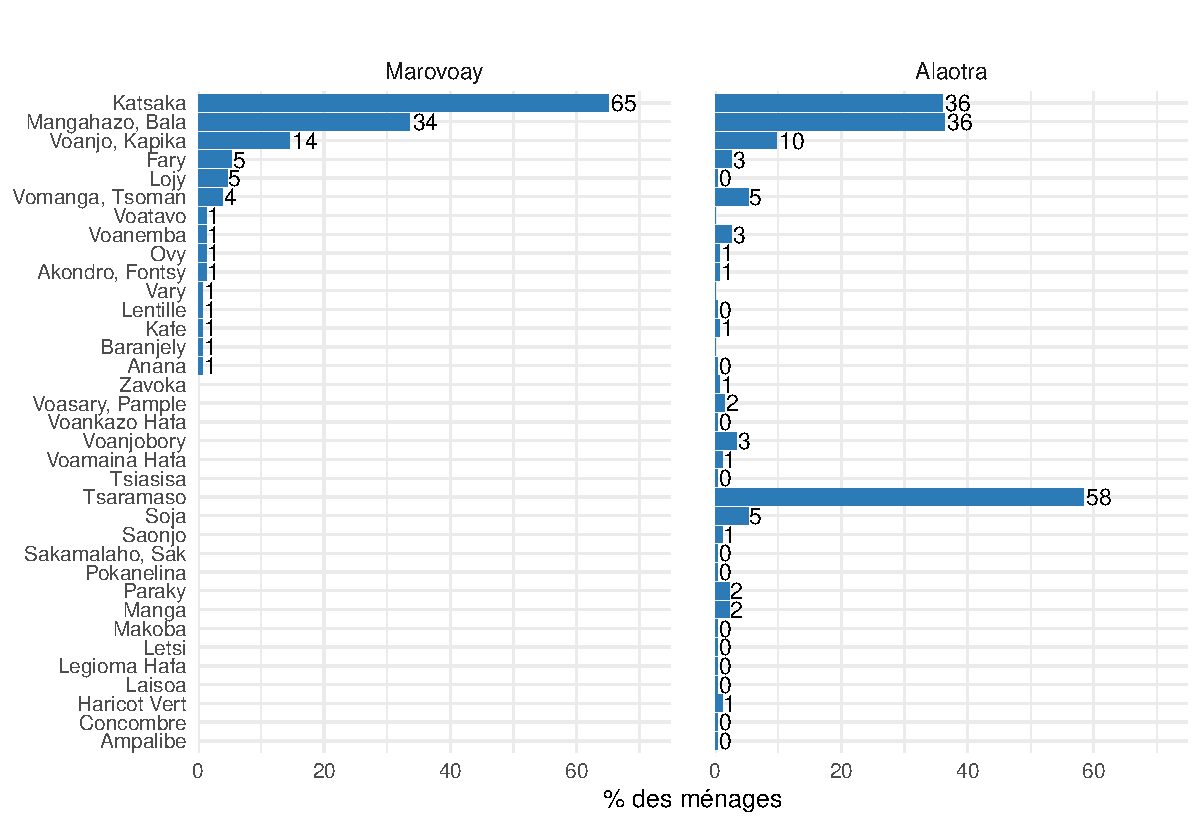
\includegraphics[keepaspectratio]{05_agriculture_files/figure-pdf/fig-top-cultures-1.pdf}}

}

\caption{\label{fig-top-cultures}Cultures non rizicoles les plus
fréquentes (nb de ménages pratiquant)}

\end{figure}%

\subsubsection{Fertilisation et production des autres
cultures}\label{fertilisation-et-production-des-autres-cultures}

L'accès aux engrais (organiques et chimiques) est un facteur déterminant
de la productivité des cultures non rizicoles. Les pratiques de
fertilisation diffèrent sensiblement entre les deux observatoires en
raison de l'accessibilité et du coût des intrants.

\begin{figure}

\centering{

\pandocbounded{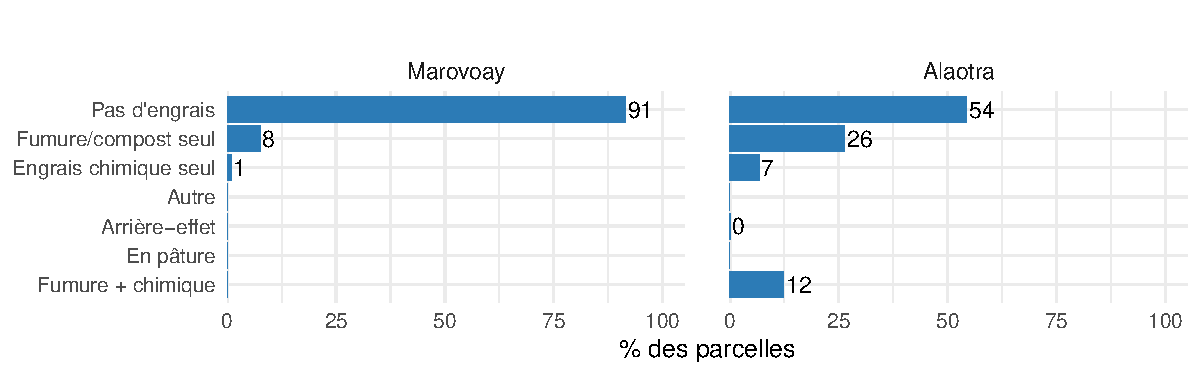
\includegraphics[keepaspectratio]{05_agriculture_files/figure-pdf/fig-engrais-autres-1.pdf}}

}

\caption{\label{fig-engrais-autres}Utilisation d'engrais sur les
parcelles de cultures non rizicoles}

\end{figure}%

\begin{table}

\caption{\label{tbl-production-autres}Production et ventes des
principales cultures non rizicoles}

\centering{

\caption*{
{\fontsize{20}{25}\selectfont  Production et ventes des principales cultures non rizicoles\fontsize{12}{15}\selectfont }
} 
\fontsize{12.0pt}{14.0pt}\selectfont
\begin{tabular*}{\linewidth}{@{\extracolsep{\fill}}llrrrr}
\toprule
Observatory & Culture & Nb parcelles & Production moy. (kg) & \% vendu (moy.) & Montant vente moy. (Ar) \\ 
\midrule\addlinespace[2.5pt]
Alaotra & Tsaramaso & 145 & 105 & 62.3 & 234,486 \\ 
Alaotra & Mangahazo, Bala & 94 & 253 & 27.0 & 113,707 \\ 
Alaotra & Katsaka & 93 & 140 & 24.8 & 199,969 \\ 
Alaotra & Voanjo, Kapika & 26 & 167 & 47.8 & 192,875 \\ 
Alaotra & Vomanga, Tsoman & 14 & 160 & 27.1 & 39,429 \\ 
Alaotra & Soja & 12 & 83 & 86.5 & 174,182 \\ 
Alaotra & Voanjobory & 8 & 324 & 60.8 & 570,000 \\ 
Alaotra & Fary & 7 & 1,629 & 87.9 & 354,286 \\ 
Alaotra & Voanemba & 7 & 45 & 69.9 & 106,333 \\ 
Alaotra & Manga & 6 & 410 & 15.8 & 540,000 \\ 
Alaotra & Paraky & 6 & 148 & 66.0 & 80,000 \\ 
Marovoay & Katsaka & 93 & 351 & 29.2 & 390,936 \\ 
Marovoay & Mangahazo, Bala & 38 & 272 & 39.0 & 201,771 \\ 
Marovoay & Voanjo, Kapika & 23 & 366 & 56.7 & 327,621 \\ 
Marovoay & Fary & 8 & 1,582 & 90.8 & 272,750 \\ 
Marovoay & Lojy & 6 & 354 & 55.7 & 682,500 \\ 
Marovoay & Vomanga, Tsoman & 6 & 7,146 & 36.7 & 5,260,000 \\ 
\bottomrule
\end{tabular*}

}

\end{table}%

\subsubsection{Perception des
rendements}\label{perception-des-rendements}

Au-delà des mesures quantitatives, la perception subjective des
rendements par les agriculteurs constitue un indicateur complémentaire
de la performance de la campagne. Elle reflète à la fois les résultats
objectifs et les attentes des producteurs.

\begin{table}

\caption{\label{tbl-rendement-autres}Perception des rendements des
cultures non rizicoles}

\centering{

\caption*{
{\fontsize{20}{25}\selectfont  Perception des rendements des cultures non rizicoles (\% des pratiquants)\fontsize{12}{15}\selectfont }
} 
\fontsize{12.0pt}{14.0pt}\selectfont
\begin{tabular*}{\linewidth}{@{\extracolsep{\fill}}llrr}
\toprule
Indicateur & Modalite & Alaotra & Marovoay \\ 
\midrule\addlinespace[2.5pt]
Rendement cette campagne & Bon & 35.1 & 20.1 \\ 
Rendement cette campagne & Mauvais & 46.7 & 53.0 \\ 
Rendement cette campagne & Très bon & 2.7 & 0.7 \\ 
Rendement cette campagne & Très mauvais & 15.4 & 26.2 \\ 
Par rapport a l'an dernier & Augmenté & 24.4 & 8.2 \\ 
Par rapport a l'an dernier & Diminué & 54.3 & 49.7 \\ 
Par rapport a l'an dernier & Inchangé & 21.3 & 41.5 \\ 
Par rapport a l'an dernier & 4 & 0.0 & 0.7 \\ 
\bottomrule
\end{tabular*}

}

\end{table}%

\subsection{Jardins potagers et cueillette}\label{sec-jardins}

Les jardins potagers et la cueillette de produits sauvages complètent
les activités agricoles des ménages. Ils jouent un rôle important dans
la diversification alimentaire, en particulier pendant la période de
soudure.

\begin{table}

\caption{\label{tbl-jardin-pratique}Pratique du jardin potager et de la
cueillette}

\centering{

\caption*{
{\fontsize{20}{25}\selectfont  Taux de pratique (\% des ménages)\fontsize{12}{15}\selectfont }
} 
\fontsize{12.0pt}{14.0pt}\selectfont
\begin{tabular*}{\linewidth}{@{\extracolsep{\fill}}lrrr}
\toprule
Activité & Alaotra & Marovoay & Total \\ 
\midrule\addlinespace[2.5pt]
Jardin potager & 70 & 46 & 58 \\ 
Exploitation forestière & 54 & 36 & 45 \\ 
\bottomrule
\end{tabular*}

}

\end{table}%

\begin{figure}

\centering{

\pandocbounded{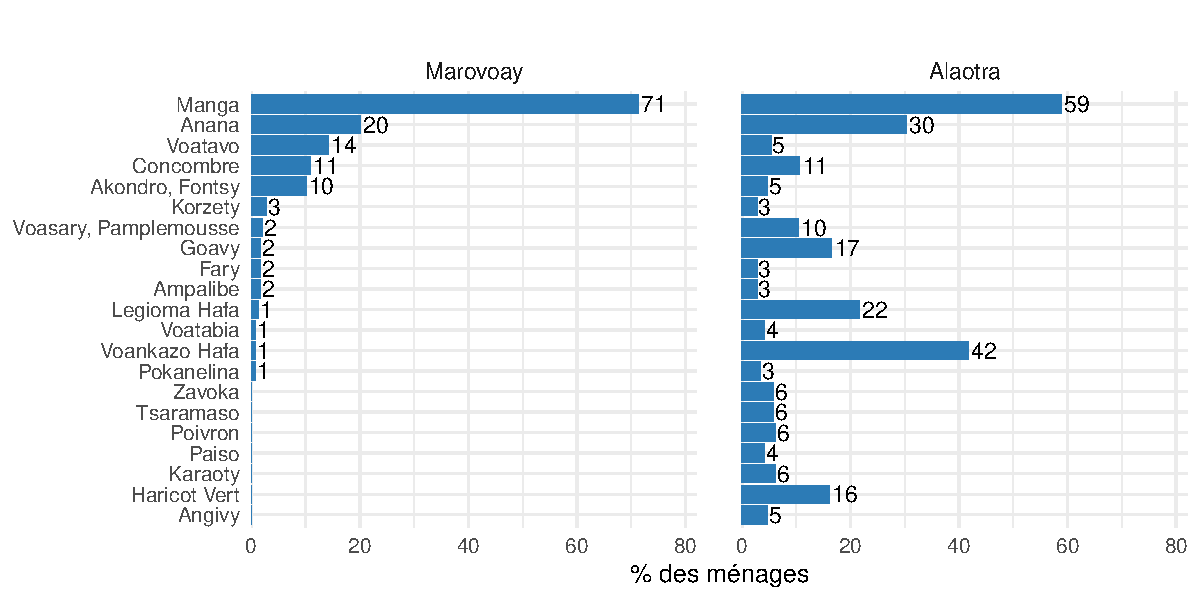
\includegraphics[keepaspectratio]{05_agriculture_files/figure-pdf/fig-top-jardin-1.pdf}}

}

\caption{\label{fig-top-jardin}Produits de jardin / cueillette les plus
fréquents}

\end{figure}%

\subsection{Exploitation forestière}\label{sec-foret}

L'exploitation des ressources forestières (bois de chauffe, charbon,
bois d'œuvre, plantes médicinales) constitue une activité complémentaire
pour de nombreux ménages. Les produits forestiers sont essentiels à la
fois comme source d'énergie domestique et comme revenu d'appoint.

\begin{figure}

\centering{

\pandocbounded{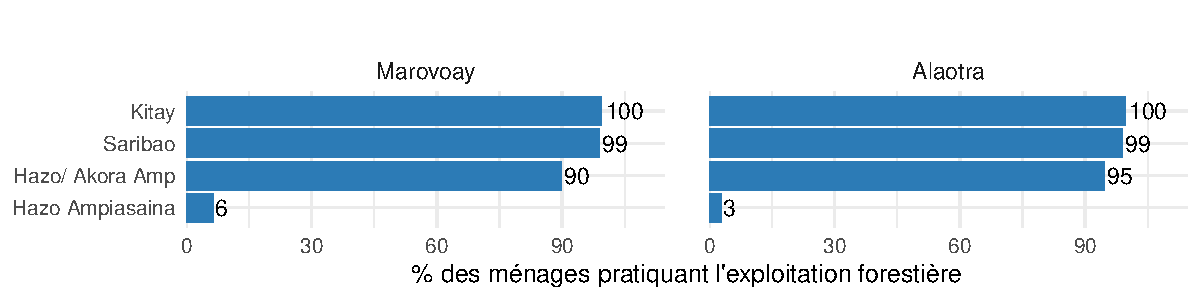
\includegraphics[keepaspectratio]{05_agriculture_files/figure-pdf/fig-produits-foret-1.pdf}}

}

\caption{\label{fig-produits-foret}Principaux produits de l'exploitation
forestière}

\end{figure}%

\section{Élevage}\label{sec-elevage}

\subsection{Pratique de l'élevage}\label{pratique-de-luxe9levage}

L'élevage remplit des fonctions multiples : épargne sur pied, force de
travail, autoconsommation et source de revenu.

\textbf{Alaotra.} L'élevage est pratiqué par 65.4 \% des ménages.

\textbf{Marovoay.} L'élevage est pratiqué par 72.3 \% des ménages.

\begin{table}

\caption{\label{tbl-elevage-pratique}Taux de pratique de l'élevage}

\centering{

\caption*{
{\fontsize{20}{25}\selectfont  Pratique de l'élevage\fontsize{12}{15}\selectfont }
} 
\fontsize{12.0pt}{14.0pt}\selectfont
\begin{tabular*}{\linewidth}{@{\extracolsep{\fill}}lrrr}
\toprule
Observatory & Nb ménages & Pratiquent (nb) & Pratiquent (\%) \\ 
\midrule\addlinespace[2.5pt]
Alaotra & 507 & 331 & 65.3 \\ 
Marovoay & 519 & 374 & 72.1 \\ 
\bottomrule
\end{tabular*}

}

\end{table}%

\subsection{Espèces élevées}\label{espuxe8ces-uxe9levuxe9es}

Le choix des espèces reflète les conditions agro-écologiques, les
traditions locales et les opportunités de marché.

\textbf{Alaotra.} L'espèce la plus élevée est le Kisoa.

\textbf{Marovoay.} L'espèce la plus élevée est le Omby Miasa.

\begin{figure}

\centering{

\pandocbounded{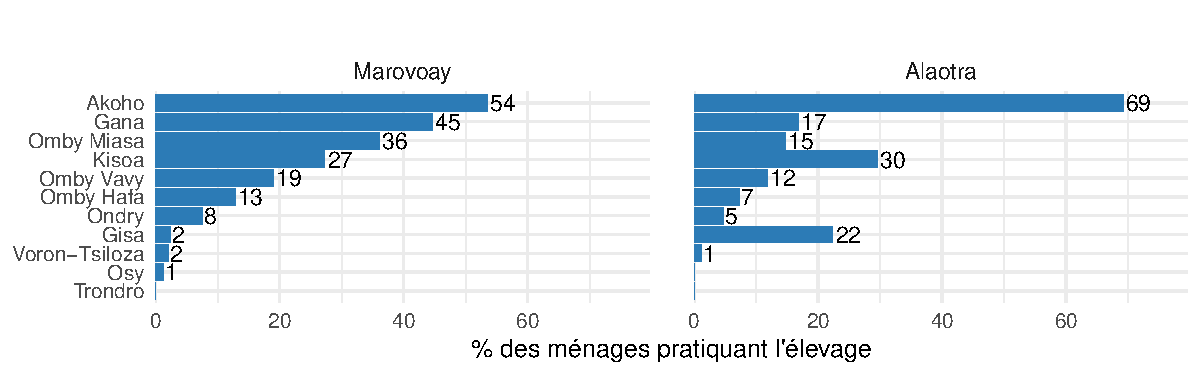
\includegraphics[keepaspectratio]{05_agriculture_files/figure-pdf/fig-especes-elevage-1.pdf}}

}

\caption{\label{fig-especes-elevage}Espèces élevées (nombre de ménages
pratiquant)}

\end{figure}%

\subsection{Objectifs de l'élevage}\label{objectifs-de-luxe9levage}

L'élevage répond à trois objectifs principaux : l'épargne/assurance
(constitution d'un capital mobilisable en cas de choc),
l'autoconsommation (lait, œufs, viande) et la vente. La hiérarchie de
ces objectifs varie selon l'espèce.

\begin{figure}

\centering{

\pandocbounded{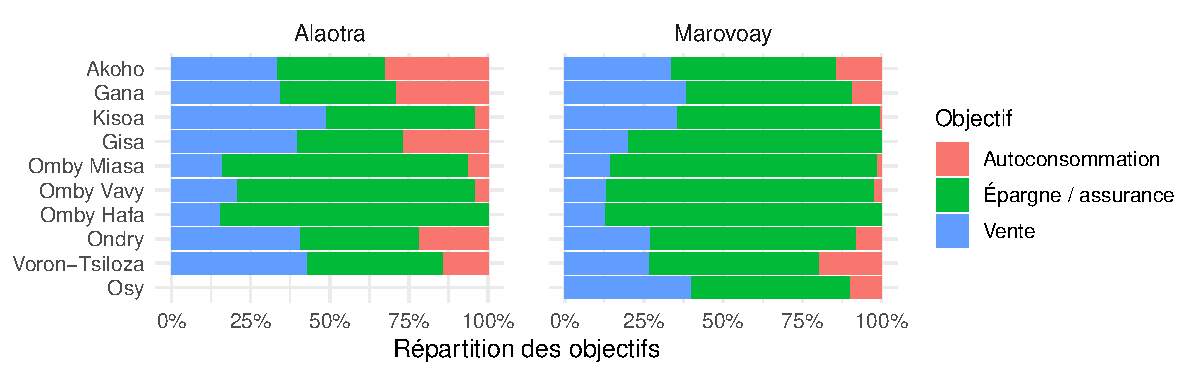
\includegraphics[keepaspectratio]{05_agriculture_files/figure-pdf/fig-objectifs-elevage-1.pdf}}

}

\caption{\label{fig-objectifs-elevage}Objectifs de l'élevage par espèce
(\% des ménages éleveurs)}

\end{figure}%

\subsection{Ventes et pertes d'animaux}\label{ventes-et-pertes-danimaux}

La dynamique du cheptel dépend des entrées (naissances, achats) et des
sorties (ventes, pertes, abattages). Les pertes d'animaux, liées aux
maladies, au vol ou aux catastrophes naturelles, représentent un risque
économique majeur pour les éleveurs.

\begin{table}

\caption{\label{tbl-ventes-elevage}Ventes d'animaux par observatoire}

\centering{

\caption*{
{\fontsize{20}{25}\selectfont  Ventes d'animaux par espèce et observatoire\fontsize{12}{15}\selectfont }
} 
\fontsize{12.0pt}{14.0pt}\selectfont
\begin{tabular*}{\linewidth}{@{\extracolsep{\fill}}llrrr}
\toprule
Observatory & Espece & Nb transactions & Nb animaux vendus & Valeur totale (Ar) \\ 
\midrule\addlinespace[2.5pt]
Alaotra & Gisa & 29 & 269 & 89,771 \\ 
Alaotra & Kisoa & 50 & 80 & 25,625 \\ 
Alaotra & Akoho & 112 & 948 & 22,055 \\ 
Alaotra & Omby Miasa & 4 & 7 & 9,930 \\ 
Alaotra & Gana & 17 & 341 & 6,763 \\ 
Alaotra & Ondry & 7 & 33 & 3,936 \\ 
Alaotra & Omby Vavy & 2 & 3 & 2,580 \\ 
Alaotra & Voron-Tsiloza & 1 & 25 & 1,875 \\ 
Alaotra & Omby Hafa & 2 & 2 & 1,550 \\ 
Marovoay & Akoho & 112 & 778 & 60,200 \\ 
Marovoay & Omby Miasa & 21 & 37 & 45,650 \\ 
Marovoay & Kisoa & 43 & 102 & 36,995 \\ 
Marovoay & Gana & 90 & 1,319 & 19,398 \\ 
Marovoay & Omby Vavy & 7 & 11 & 9,400 \\ 
Marovoay & Omby Hafa & 3 & 5 & 3,859 \\ 
Marovoay & Ondry & 6 & 30 & 3,080 \\ 
Marovoay & Voron-Tsiloza & 3 & 34 & 1,260 \\ 
Marovoay & Osy & 2 & 10 & 1,000 \\ 
Marovoay & Gisa & 2 & 10 & 290 \\ 
\bottomrule
\end{tabular*}

}

\end{table}%

\begin{figure}

\centering{

\pandocbounded{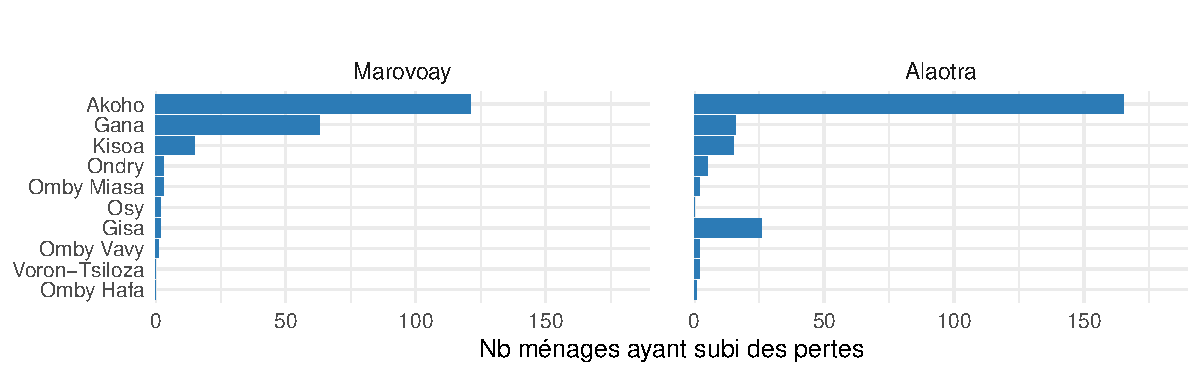
\includegraphics[keepaspectratio]{05_agriculture_files/figure-pdf/fig-pertes-elevage-1.pdf}}

}

\caption{\label{fig-pertes-elevage}Ménages ayant subi des pertes de
bétail}

\end{figure}%

\subsection{Produits de l'élevage}\label{produits-de-luxe9levage}

Outre la vente d'animaux sur pied, l'élevage génère des produits dérivés
(lait, œufs, miel, fumier) qui contribuent à l'alimentation et aux
revenus du ménage.

\begin{table}

\caption{\label{tbl-produits-elevage}Produits de l'élevage : nombre de
ménages producteurs}

\centering{

\caption*{
{\fontsize{20}{25}\selectfont  Produits de l'élevage déclarés par les ménages\fontsize{12}{15}\selectfont }
} 
\fontsize{12.0pt}{14.0pt}\selectfont
\begin{tabular*}{\linewidth}{@{\extracolsep{\fill}}lrrr}
\toprule
Produit & Alaotra & Marovoay & Total \\ 
\midrule\addlinespace[2.5pt]
Ronono & 103 & 98 & 201 \\ 
Atody & 95 & 98 & 193 \\ 
Yaourt/Habobo & 89 & 93 & 182 \\ 
Hena & 87 & 88 & 175 \\ 
Henan'ondry & 2 & 7 & 9 \\ 
Vorona & 1 & 1 & 2 \\ 
Henan-Kisoa & 1 & 0 & 1 \\ 
Trondro Nompian & 0 & 1 & 1 \\ 
\bottomrule
\end{tabular*}

}

\end{table}%

\section{Chasse et pêche}\label{sec-chasse-peche}

La chasse et la pêche constituent des activités complémentaires, souvent
saisonnières, qui contribuent à la diversification alimentaire et au
revenu, en particulier dans les zones proches des plans d'eau.

\textbf{Alaotra.} Ces activités sont pratiquées par 18.3 \% des ménages.

\textbf{Marovoay.} Ces activités sont pratiquées par 34.5 \% des
ménages.

\begin{table}

\caption{\label{tbl-chasse-peche-pratique}Taux de pratique de la chasse
et de la pêche}

\centering{

\caption*{
{\fontsize{20}{25}\selectfont  Pratique de la chasse et de la pêche (\% des ménages)\fontsize{12}{15}\selectfont }
} 
\fontsize{12.0pt}{14.0pt}\selectfont
\begin{tabular*}{\linewidth}{@{\extracolsep{\fill}}lrrr}
\toprule
Activité & Alaotra & Marovoay & Total \\ 
\midrule\addlinespace[2.5pt]
Chasse / Pêche & 18 & 34 & 27 \\ 
\bottomrule
\end{tabular*}

}

\end{table}%

\begin{figure}

\centering{

\pandocbounded{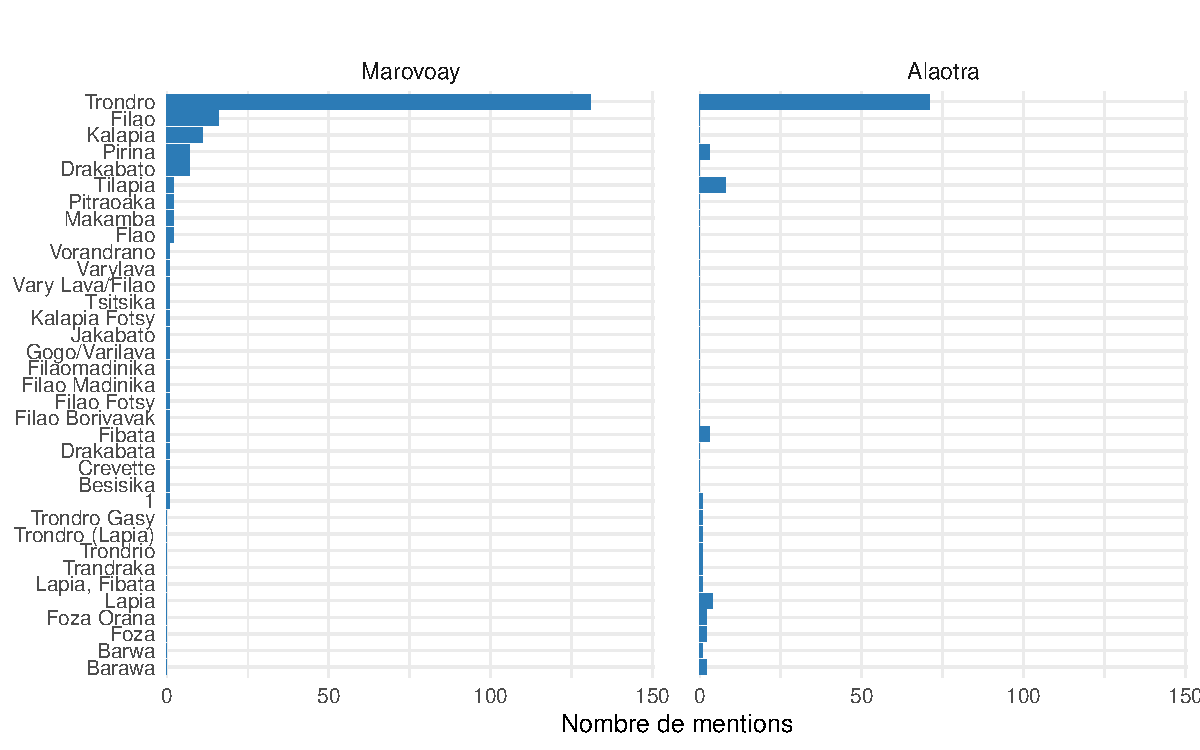
\includegraphics[keepaspectratio]{05_agriculture_files/figure-pdf/fig-chasse-especes-1.pdf}}

}

\caption{\label{fig-chasse-especes}Principales espèces chassées/pêchées}

\end{figure}%

\begin{figure}

\centering{

\pandocbounded{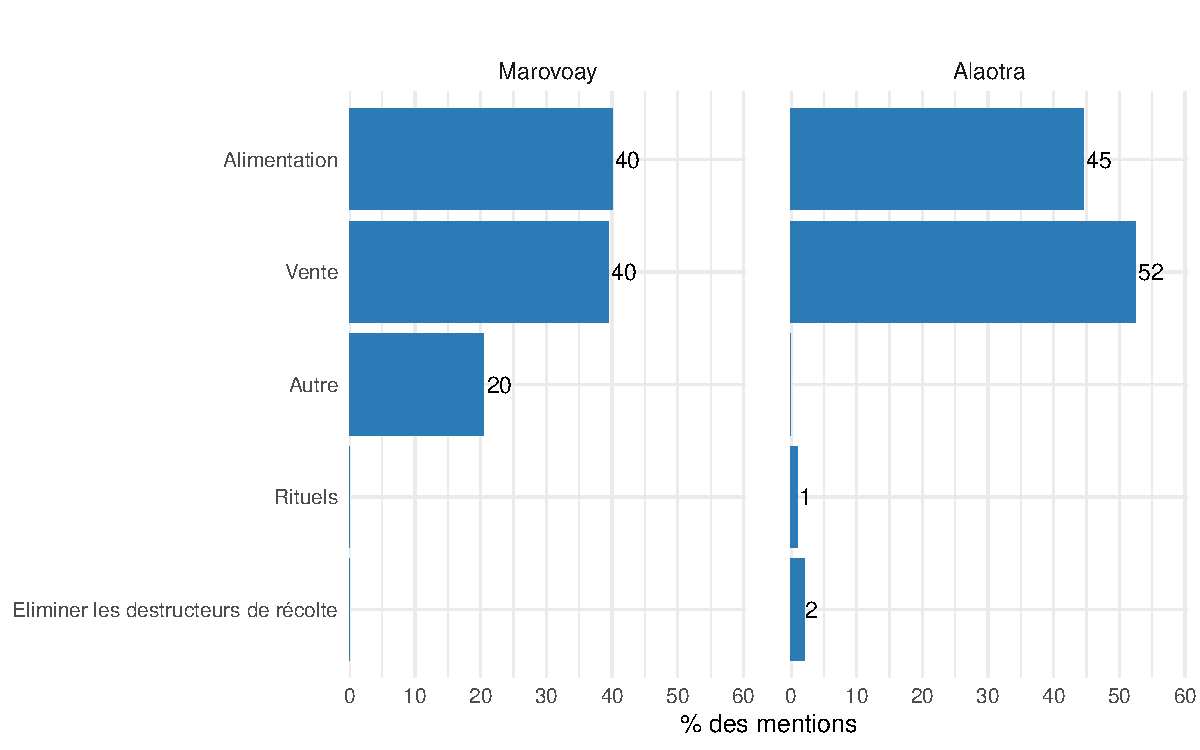
\includegraphics[keepaspectratio]{05_agriculture_files/figure-pdf/fig-chasse-raison-1.pdf}}

}

\caption{\label{fig-chasse-raison}Raisons de la chasse/pêche par
observatoire}

\end{figure}%

\subsection{Fréquence et
saisonnalité}\label{fruxe9quence-et-saisonnalituxe9}

La fréquence de pêche et son calendrier saisonnier dépendent du régime
hydrologique local. Les périodes de hautes eaux correspondent
généralement à une activité de pêche plus intense.

\begin{figure}

\centering{

\pandocbounded{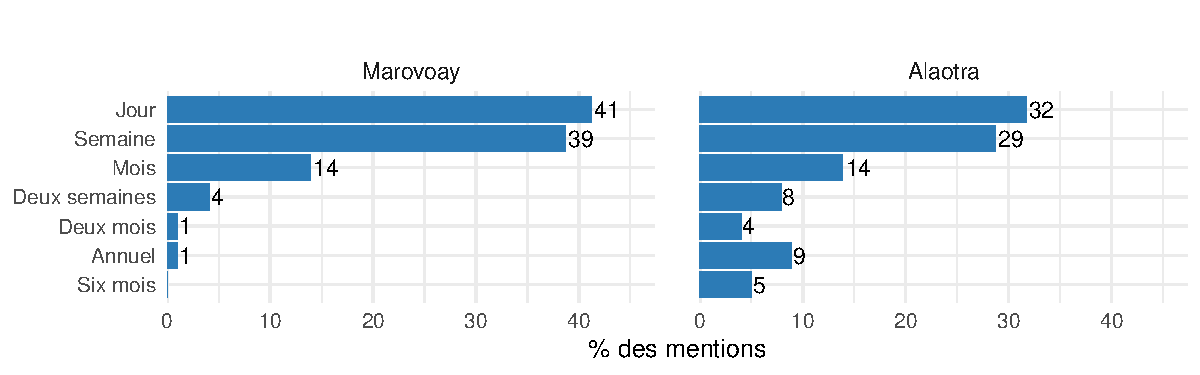
\includegraphics[keepaspectratio]{05_agriculture_files/figure-pdf/fig-frequence-peche-1.pdf}}

}

\caption{\label{fig-frequence-peche}Fréquence de la chasse/pêche}

\end{figure}%

\begin{figure}

\centering{

\pandocbounded{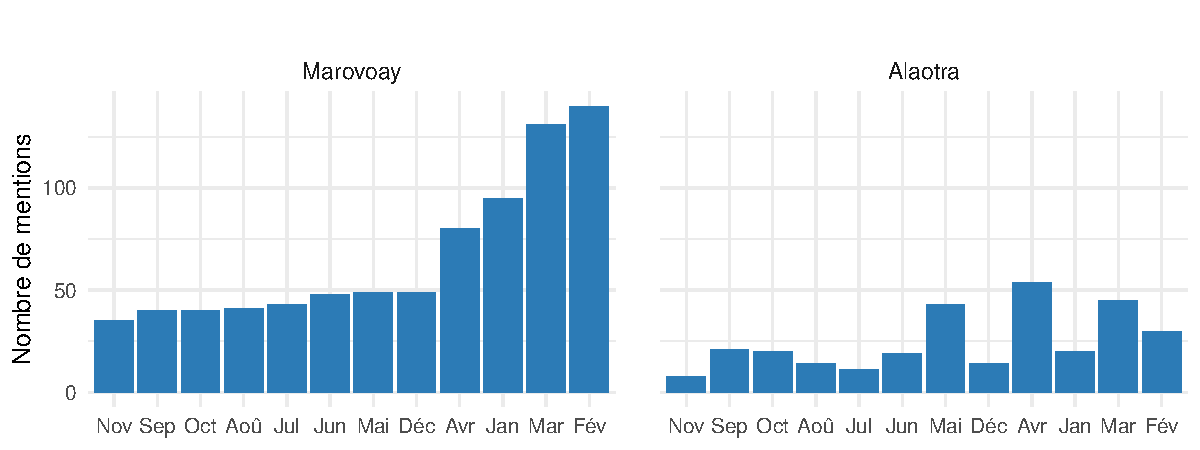
\includegraphics[keepaspectratio]{05_agriculture_files/figure-pdf/fig-saisonnalite-peche-1.pdf}}

}

\caption{\label{fig-saisonnalite-peche}Saisonnalité de la chasse/pêche
(\% de mentions par mois)}

\end{figure}%

\section{Main d'oeuvre agricole}\label{sec-main-oeuvre}

\subsection{Emploi de main d'oeuvre}\label{emploi-de-main-doeuvre}

L'ampleur du recours à la main d'œuvre extérieure dépend de la
superficie cultivée, du type de culture et de la disponibilité de main
d'œuvre familiale.

\textbf{Alaotra.} Le recours à la main d'œuvre extérieure (salariée ou
par entraide) concerne 46.8 \% des ménages.

\textbf{Marovoay.} Le recours à la main d'œuvre extérieure (salariée ou
par entraide) concerne 58.8 \% des ménages.

\begin{table}

\caption{\label{tbl-main-oeuvre-pratique}Recours à la main d'oeuvre
agricole}

\centering{

\caption*{
{\fontsize{20}{25}\selectfont  Recours à la main d'oeuvre agricole (\% des ménages)\fontsize{12}{15}\selectfont }
} 
\fontsize{12.0pt}{14.0pt}\selectfont
\begin{tabular*}{\linewidth}{@{\extracolsep{\fill}}lrrr}
\toprule
Type & Alaotra & Marovoay & Total \\ 
\midrule\addlinespace[2.5pt]
Main d'oeuvre non permanente & 47 & 59 & 53 \\ 
Main d'oeuvre permanente & 7 & 4 & 5 \\ 
\bottomrule
\end{tabular*}

}

\end{table}%

\subsection{Opérations nécessitant de la main d'oeuvre
salariée}\label{opuxe9rations-nuxe9cessitant-de-la-main-doeuvre-salariuxe9e}

Les trois opérations rizicoles principales (travail du sol, sarclage,
moisson) mobilisent des volumes de main d'œuvre différents. Le salaire
journalier et le recours à l'entraide varient sensiblement selon
l'opération et l'observatoire.

\begin{table}

\caption{\label{tbl-operations-mo}Main d'œuvre salariée et entraide par
opération agricole}

\centering{

\fontsize{12.0pt}{14.0pt}\selectfont
\begin{tabular*}{\linewidth}{@{\extracolsep{\fill}}llrrr}
\toprule
Observatory & Operation & Salariee (\%) & Entraide (\%) & Salaire moyen (Ar) \\ 
\midrule\addlinespace[2.5pt]
Alaotra & Moisson & 79.5 & 14.7 & 216,171 \\ 
Marovoay & Moisson & 91.1 & 8.9 & 182,954 \\ 
Alaotra & Sarclage & 64.7 & 21.6 & 229,960 \\ 
Marovoay & Sarclage & 84.6 & 7.2 & 150,626 \\ 
Alaotra & Travail du sol & 69.2 & 15.8 & 194,315 \\ 
Marovoay & Travail du sol & 79.0 & 6.9 & 193,831 \\ 
\bottomrule
\end{tabular*}

}

\end{table}%

\subsection{Main d'oeuvre permanente}\label{main-doeuvre-permanente}

Le recours à la main d'œuvre permanente (salariés employés à l'année)
reste minoritaire et concerne principalement les exploitations les plus
grandes. Les conditions d'emploi (salaire, logement, nourriture)
reflètent le marché du travail agricole local.

\begin{table}

\caption{\label{tbl-main-oeuvre-perm}Caractéristiques de la main
d'oeuvre permanente}

\centering{

\caption*{
{\fontsize{20}{25}\selectfont  Main d'œuvre permanente par type d'activité\fontsize{12}{15}\selectfont }
} 
\fontsize{12.0pt}{14.0pt}\selectfont
\begin{tabular*}{\linewidth}{@{\extracolsep{\fill}}llrrr}
\toprule
Observatory & Activite & Nb employés & Salaire moyen argent (Ar) & Salaire moyen nature (Ar) \\ 
\midrule\addlinespace[2.5pt]
Alaotra & Élevage & 27 & 434,839 & 245,286 \\ 
Alaotra & Riziculture & 18 & 713,368 & 557,625 \\ 
Alaotra & Aide ménagère & 18 & 306,000 & 426,667 \\ 
Alaotra & Autres cultures & 15 & 707,111 & 380,000 \\ 
Alaotra & Autres activités & 6 & 1,166,000 & NaN \\ 
Marovoay & Élevage & 15 & 252,500 & 285,714 \\ 
Marovoay & Aide ménagère & 4 & 445,000 & 0 \\ 
Marovoay & Autres activités & 4 & 907,500 & 0 \\ 
Marovoay & Autres cultures & 1 & 250,000 & NaN \\ 
\bottomrule
\end{tabular*}

}

\end{table}%

\subsection{Cultures non rizicoles par quintile de
revenu}\label{cultures-non-rizicoles-par-quintile-de-revenu}

Les ménages les plus aisés cultivent-ils des cultures différentes ? On
croise ici les familles de cultures avec les quintiles de revenu courant
du ménage.

\begin{figure}

\centering{

\pandocbounded{
\includegraphics[keepaspectratio]{05_agriculture_files/figure-pdf/fig-cultures-quintile-1.pdf}}

}

\caption{\label{fig-cultures-quintile}Familles de cultures non rizicoles
pratiquées selon le quintile de revenu}

\end{figure}%

\begin{table}

\caption{\label{tbl-cultures-quintile}Nombre moyen de cultures non
rizicoles par ménage et quintile de revenu}

\centering{

\caption*{
{\fontsize{20}{25}\selectfont  Diversification des cultures non rizicoles selon le quintile de revenu\fontsize{12}{15}\selectfont }
} 
\fontsize{12.0pt}{14.0pt}\selectfont
\begin{tabular*}{\linewidth}{@{\extracolsep{\fill}}lrrrrrrrrrr}
\toprule
Observatory & n\_men\_Q5 & n\_men\_Q1 & n\_men\_Q4 & n\_men\_Q2 & n\_men\_Q3 & nb\_cult\_moy\_Q5 & nb\_cult\_moy\_Q1 & nb\_cult\_moy\_Q4 & nb\_cult\_moy\_Q2 & nb\_cult\_moy\_Q3 \\ 
\midrule\addlinespace[2.5pt]
Alaotra & 67 & 46 & 58 & 52 & 43 & 2.0 & 1.5 & 1.9 & 1.5 & 1.8 \\ 
Marovoay & 39 & 30 & 29 & 28 & 26 & 1.6 & 1.4 & 1.2 & 1.2 & 1.3 \\ 
\bottomrule
\end{tabular*}

}

\end{table}%

\section{Évolution des indicateurs agricoles
(1995--2025)}\label{sec-agro-multiyear}

Les fichiers rizicoles (\texttt{res\_r}) et d'élevage
(\texttt{res\_el2}) couvrent la quasi-totalité des campagnes depuis
1995. On retrace ici l'évolution de la production rizicole moyenne par
ménage, du rendement (lorsque la surface est disponible) et du taux de
pratique de l'élevage.

\begin{figure}[H]

{\centering \pandocbounded{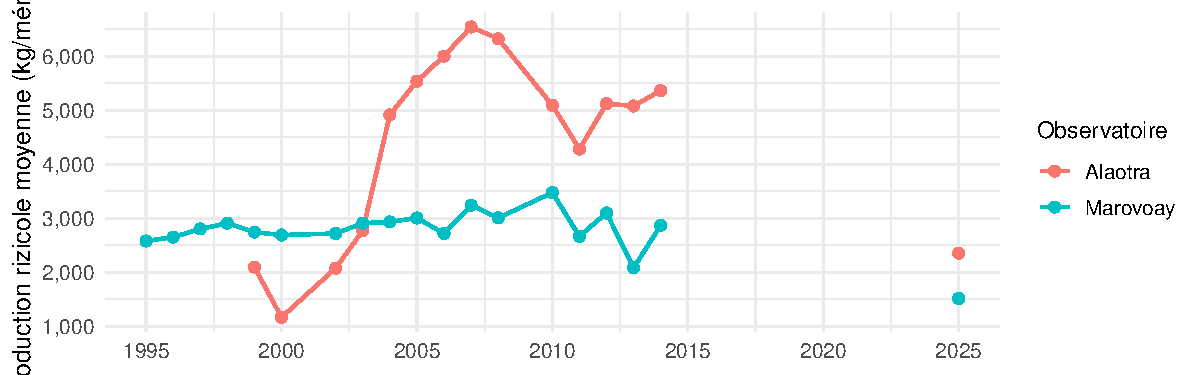
\includegraphics[keepaspectratio]{05_agriculture_files/figure-pdf/fig_agro_prod_riz-1.pdf}}

}

\caption{Évolution de la production rizicole moyenne par ménage
(kg/ménage/an)}

\end{figure}%

\begin{figure}[H]

{\centering \pandocbounded{
\includegraphics[keepaspectratio]{05_agriculture_files/figure-pdf/fig_agro_rdt_riz-1.pdf}}

}

\caption{Évolution du rendement rizicole moyen (kg/are) --- années avec
données de surface}

\end{figure}%

\begin{figure}[H]

{\centering \pandocbounded{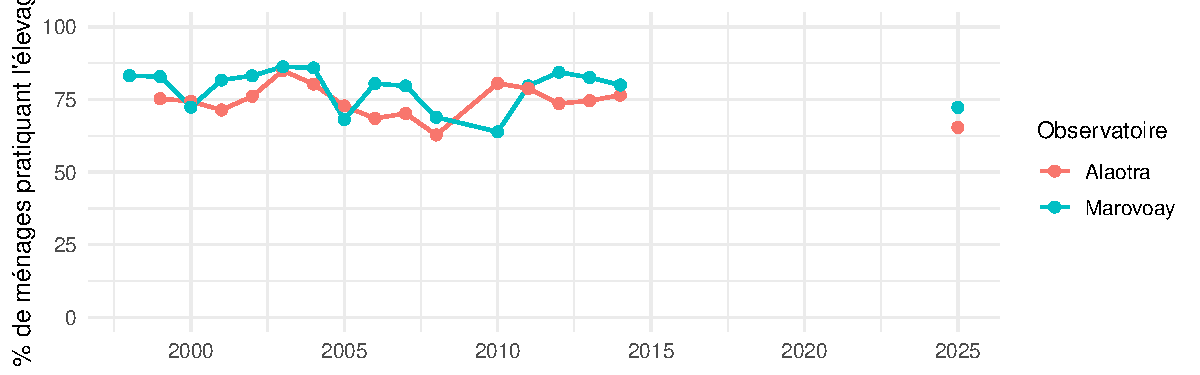
\includegraphics[keepaspectratio]{05_agriculture_files/figure-pdf/fig_agro_elevage-1.pdf}}

}

\caption{Évolution du taux de pratique de l'élevage (1998--2025)}

\end{figure}%

Les séries longues mettent en évidence des tendances structurelles :
évolution de la production rizicole par ménage, variation des rendements
en lien avec les aléas climatiques et l'intensification des pratiques,
et évolution du taux de pratique de l'élevage. La rupture de série entre
2015 et 2025 (représentée en pointillés) invite à la prudence dans
l'interprétation.

\section{Pistes d'analyse complémentaires}\label{sec-pistes-agro}

Les données collectées offrent des possibilités d'analyse
supplémentaires qui n'ont pas été développées dans ce chapitre, faute de
certitude sur leur pertinence ou par manque de recul sur la qualité des
variables concernées. On peut notamment mentionner :

\begin{itemize}
\tightlist
\item
  \textbf{Détail des ventes de riz} (\texttt{res\_dc20}) : les variables
  \texttt{vs1} à \texttt{vs3} semblent décomposent les usages du riz
  vendu (semence, consommation, paiement de main d'œuvre), mais leur
  codage est un peu complexe/à préciser.
\item
  \textbf{Forme des produits vendus} (cultures non rizicoles,
  \texttt{c37}) : la variable indique si le produit est vendu brut,
  transformé ou autre --- potentiellement utile pour un tableau croisé
  avec les types de culture.
\item
  \textbf{Coûts détaillés de la main d'œuvre par opération rizicole}
  (\texttt{res\_mor}, \texttt{mor12}) : le salaire total par opération
  (Asa tany, Mijinja, Manetsa) pourrait être présenté sous forme de
  tableau comparatif, mais les valeurs présentent une forte dispersion.
\item
  \textbf{Pratiques de nourriture de la main d'oeuvre}
  (\texttt{res\_mor}, \texttt{mor3}) : la variable indique si les
  salariés ou l'entraide sont nourris pendant le travail.
\item
  \textbf{Effectifs et variations du cheptel} (\texttt{res\_ele}) : les
  variables \texttt{ele1} (effectif début), \texttt{ele2} (naissances),
  \texttt{ele3} (achats), \texttt{ele\_i1} (ventes), \texttt{ele\_p3}
  (pertes) permettraient de reconstituer un bilan démographique du
  cheptel par espèce (difficile à exploiter à première vue).
\end{itemize}

\bookmarksetup{startatroot}

\chapter{Sécurité alimentaire}\label{suxe9curituxe9-alimentaire}

Ce chapitre traite de la sécurité alimentaire des ménages des
observatoires ruraux d'Alaotra et de Marovoay. Il aborde trois
dimensions : la période de soudure et le stress alimentaire,
l'alimentation de base hors et pendant la soudure, et les stratégies
d'adaptation adoptées par les ménages.

\begin{tcolorbox}[enhanced jigsaw, colframe=quarto-callout-warning-color-frame, colback=white, titlerule=0mm, colbacktitle=quarto-callout-warning-color!10!white, toptitle=1mm, opacitybacktitle=0.6, title=\textcolor{quarto-callout-warning-color}{\faExclamationTriangle}\hspace{0.5em}{Travail de vérification en cours}, left=2mm, leftrule=.75mm, bottomtitle=1mm, coltitle=black, arc=.35mm, rightrule=.15mm, bottomrule=.15mm, toprule=.15mm, opacityback=0, breakable]

Les résultats présentés ci-dessous sont provisoires, et sont
susceptibles de faire l'objet de corrections.

\end{tcolorbox}

\section{Disponibilité alimentaire}\label{disponibilituxe9-alimentaire}

La sécurité alimentaire des ménages ruraux est étroitement liée au
calendrier agricole et à la gestion des stocks.

\textbf{Alaotra.} 100 \% des ménages déclarent au moins un mois de
soudure.

\textbf{Marovoay.} 97.3 \% des ménages déclarent au moins un mois de
soudure.

\subsection{Période de soudure}\label{puxe9riode-de-soudure}

La période de soudure désigne les mois durant lesquels les stocks
alimentaires du ménage sont insuffisants pour couvrir ses besoins.

\textbf{Alaotra.} La soudure dure en moyenne 3.8 mois (médiane : 3).

\textbf{Marovoay.} La soudure dure en moyenne 2.2 mois (médiane : 2).

\subsubsection{Durée de la soudure par
observatoire}\label{duruxe9e-de-la-soudure-par-observatoire}

\begin{table}
\caption*{
{\fontsize{20}{25}\selectfont  Durée de la période de soudure par observatoire\fontsize{12}{15}\selectfont } \\ 
{\fontsize{14}{17}\selectfont  Nombre de mois de soudure (sal2d)\fontsize{12}{15}\selectfont }
} 
\fontsize{12.0pt}{14.0pt}\selectfont
\begin{tabular*}{\linewidth}{@{\extracolsep{\fill}}lrrrrrr}
\toprule
{\bfseries Observatory} & Nombre de ménages & {\bfseries Minimum} & Médiane & {\bfseries Moyenne} & {\bfseries Maximum} & Écart-type \\ 
\midrule\addlinespace[2.5pt]
Alaotra & 507 & 1 & 3 & 3.8 & 12 & 1.8 \\ 
Marovoay & 519 & 0 & 2 & 2.2 & 11 & 1.4 \\ 
\bottomrule
\end{tabular*}
\end{table}

\subsubsection{Durée de la soudure par hameau et
observatoire}\label{duruxe9e-de-la-soudure-par-hameau-et-observatoire}

\begin{table}
\caption*{
{\fontsize{20}{25}\selectfont  Durée moyenne de la soudure par hameau et observatoire\fontsize{12}{15}\selectfont }
} 
\fontsize{12.0pt}{14.0pt}\selectfont
\begin{tabular*}{\linewidth}{@{\extracolsep{\fill}}lr}
\toprule
Hameau & Mois de soudure (moy.) \\ 
\midrule\addlinespace[2.5pt]
\multicolumn{2}{l}{Alaotra} \\[2.5pt] 
\midrule\addlinespace[2.5pt]
Ambatoharanana & 4.1 \\ 
Ambatomanga & 4.4 \\ 
Ambodivoara & 4.3 \\ 
Ambohidrony & 4.8 \\ 
Analamiranga & 3.6 \\ 
Avaradrano & 3.1 \\ 
Feramanga Atsimo & 3.4 \\ 
Mangabe & 3.7 \\ 
{\bfseries {Ensemble}} & {\bfseries {3.8}} \\ 
\midrule\addlinespace[2.5pt]
\multicolumn{2}{l}{Marovoay} \\[2.5pt] 
\midrule\addlinespace[2.5pt]
Ampijoroa & 1.9 \\ 
Bepako & 1.9 \\ 
Madiromiongana & 2.8 \\ 
Maroala & 2.2 \\ 
{\bfseries {Ensemble}} & {\bfseries {2.2}} \\ 
\bottomrule
\end{tabular*}
\end{table}

\subsubsection{Distribution du nombre de mois de
soudure}\label{distribution-du-nombre-de-mois-de-soudure}

\pandocbounded{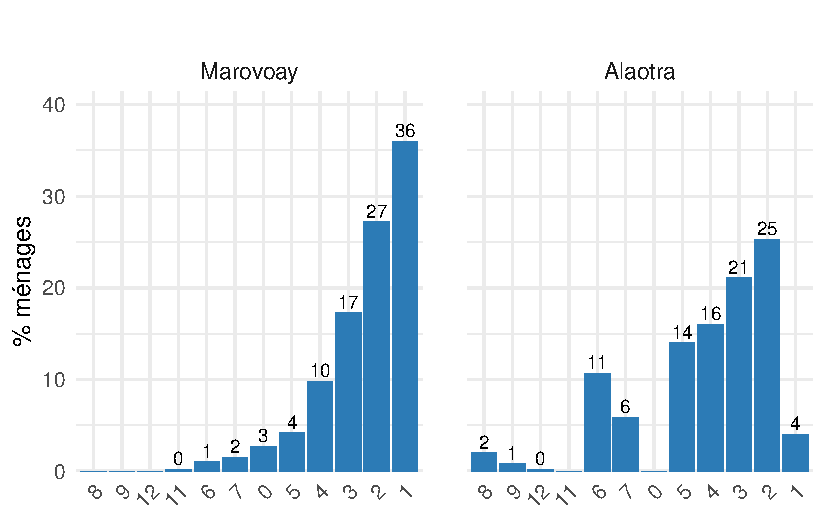
\includegraphics[keepaspectratio]{06_securite_alimentaire_files/figure-pdf/g1_soudure_distrib-1.pdf}}

\subsubsection{Calendrier de la soudure}\label{calendrier-de-la-soudure}

\begin{table}
\caption*{
{\fontsize{20}{25}\selectfont  Calendrier de la soudure par observatoire\fontsize{12}{15}\selectfont } \\ 
{\fontsize{14}{17}\selectfont  \% de ménages en période de soudure chaque mois\fontsize{12}{15}\selectfont }
} 
\fontsize{12.0pt}{14.0pt}\selectfont
\begin{tabular*}{\linewidth}{@{\extracolsep{\fill}}crr}
\toprule
{\bfseries Mois} & {\bfseries Alaotra} & {\bfseries Marovoay} \\ 
\midrule\addlinespace[2.5pt]
Octobre & 37.5 & 24.9 \\ 
Novembre & 32.7 & 23.1 \\ 
Décembre & 31.8 & 22.0 \\ 
Janvier & 40.0 & 39.3 \\ 
Février & 60.7 & 65.3 \\ 
Mars & 86.8 & 52.4 \\ 
Avril & 49.9 & 20.6 \\ 
Mai & 3.2 & 6.2 \\ 
Juin & 0.2 & 4.8 \\ 
Juillet & 2.8 & 5.2 \\ 
Août & 12.8 & 7.7 \\ 
Septembre & 27.0 & 11.9 \\ 
\bottomrule
\end{tabular*}
\end{table}

\pandocbounded{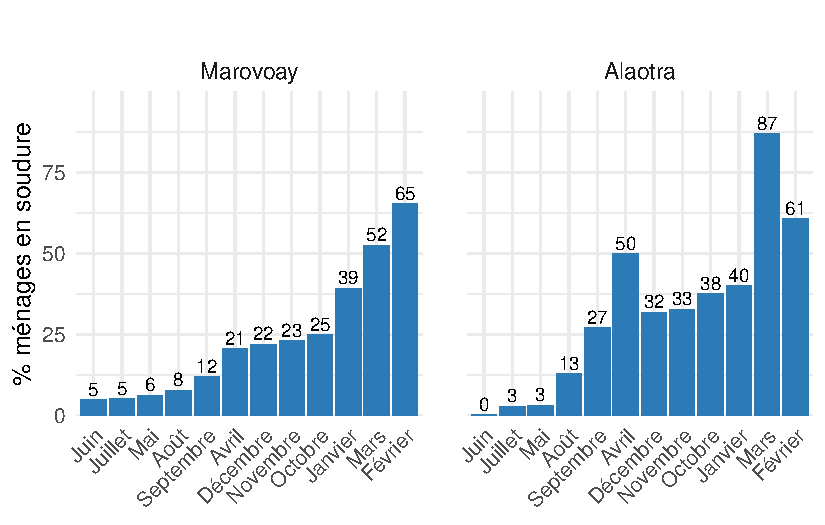
\includegraphics[keepaspectratio]{06_securite_alimentaire_files/figure-pdf/g2_calendrier_soudure-1.pdf}}

\subsection{Stress alimentaire}\label{stress-alimentaire}

Le stress alimentaire reflète les mois durant lesquels le ménage éprouve
des difficultés à se nourrir correctement, que ce soit en quantité ou en
qualité. Sa durée est généralement supérieure à celle de la soudure
stricto sensu.

\textbf{Alaotra.} La durée moyenne du stress alimentaire atteint 2.5
mois.

\textbf{Marovoay.} La durée moyenne du stress alimentaire atteint 3.3
mois.

\subsubsection{Durée du stress alimentaire par
observatoire}\label{duruxe9e-du-stress-alimentaire-par-observatoire}

\begin{table}
\caption*{
{\fontsize{20}{25}\selectfont  Durée du stress alimentaire par observatoire\fontsize{12}{15}\selectfont } \\ 
{\fontsize{14}{17}\selectfont  Nombre de mois de stress alimentaire (sal15a)\fontsize{12}{15}\selectfont }
} 
\fontsize{12.0pt}{14.0pt}\selectfont
\begin{tabular*}{\linewidth}{@{\extracolsep{\fill}}lrrrrrr}
\toprule
{\bfseries Observatory} & Nombre de ménages & {\bfseries Minimum} & Médiane & {\bfseries Moyenne} & {\bfseries Maximum} & Écart-type \\ 
\midrule\addlinespace[2.5pt]
Alaotra & 507 & 0 & 2 & 2.5 & 12 & 1.6 \\ 
Marovoay & 519 & 0 & 3 & 3.3 & 12 & 2.0 \\ 
\bottomrule
\end{tabular*}
\end{table}

\subsubsection{Calendrier du stress
alimentaire}\label{calendrier-du-stress-alimentaire}

\begin{table}
\caption*{
{\fontsize{20}{25}\selectfont  Calendrier du stress alimentaire par observatoire\fontsize{12}{15}\selectfont } \\ 
{\fontsize{14}{17}\selectfont  \% de ménages en stress alimentaire chaque mois\fontsize{12}{15}\selectfont }
} 
\fontsize{12.0pt}{14.0pt}\selectfont
\begin{tabular*}{\linewidth}{@{\extracolsep{\fill}}crr}
\toprule
{\bfseries Mois} & {\bfseries Alaotra} & {\bfseries Marovoay} \\ 
\midrule\addlinespace[2.5pt]
Octobre & 23.5 & 35.1 \\ 
Novembre & 18.1 & 31.4 \\ 
Décembre & 13.2 & 30.6 \\ 
Janvier & 21.1 & 47.4 \\ 
Février & 38.5 & 67.6 \\ 
Mars & 74.8 & 59.2 \\ 
Avril & 35.3 & 27.2 \\ 
Mai & 2.6 & 11.2 \\ 
Juin & 0.4 & 9.6 \\ 
Juillet & 2.0 & 10.4 \\ 
Août & 8.5 & 13.3 \\ 
Septembre & 17.0 & 17.3 \\ 
\bottomrule
\end{tabular*}
\end{table}

\subsubsection{Comparaison soudure et stress
alimentaire}\label{comparaison-soudure-et-stress-alimentaire}

\pandocbounded{
\includegraphics[keepaspectratio]{06_securite_alimentaire_files/figure-pdf/g3_soudure_vs_stress-1.pdf}}

\subsection{Alimentation de base}\label{alimentation-de-base}

Cette section compare les aliments de base consommés aux trois repas,
hors et pendant la période de soudure. Le riz constitue la base
alimentaire dans les deux observatoires, mais sa place relative varie
selon la saison et le site. Les substitutions opérées pendant la soudure
(manioc, patate douce, maïs) témoignent des stratégies d'adaptation
alimentaire des ménages.

\subsubsection{Alimentation hors
soudure}\label{alimentation-hors-soudure}

\begin{table}
\caption*{
{\fontsize{20}{25}\selectfont  Alimentation de base hors soudure par observatoire\fontsize{12}{15}\selectfont } \\ 
{\fontsize{14}{17}\selectfont  Aliments représentant au moins 2\% des réponses\fontsize{12}{15}\selectfont }
} 
\fontsize{12.0pt}{14.0pt}\selectfont
\begin{tabular*}{\linewidth}{@{\extracolsep{\fill}}llr}
\toprule
{\bfseries Repas} & {\bfseries Aliment} & \% \\ 
\midrule\addlinespace[2.5pt]
\multicolumn{3}{l}{Alaotra} \\[2.5pt] 
\midrule\addlinespace[2.5pt]
Déjeuner & Riz & 93.5 \\ 
Déjeuner & Manioc & 4.0 \\ 
Dîner & Riz & 99.6 \\ 
Petit-déjeuner & Riz & 97.8 \\ 
\midrule\addlinespace[2.5pt]
\multicolumn{3}{l}{Marovoay} \\[2.5pt] 
\midrule\addlinespace[2.5pt]
Déjeuner & Riz & 95.2 \\ 
Déjeuner & Maïs & 2.5 \\ 
Dîner & Riz & 99.6 \\ 
Petit-déjeuner & Riz & 89.9 \\ 
Petit-déjeuner & Rien & 2.7 \\ 
Petit-déjeuner & Boisson chaude & 2.3 \\ 
\bottomrule
\end{tabular*}
\end{table}

\subsubsection{Alimentation pendant la
soudure}\label{alimentation-pendant-la-soudure}

\begin{table}
\caption*{
{\fontsize{20}{25}\selectfont  Alimentation de base pendant la soudure par observatoire\fontsize{12}{15}\selectfont } \\ 
{\fontsize{14}{17}\selectfont  Aliments représentant au moins 2\% des réponses\fontsize{12}{15}\selectfont }
} 
\fontsize{12.0pt}{14.0pt}\selectfont
\begin{tabular*}{\linewidth}{@{\extracolsep{\fill}}llr}
\toprule
{\bfseries Repas} & {\bfseries Aliment} & \% \\ 
\midrule\addlinespace[2.5pt]
\multicolumn{3}{l}{Alaotra} \\[2.5pt] 
\midrule\addlinespace[2.5pt]
Déjeuner & Riz & 52.6 \\ 
Déjeuner & Manioc & 27.4 \\ 
Déjeuner & Maïs & 16.7 \\ 
Dîner & Riz & 98.0 \\ 
Petit-déjeuner & Riz & 92.0 \\ 
Petit-déjeuner & Rien & 3.6 \\ 
\midrule\addlinespace[2.5pt]
\multicolumn{3}{l}{Marovoay} \\[2.5pt] 
\midrule\addlinespace[2.5pt]
Déjeuner & Riz & 60.8 \\ 
Déjeuner & Maïs & 20.7 \\ 
Déjeuner & Manioc & 11.5 \\ 
Déjeuner & Patate douce & 4.6 \\ 
Dîner & Riz & 92.5 \\ 
Dîner & Manioc & 2.6 \\ 
Dîner & Maïs & 2.4 \\ 
Petit-déjeuner & Riz & 55.7 \\ 
Petit-déjeuner & Rien & 25.3 \\ 
Petit-déjeuner & Manioc & 6.1 \\ 
Petit-déjeuner & Boisson chaude & 3.6 \\ 
Petit-déjeuner & Maïs & 3.4 \\ 
Petit-déjeuner & Patate douce & 2.8 \\ 
\bottomrule
\end{tabular*}
\end{table}

\subsubsection{Comparaison de l'alimentation au déjeuner : hors vs
pendant
soudure}\label{comparaison-de-lalimentation-au-duxe9jeuner-hors-vs-pendant-soudure}

\pandocbounded{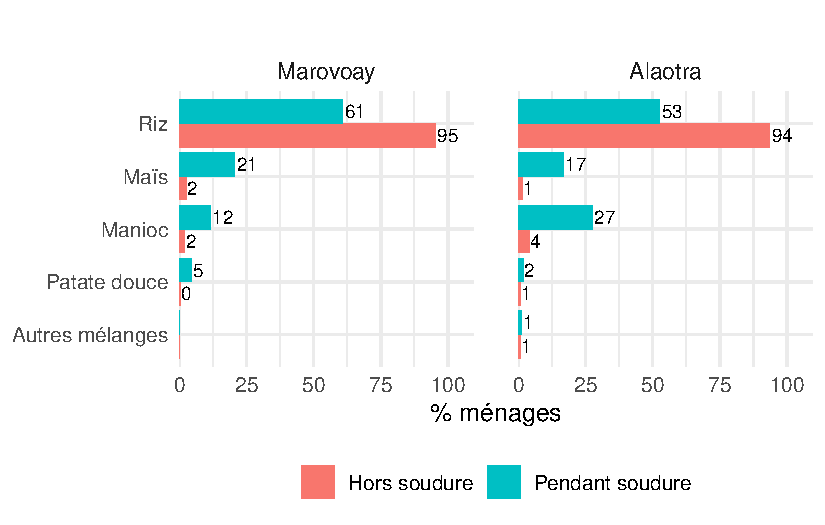
\includegraphics[keepaspectratio]{06_securite_alimentaire_files/figure-pdf/g4_comparaison_dejeuner-1.pdf}}

\subsubsection{Changement d'aliment de base au déjeuner entre hors et
pendant
soudure}\label{changement-daliment-de-base-au-duxe9jeuner-entre-hors-et-pendant-soudure}

\begin{table}
\caption*{
{\fontsize{20}{25}\selectfont  Changement d'aliment de base au déjeuner\fontsize{12}{15}\selectfont } \\ 
{\fontsize{14}{17}\selectfont  Transitions hors soudure \textrightarrow pendant soudure (\ensuremath{\geq} 1\%)\fontsize{12}{15}\selectfont }
} 
\fontsize{12.0pt}{14.0pt}\selectfont
\begin{tabular*}{\linewidth}{@{\extracolsep{\fill}}llrr}
\toprule
Hors soudure & Pendant soudure & Effectif & \% \\ 
\midrule\addlinespace[2.5pt]
\multicolumn{4}{l}{Alaotra} \\[2.5pt] 
\midrule\addlinespace[2.5pt]
Riz & Riz & 259 & 52.2 \\ 
Riz & Manioc & 116 & 23.4 \\ 
Riz & Maïs & 76 & 15.3 \\ 
Manioc & Manioc & 18 & 3.6 \\ 
Riz & Patate douce & 6 & 1.2 \\ 
Riz & Autres mélanges & 5 & 1.0 \\ 
\midrule\addlinespace[2.5pt]
\multicolumn{4}{l}{Marovoay} \\[2.5pt] 
\midrule\addlinespace[2.5pt]
Riz & Riz & 305 & 60.6 \\ 
Riz & Maïs & 91 & 18.1 \\ 
Riz & Manioc & 49 & 9.7 \\ 
Riz & Patate douce & 21 & 4.2 \\ 
Maïs & Maïs & 11 & 2.2 \\ 
Manioc & Manioc & 8 & 1.6 \\ 
Riz & Rien & 5 & 1.0 \\ 
\bottomrule
\end{tabular*}
\end{table}

\section{Stratégies de sécurité
alimentaire}\label{stratuxe9gies-de-suxe9curituxe9-alimentaire}

Face à l'insécurité alimentaire, les ménages déploient un éventail de
stratégies d'adaptation dont la sévérité varie : réduction des portions,
substitution d'aliments, endettement, cueillette sauvage, voire
décapitalisation. Chaque stratégie est évaluée sur une échelle de
fréquence : 0 = Jamais, 1 = Rarement, 2 = Quelquefois, 3 = Souvent.

\subsection{Fréquence des stratégies
d'adaptation}\label{fruxe9quence-des-stratuxe9gies-dadaptation}

\begin{table}
\caption*{
{\fontsize{20}{25}\selectfont  Stratégies d'adaptation les plus fréquentes\fontsize{12}{15}\selectfont } \\ 
{\fontsize{14}{17}\selectfont  \% de ménages ayant recours \guillemotleft Quelquefois \guillemotright ou \guillemotleft Souvent \guillemotright\fontsize{12}{15}\selectfont }
} 
\fontsize{12.0pt}{14.0pt}\selectfont
\begin{tabular*}{\linewidth}{@{\extracolsep{\fill}}lrr}
\toprule
Stratégie & Alaotra (\%) & Marovoay (\%) \\ 
\midrule\addlinespace[2.5pt]
{{Réduire la ration à chaque repas}} & {{58.2}} & {{80.5}} \\ 
Réduire/renoncer aux ingrédients chers & 51.7 & 60.2 \\ 
{{Remplacer l'aliment de base}} & {{41.1}} & {{43.8}} \\ 
Réduire le nombre de repas & 26.0 & 43.8 \\ 
{{Cueillette d'aliments sauvages}} & {{21.5}} & {{15.1}} \\ 
Emprunter des aliments & 21.4 & 14.7 \\ 
{{S'endetter pour acheter des aliments}} & {{13.8}} & {{17.7}} \\ 
Réduire les dépenses non essentielles & 7.7 & 16.2 \\ 
{{Envoyer un membre chez un autre ménage}} & {{9.7}} & {{10.8}} \\ 
Envoyer un membre travailler ailleurs & 4.4 & 5.2 \\ 
{{Faire une nouvelle activité}} & {{6.3}} & {{2.2}} \\ 
Autre stratégie & 2.7 & 3.1 \\ 
{{Vendre d'autres biens du ménage}} & {{4.4}} & {{1.4}} \\ 
Vendre des moyens de production & 3.9 & 0.2 \\ 
\bottomrule
\end{tabular*}
\end{table}

\pandocbounded{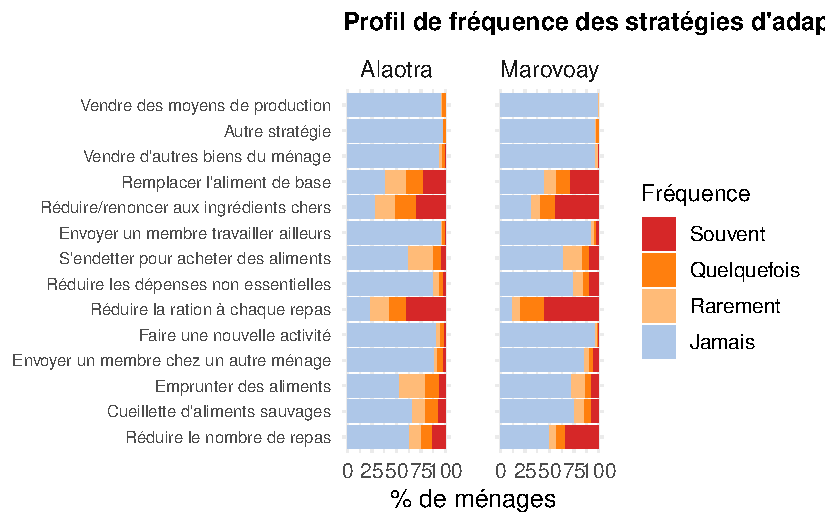
\includegraphics[keepaspectratio]{06_securite_alimentaire_files/figure-pdf/g5_strategies_likert-1.pdf}}

\subsection{Sources d'endettement et d'emprunt
alimentaire}\label{sources-dendettement-et-demprunt-alimentaire}

\begin{table}
\caption*{
{\fontsize{20}{25}\selectfont  Sources d'endettement pour achat alimentaire\fontsize{12}{15}\selectfont } \\ 
{\fontsize{14}{17}\selectfont  Parmi les ménages qui s'endettent (ssa01 > 0)\fontsize{12}{15}\selectfont }
} 
\fontsize{12.0pt}{14.0pt}\selectfont
\begin{tabular*}{\linewidth}{@{\extracolsep{\fill}}lrrrr}
\toprule
 & \multicolumn{2}{c}{{\bfseries Alaotra}} & \multicolumn{2}{c}{{\bfseries Marovoay}} \\ 
\cmidrule(lr){2-3} \cmidrule(lr){4-5}
{\bfseries Source} & N & \% & N & \% \\ 
\midrule\addlinespace[2.5pt]
Autres & 3 & 1.6 & 20 & 10.8 \\ 
Commerçants & 7 & 3.6 & 4 & 2.1 \\ 
Famille & 127 & 64.1 & 84 & 44.0 \\ 
Usuriers & 13 & 6.6 & 34 & 17.8 \\ 
Voisins & 80 & 40.6 & 63 & 33.0 \\ 
\bottomrule
\end{tabular*}
\end{table}

\begin{table}
\caption*{
{\fontsize{20}{25}\selectfont  Sources d'emprunt d'aliments de base\fontsize{12}{15}\selectfont } \\ 
{\fontsize{14}{17}\selectfont  Parmi les ménages qui empruntent des aliments (ssa02 > 0)\fontsize{12}{15}\selectfont }
} 
\fontsize{12.0pt}{14.0pt}\selectfont
\begin{tabular*}{\linewidth}{@{\extracolsep{\fill}}lrrrr}
\toprule
 & \multicolumn{2}{c}{{\bfseries Alaotra}} & \multicolumn{2}{c}{{\bfseries Marovoay}} \\ 
\cmidrule(lr){2-3} \cmidrule(lr){4-5}
{\bfseries Source} & N & \% & N & \% \\ 
\midrule\addlinespace[2.5pt]
Autres & 4 & 1.7 & 2 & 1.4 \\ 
Commerçants & 66 & 28.0 & 10 & 6.9 \\ 
Famille & 107 & 45.5 & 85 & 58.6 \\ 
Usuriers & 4 & 1.7 & 8 & 5.6 \\ 
Voisins & 82 & 35.0 & 39 & 27.1 \\ 
\bottomrule
\end{tabular*}
\end{table}

\pandocbounded{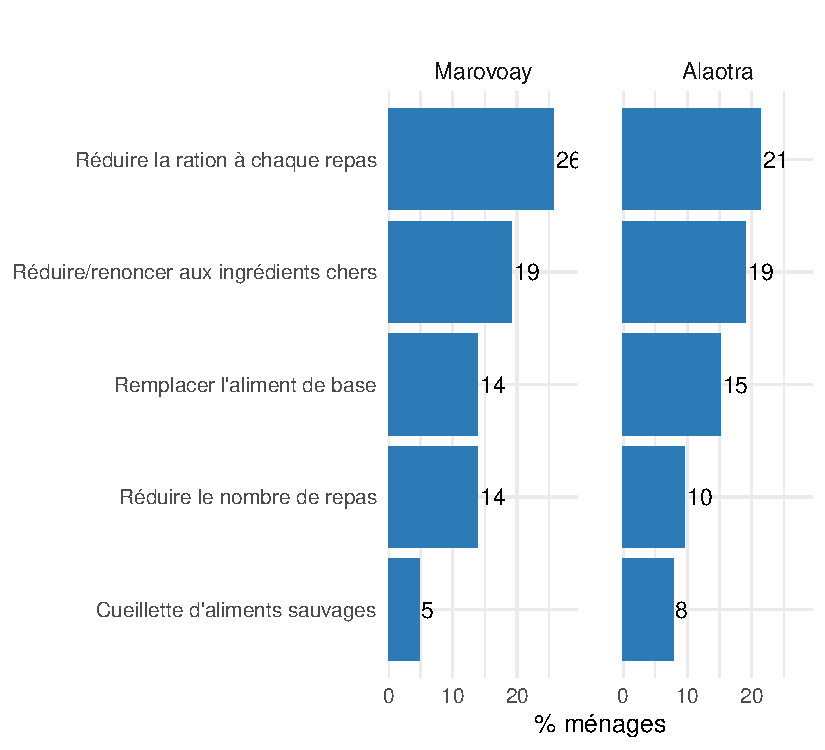
\includegraphics[keepaspectratio]{06_securite_alimentaire_files/figure-pdf/g6_top_strategies-1.pdf}}

\section{Indice synthétique de stratégies d'adaptation (CSI
simplifié)}\label{indice-synthuxe9tique-de-stratuxe9gies-dadaptation-csi-simplifiuxe9}

Un score simplifié est calculé en sommant les fréquences de toutes les
stratégies (0 à 3) pour chaque ménage. Plus le score est élevé, plus le
ménage recourt intensément à des stratégies d'adaptation.

\begin{table}
\caption*{
{\fontsize{20}{25}\selectfont  Score CSI simplifié par hameau et observatoire\fontsize{12}{15}\selectfont } \\ 
{\fontsize{14}{17}\selectfont  Somme des fréquences des stratégies (0\textendash3 par stratégie)\fontsize{12}{15}\selectfont }
} 
\fontsize{12.0pt}{14.0pt}\selectfont
\begin{tabular*}{\linewidth}{@{\extracolsep{\fill}}lrr}
\toprule
Hameau & Nb ménages & Score CSI moyen \\ 
\midrule\addlinespace[2.5pt]
\multicolumn{3}{l}{Alaotra} \\[2.5pt] 
\midrule\addlinespace[2.5pt]
Ambatoharanana & 31 & 7.2 \\ 
Ambatomanga & 68 & 8.6 \\ 
Ambodivoara & 58 & 8.3 \\ 
Ambohidrony & 52 & 9.0 \\ 
Analamiranga & 46 & 8.5 \\ 
Avaradrano & 90 & 6.8 \\ 
Feramanga Atsimo & 89 & 10.1 \\ 
Mangabe & 73 & 8.5 \\ 
{\bfseries {Ensemble}} & {\bfseries {507}} & {\bfseries {8.4}} \\ 
\midrule\addlinespace[2.5pt]
\multicolumn{3}{l}{Marovoay} \\[2.5pt] 
\midrule\addlinespace[2.5pt]
Ampijoroa & 143 & 9.6 \\ 
Bepako & 123 & 9.1 \\ 
Madiromiongana & 137 & 9.3 \\ 
Maroala & 116 & 10.0 \\ 
{\bfseries {Ensemble}} & {\bfseries {519}} & {\bfseries {9.5}} \\ 
\bottomrule
\end{tabular*}
\end{table}

\pandocbounded{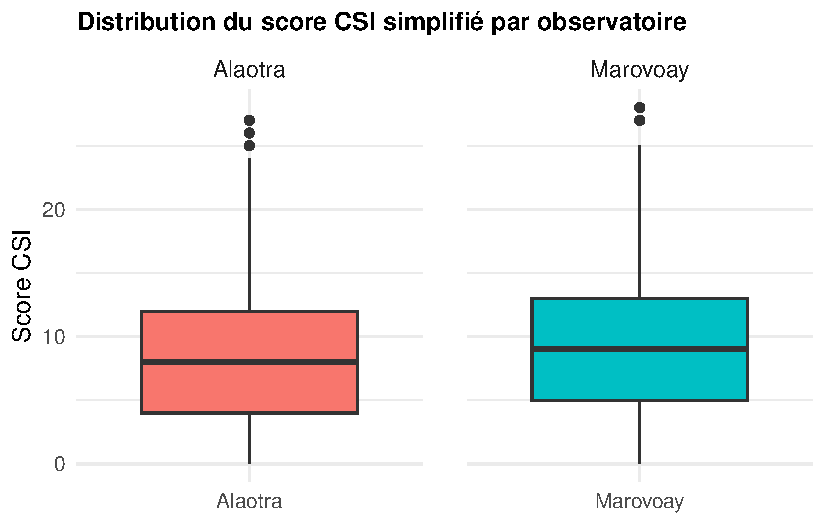
\includegraphics[keepaspectratio]{06_securite_alimentaire_files/figure-pdf/g7_csi_boxplot-1.pdf}}

\section{Évolution de la sécurité alimentaire
(1995--2025)}\label{sec-sa-multiyear}

La durée de la période de soudure (\texttt{sal2d}, en mois) est
disponible pour un nombre significatif de campagnes. On retrace ici son
évolution pour les deux observatoires.

\begin{figure}[H]

{\centering \pandocbounded{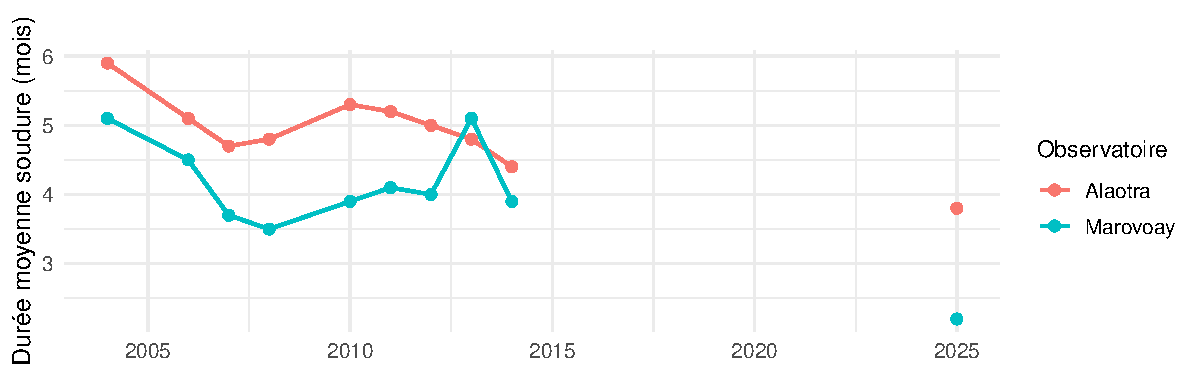
\includegraphics[keepaspectratio]{06_securite_alimentaire_files/figure-pdf/fig_sa_soudure_duration-1.pdf}}

}

\caption{Évolution de la durée moyenne de soudure (mois/ménage)}

\end{figure}%

\begin{figure}[H]

{\centering \pandocbounded{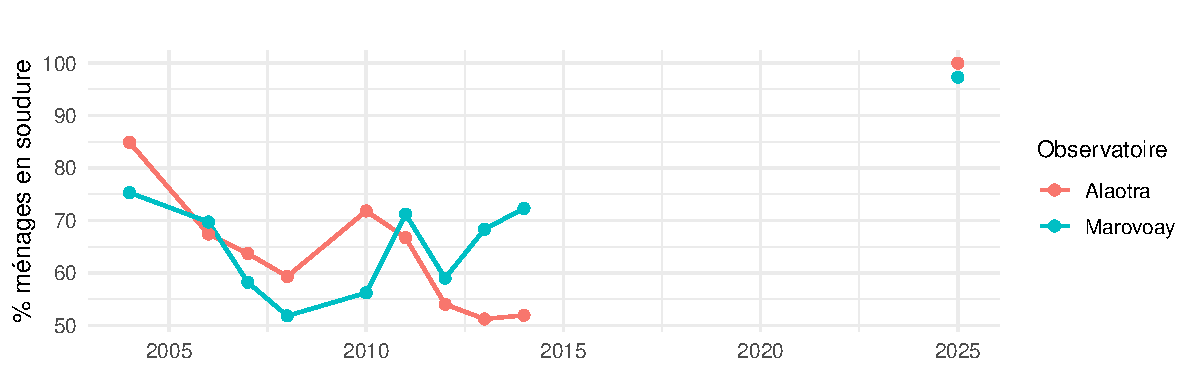
\includegraphics[keepaspectratio]{06_securite_alimentaire_files/figure-pdf/fig_sa_pct_soudure-1.pdf}}

}

\caption{Évolution du pourcentage de ménages en soudure}

\end{figure}%

\bookmarksetup{startatroot}

\chapter{Rapport des ménages ruraux avec
l'environnement}\label{rapport-des-muxe9nages-ruraux-avec-lenvironnement}

Les deux observatoires sont situés à proximité d'aires protégées
majeures : Pour Alaotra la Nouvelle Aire Protégée du lac Alaotra et le
Corridor Ankeniheny Zahamena et pour Marovoay le Parc National
d'Ankarafantsika. Ce chapitre analyse les représentations, les usages,
les pratiques (notamment le feu) et les opinions des ménages concernant
la protection de l'environnement.

\begin{tcolorbox}[enhanced jigsaw, colframe=quarto-callout-warning-color-frame, colback=white, titlerule=0mm, colbacktitle=quarto-callout-warning-color!10!white, toptitle=1mm, opacitybacktitle=0.6, title=\textcolor{quarto-callout-warning-color}{\faExclamationTriangle}\hspace{0.5em}{Travail de vérification en cours}, left=2mm, leftrule=.75mm, bottomtitle=1mm, coltitle=black, arc=.35mm, rightrule=.15mm, bottomrule=.15mm, toprule=.15mm, opacityback=0, breakable]

Les résultats présentés ci-dessous sont provisoires, et sont
susceptibles de faire l'objet de corrections.

\end{tcolorbox}

\section{Représentation de la zone protégée par les
ménages}\label{sec-representation}

\subsection{Caractérisation de la zone : disponibilité des
ressources}\label{caractuxe9risation-de-la-zone-disponibilituxe9-des-ressources}

Les ménages ont été interrogés sur la disponibilité de dix catégories de
ressources naturelles dans la zone protégée à proximité de leur village.
La Figure~\ref{fig-ressources-dispo} résume les réponses, distinguant
les ressources jugées abondantes, en quantité normale ou rares.

\begin{figure}

\centering{

\pandocbounded{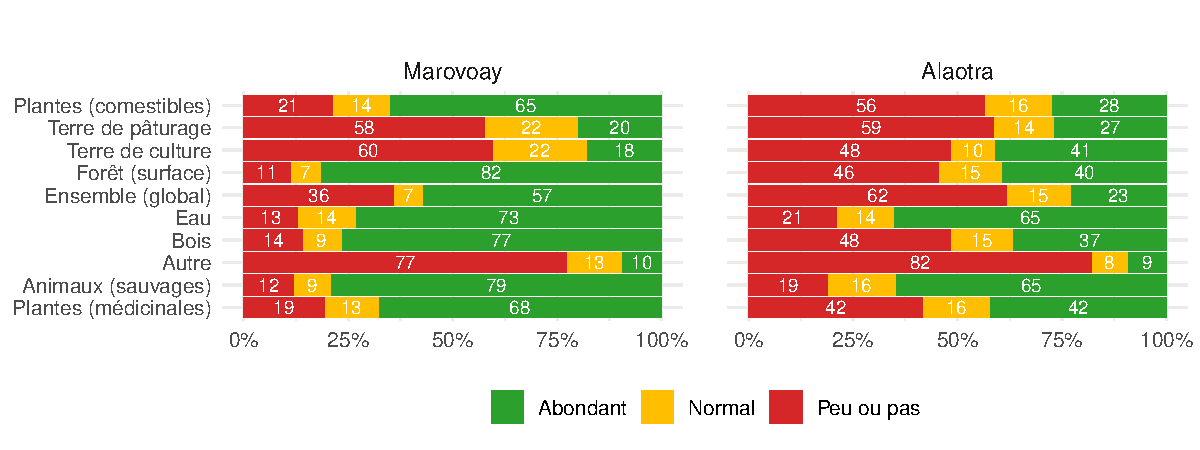
\includegraphics[keepaspectratio]{07_rapport_environnement_files/figure-pdf/fig-ressources-dispo-1.pdf}}

}

\caption{\label{fig-ressources-dispo}Disponibilité perçue des ressources
naturelles dans la zone protégée, par observatoire}

\end{figure}%

\subsection{Évolution perçue des
ressources}\label{uxe9volution-peruxe7ue-des-ressources}

Les ménages estiment l'évolution de ces ressources sur les trois et cinq
dernières années. La Figure~\ref{fig-evolution-ressources} présente la
tendance à 3 ans.

\begin{figure}

\centering{

\pandocbounded{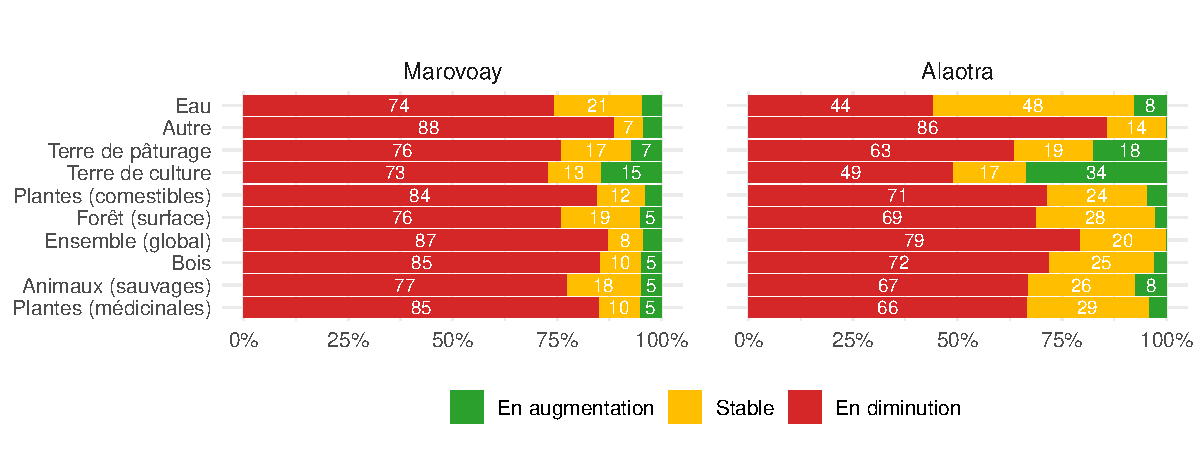
\includegraphics[keepaspectratio]{07_rapport_environnement_files/figure-pdf/fig-evolution-ressources-1.pdf}}

}

\caption{\label{fig-evolution-ressources}Évolution perçue des ressources
naturelles au cours des 3 dernières années}

\end{figure}%

\subsection{Appartenance perçue de la
zone}\label{appartenance-peruxe7ue-de-la-zone}

La question RM3 demande à qui appartient la zone protégée (réponses
multiples). La Figure~\ref{fig-appartenance} montre les réponses par
observatoire.

\begin{figure}

\centering{

\pandocbounded{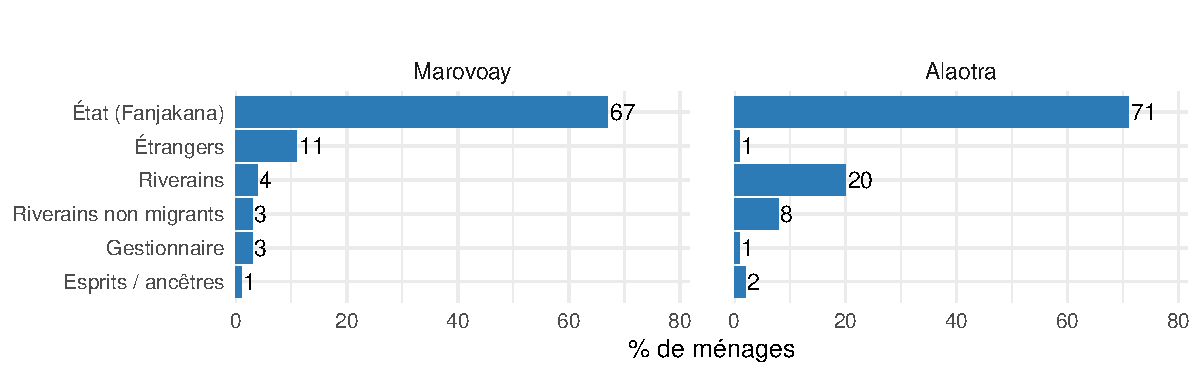
\includegraphics[keepaspectratio]{07_rapport_environnement_files/figure-pdf/fig-appartenance-1.pdf}}

}

\caption{\label{fig-appartenance}À qui appartient la zone protégée ? (\%
de Oui, réponses multiples)}

\end{figure}%

\subsection{Menaces perçues et
responsables}\label{menaces-peruxe7ues-et-responsables}

Les ménages ont été interrogés sur les menaces qu'ils perçoivent
vis-à-vis de l'environnement local et sur les responsables qu'ils
identifient. Ces perceptions reflètent la conscience environnementale
des populations et orientent les stratégies de sensibilisation.

\begin{table}

\caption{\label{tbl-menaces}Menaces perçues sur l'environnement et
responsables identifiés (\% de Oui)}

\centering{

\fontsize{12.0pt}{14.0pt}\selectfont
\begin{tabular*}{\linewidth}{@{\extracolsep{\fill}}lrr}
\toprule
 & {\bfseries {Alaotra}} & {\bfseries {Marovoay}} \\ 
\midrule\addlinespace[2.5pt]
\multicolumn{3}{l}{{\bfseries {Perception globale}}} \\[2.5pt] 
\midrule\addlinespace[2.5pt]
Considèrent que l'environnement est menacé & 82 % & 79 % \\ 
\midrule\addlinespace[2.5pt]
\multicolumn{3}{l}{{\bfseries {Principales menaces (parmi ceux qui déclarent menacé)}}} \\[2.5pt] 
\midrule\addlinespace[2.5pt]
Feux & 84 % & 95 % \\ 
Défrichage & 56 % & 52 % \\ 
Prélèvement (faune) & 40 % & 20 % \\ 
Prélèvement (flore) & 40 % & 21 % \\ 
Prospection minière & 29 % & 6 % \\ 
Nomadisme (passage non-résidents) & 16 % & 16 % \\ 
Zébu / pâturage & 20 % & 10 % \\ 
Tourisme & 2 % & 3 % \\ 
\midrule\addlinespace[2.5pt]
\multicolumn{3}{l}{{\bfseries {Principaux responsables}}} \\[2.5pt] 
\midrule\addlinespace[2.5pt]
L'ensemble des riverains & 87 % & 70 % \\ 
Les riverains migrants & 47 % & 37 % \\ 
L'État (Fanjakana) & 10 % & 8 % \\ 
Les braconniers & 30 % & 10 % \\ 
Le gestionnaire & 9 % & 3 % \\ 
Les nomades ou semi-nomades & 22 % & 17 % \\ 
Les ONG ou entreprises & 3 % & 4 % \\ 
Les chercheurs & 0 % & 2 % \\ 
Les touristes & 1 % & 2 % \\ 
\bottomrule
\end{tabular*}
\begin{minipage}{\linewidth}
\textbf{Source : Enquête auprès des OR 2025}\\
\end{minipage}

}

\end{table}%
\end{document}
